\documentclass[a4paper,10pt]{article}
%\pdfoutput=1 % if your are submitting a pdflatex (i.e. if you have
             % images in pdf, png or jpg format)
\usepackage{jheppub} % for details on the use of the package, please
                     % see the JHEP-author-manual
\usepackage[T1]{fontenc} % if needed

\usepackage{slashed}
%\usepackage{subfigure}
\usepackage{xspace}
\usepackage{booktabs}
%% %simple case: 2 authors, same institution
%% \author{A. Uthor}
%% \author{and A. Nother Author}
%% \affiliation{Institution,\\Address, Country}


\title{\boldmath Extending the pMSSM Coverage with 3-jets+$E_T ^{miss}$ Simplified Models Results}

\author[a]{Federico Ambrogi}
\affiliation[a]{University of Vienna, Faculty of Physics, Bolzmanngasse 5, A-1090 Wien, Austria}
% e-mail addresses: one for each author, in the same order as the authors\emailAdd{federico.ambrogi@oeaw.ac.at}
\emailAdd{federico.ambrogi88@gmail.com}


%%% Various Tools
\newcommand{\amc}{{\sc MadGraph5\textunderscore}a{\sc MC@NLO}}
\newcommand{\pyE}{{\sc Pythia\,8}\xspace}
\newcommand{\pys}{{\sc Pythia\,6}\xspace}
\newcommand{\pythiaS}{{\sc Pythia\,6}\xspace}
\newcommand{\pythiaSF}{{\sc Pythia\,6.4}\xspace}
\newcommand{\pythiaSFTS}{{\sc Pythia\,6.4.27}\xspace}
\newcommand{\nllfast}{{\sc NLLfast}\xspace}
\newcommand{\delphes}{{\sc Delphes\,3}}
\newcommand{\MA}{{\sc MadAnalysis\,5}}
\newcommand{\SMO}{{\sc SModelS}}

\newcommand{\MET}{{ $E_T ^{miss}$}}
%%% Sparticles
\newcommand{\MSQ}{$ m _{ \tilde q } $\xspace} 
\newcommand{\MGLU}{$ m _{ \tilde g } $\xspace} 


\newcommand{\FASTLIM}{\texttt{FasLim}} 


\newcommand{\TGQ}{ \textit{T3GQ}} 
\newcommand{\Ttwo}{ \textit{T2}} 
\newcommand{\Tfive}{ \textit{T5}} 

\newcommand{\ONE}{\onecolumn}

\newcommand{\TWO}{\twocolumn}



\begin{document} 
\sffamily
\maketitle
\begin{abstract}
The 19-parameters realisation of the phenomenological minimal supersymmeric standard model (pMSSM) studied by the ATLAS collaboration in \href{https://arxiv.org/abs/1508.06608}{arXiv:1508.06608} can also be efficiently constrained by means of simplified models results with \SMO, as recently shown in \href{https://arxiv.org/abs/1707.09036}{arXiv:1707.09036}. By increasing the number of results published by  the ATLAS and CMS with efficiency maps results produced with recasting tools, it is possible to improve the coverage of this model and increase significantly the number of excluded points. In this work we show concretely how this can be achieved with the inclusion of the EMs results for a simplified model signature as simple as 3jets + \MET~.
\end{abstract}

\flushbottom



\sffamily
%
\TWO
%
\section{Introduction}
Simplified models spectra (SMS) have become the standard method for the LHC collaborations to interpret the results of their searches for Beyond the Standard Model (BSM) particles, as in the case of Supersymmetry (SUSY). The most notable benefit coming from the adoption of SMS is the efficient reduction of the large parameter spaces of full theories. With SMS, the impact of the LHC searches can be understood by introducing only a handful of new parameters, such as the masses of the of the SUSY particles, their production cross section and their decay modes. \\

Typically only a few SUSY particles are considered in each SMS, and all the others are considered decoupled, menaing that they are too heavy to be produced at the LHC, and to appear as intermediate states in the decay chans. Once these parameters are fixed, it is straightforward to estimate the exclusion provided by the LHC searches in terms of SMS. As a drawback, however, one has to carefully use such results to constrain general models, where complicated decay patterns are involved due to the presence of several undecoupled particles. Dedicated tools such as \FASTLIM and \SMO were developed for this scope. They can decompose the signal of e.g. SUSY models into its SMS, and check the constraints provided by the LHC searches, contained in a dedicated database of results. In particular, \SMO was used in \cite{Ambrogi:2017lov} to study the coverage of the phenomenological Minimal Supersymmetric Standard Models (pMSSM) by means of simplified model results. Specifically, the set of pMSSM points considered were made public by the ATLAS collaboration on the \texttt{HepData} website\cite{ATLASpMSSMhepdata}, and the ATLAS experiment's sensitivity of Run 1 searches for SUSY and other more exotic signatures was extensively discussed in \cite{2015baa}. In particular it was analised the fraction of pMSSM points that the ATLAS searches culd excluded accoridng to the nature of the LSP, i.e. Bino, Higgsino and Wino-like LSP. 
The total coverage obtained by the previous \SMO~study amounted to roughly 55$\%$-63$\%$ for the Bino and Higgsino-like LSP case, respectively. The Wino-like LSP dataset was neglected since most of the model pointed included long-lived charged particles, a signature which could not be handled by the version of the \SMO~software used. The work also showed that by means of efficiency maps (EM) results, particularly produced by phenomenologists outside the experimental collaborations, it was possible to increase the number of excluded point.
\\

The comparison between the \SMO~approach and the re-interpretation performed by the ATLAS collaboration, based on a full recast approach, showed that the main limitation of the simplified model approach is the lack of results for simple signatures, such as the $3jets$ +\MET~. One of the \SMO~tool main features is indeed the ability of extracting the most relevant signatures in terms of $\sigma \times BR$ (production cross section  times branching ratio) that are not currently constrained by simplified models results, called \textit{missing topologies}. The aforementioned signature can arise, for example, from gluino-squark associated production, where the gluino decays preferentially to an on-shell lighter squark, in turn decaying to a jet and the LSP. This simplified model can be fully described by three mass parameters of the sparticle involved: $m_{\tilde g}, m_{\tilde q}$ and $m_{\tilde \chi _1 ^0}$. Under the simplified model assumption, results for such model can be used to constrain the alternative mass hierarchy where the squark is heavier than the gluino, so that this time the squark decays to on-shell gluino. The gluino can then decay radiatively to a gluon and the LSP or via an off-shell squark (i.e. 3-body decay, producing a $4jets$ + $E_T ^{miss}$ signature ), depending on its mass difference with the lightest squark. 
\\

The idea at the basis of this paper is to extend the previous study of the coverage of the pMSSM, and concretely show how the inclusion of newly created EM for the $3jets$ + \MET~signature increases the coverage of the pMSSM. This can be efficiently done by combining the information obtained with \SMO~, which extracts the important missing topologies, and the usage of analyses recasting tools to produce EMs results for arbitrary simplified models, to be implemented in the database of experimental results. For this purpose, this paper is structured as follows: in Section \ref{sec::setup} the set up of the analysis is described, with special emphasis on the production of the EMs and the choice of the mass hierarchy of the gluinos and the squarks.

\section{The 3 jets + $E_T ^{miss}$ Signature }\label{sec::T3GQ}
In generic pMSSM-19 points, the squark mass parameters are: 
\begin{equation*}
m_{\tilde u_L} = m_{\tilde d_L} = m_{\tilde c_L} = m_{\tilde s_L} 
\end{equation*}
\begin{equation*}
m_{\tilde u_R} = m_{\tilde c_R} 
\end{equation*}
\begin{equation*}
m_{\tilde d_R} = m_{\tilde s_R}
\end{equation*}
\\
Since the mass of the gluinos is another free parameter, there are two possible mass hierarchies of interest. 
When considering for simplicity the lightest of the squark masses with $m_{\tilde g} > min(m_{\tilde q})$ (and the other third generation squark set to a high scale), gluino will decay almost entirely to an on-shell intermediate squark, followed by the decay of the squark to the LSP:
\begin{equation}\label{decay_TGQ}
\tilde g \rightarrow \tilde q q , \tilde q \rightarrow q \tilde \chi_1 ^0
\end{equation}
\\
However, for the alternative hierarchy where the squark considered is heavier than the gluino,  $ min(m_{\tilde q}) > m_{\tilde g}$ the squarks will decay to an on-shell intermediate gluino. The gluino will then decay either via radiative decay to the LSP as 
\begin{equation}\label{decay_TQG}
\tilde q \rightarrow \tilde g q , \tilde g \rightarrow g \chi_1 ^0
\end{equation} 
\\
or, for small $\Delta M(min(m_{\tilde q}), m_{\tilde g})$,  via a three-body decay from off-shell squark:
\begin{equation}
\tilde q \rightarrow \tilde g q, \tilde g \rightarrow q \bar q \tilde \chi _1 ^0.
 \end{equation}
\\
This last model, that produces a 4-jets "[[[`jet',`jet']],[[`jet'],[`jet']]]" signature, will not be considered in this work. The simplified model of interest of this paper is instead the one described by the experimental signature $3jets$ + \MET~ in the Decays \ref{decay_TGQ} and \ref{decay_TQG}, or, using \SMO~language, by the \textit{[[[`jet']],[[`jet'],['jet']]]} constrain. This experimental signature can be obtained by considering two different mass hierarchies, which are depicted by the diagrams a) and b) in Fig. \ref{Diagrams}. The former, labelled \textit{T3GQ} represents the case where the gluinos are heavier than the squarks considered, while the latter, labelled \textit{T3QG} represents the other case. Depending on the specific pMSSM model point considered, one mass hierarchy or the other can potentially produce this particular signature. According to the simplified models assumption adopted by \SMO~, however, there is no need to distinguish between the two cases, and it is possible to use efficiencies (and the derived cross section upper limits) obtained with the choice of one of the hierarchies to constrain both scenarios. 
\begin{figure*}
\begin{center}
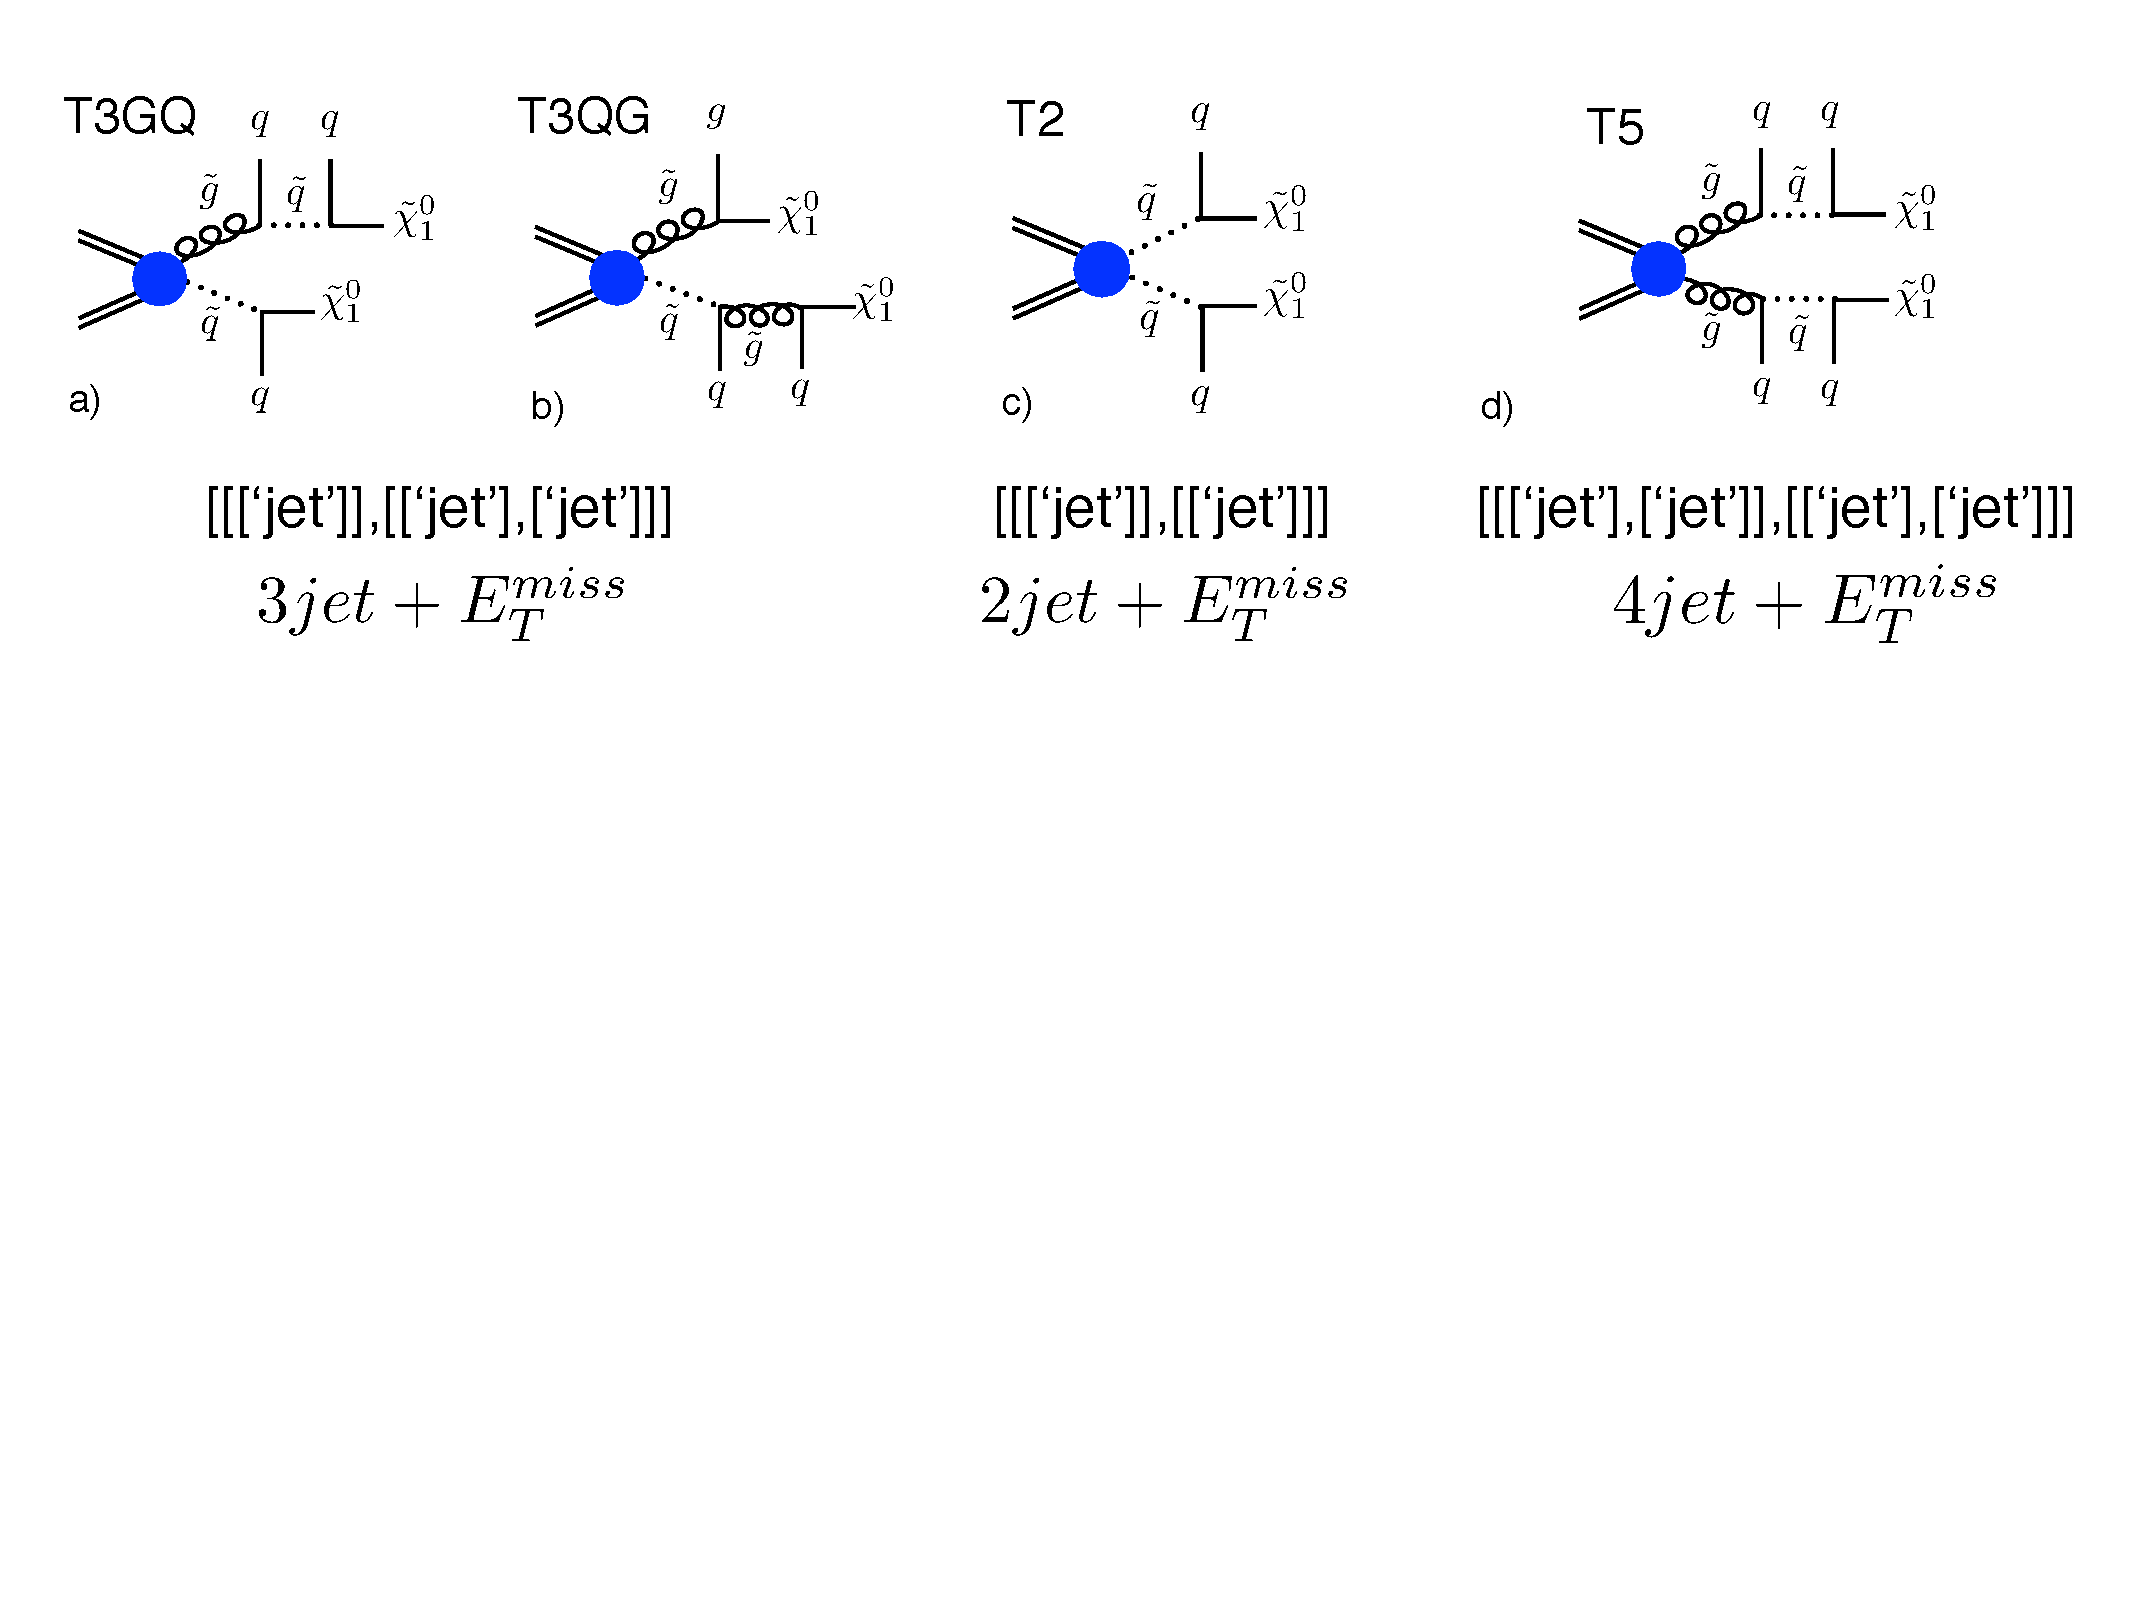
\includegraphics[width=0.9\textwidth]{PLOTS/Diagrams_2}
\end{center}
\caption{Diagrams for the simplified models used for the extension of the database. Models \textit{T3GQ}(a) and \textit{T3QG}(b), corresponding to the two different mass hierarchies $m_{\tilde g} > m_{\tilde q}$ and $m_{\tilde q} > m_{\tilde g}$, are identified by the experimental signature \textit{[[[`jet']],[[`jet'],['jet']]]} in \SMO~notation. Diagrams c) and d) represent the \textit{T2} and \textit{T5} models, mapping to the \textit{[[[`jet']],[['jet']]]} and \textit{[[[`jet'],['jet']],[[`jet'],['jet']]]} signatures.}
\label{Diagrams}
\end{figure*}
%
As stated in the introduction, the \textit{T3GQ} model was foud to be the most important missing result for the pMSSM. It is to note, however that, by construction, the \textit{T2} and \textit{T5} models, represented by plots c) and d) of Fig. \ref{Diagrams}, are automatically important when the \textit{T3GQ} model is. In practice, the \textit{T3GQ} model is an asymmetric model composed by one branch from the \textit{T2} and one branch from the \textit{T5} models. Thanks to the usage of EM results, it is thus possible to combine the signals from the $pp \rightarrow \tilde g \tilde g$, $pp \rightarrow \tilde q \tilde q$ and $pp \rightarrow \tilde g \tilde q$ channels. Along with the results from \textit{TGQ}, the power of combining the \textit{T2} and \textit{T5} models will be explored in this work. For completeness, results for the \textit{T2} and \textit{T5} models were already included in the previous release of the database, hence did not appear in the missing topologies list of the original study.

\section{Description of the Analysis Setup}\label{sec::setup}
In this Section we describe the setups of the Monte Carlo production followed by the analysis recasting for the extraxtion of the efficiency maps, followed by the description of the analysis of the constraints on the pMSSM with simplified models with the \SMO~tool.
\subsection{Production of the Efficiency Maps}
The set-up for the production of the Monte Carlo signals is here described. Events at parton level were generated using \texttt{MadGraph5\_aMC@NLO}\cite{2011uj} , and then showered and hadronized using \texttt{Pythia 6.4}\cite{Sjostrand:2006za}. The processes considered for the production of the samples for the simplified model are described in Tab. \ref{mg5_processes}. All the processes considered the emission of up to one extra parton. The syntax $\$go \ Q$ is used to avoid the presence of on-shell resonances, represented by intermediate gluino and squarks, and double counting when performing the merging between matrix-element and parton-shower.
%
\small
\begin{table}[!]
\begin{center}
\renewcommand{\arraystretch}{1.0}
\begin{tabular}{ l l }  \toprule  \toprule 
%\multicolumn{3}{c}{($M_1,M_2,M_3) = (1000,200,190)$} & \multicolumn{3}{c}{ \textbf{T3GQ}} & \multicolumn{3}{c}{ \textbf{T3QG}} \\  \toprule 
\multicolumn{2}{c}{\texttt{MadGraph5\_aMC@NLO} processes} \\ \toprule \toprule
\multicolumn{2}{l}{\Ttwo: $p p \rightarrow \tilde q \tilde q$}  \\
     & define Q = dl dr dl\textasciitilde dr\textasciitilde ul ur ul \textasciitilde ur\textasciitilde \\
     & generate p p > Q Q  \\
     &  add process p p > Q Q j \\  \toprule 
\multicolumn{2}{l}{\Tfive: $p p \rightarrow \tilde g \tilde g$ } \\ 
     & generate p p > go go \\
     &  add process p p > go go j \\ \toprule 
\multicolumn{2}{l}{\TGQ: $p p \rightarrow \tilde g \tilde q$} \\  
     &  define Q = dl dr dl\textasciitilde dr\textasciitilde ul ur ul\textasciitilde ur\textasciitilde \\
     &  generate p p > go Q \$ go Q \\
     &  add process p p > go Q j \$ go Q \\  \bottomrule \bottomrule 
%
\end{tabular}
\end{center}
\caption{\texttt{MadGraph5\_aMC@NLO} processes for the production of the Monte Carlo samples.}
\label{mg5_processes}
\end{table}
%
The process includes the possiblity of emission of up to one extra parton. The merging between the matrix elements and parton-shower formalisms was performed adopting the $k_T \ jet$ MLM scheme \cite{MLM,Alwall:2007fs}. 
%
The analysis recasting was performed with \texttt{MadAnalysis 5}, using the recasting codes for the analysis ATLAS-SUSY-2013-02\cite{ATLAS-SUSY-2013-02MA5,ATLAS-SUSY-2013-02VALIDATION} and CMS-SUS-13-012\cite{CMS-SUS-13-012MA5,CMS-SUS-13-012VALIDATION}. The tuned version of \texttt{DELPHES 3} integrated in the \texttt{MadAnalysis 5} framework was used to perform the simulate the detector effects on the particle objects. Jets were clustered using \texttt{FastJet}\cite{Cacciari:2011ma}.
%
The description of the grid of mass points defined for the production of the efficiency maps is provided in Tab. \ref{TGQ_Planes}. The analyses chosen for the recasting search for SUSY events in the all hadronic final state, vetoing the presence of isolated leptons. In particular the two above analyses are sensitive to events with small jet multiplicity, as generated by the simplified models considered. Although official EM results for the \textit{T2} model were made public by the collaborations, part of the parameter space with small mass gap between the squark and the LSP is below $~$50 GeV is not properly covered. For this reason, EMs were produced, up to a mass difference as small as 5 GeV between the squarks and the LSP. In addition, also the results for the \Tfive~model were extended to cover scenarios with small mass difference between the gluino-squark and squark-neutralino. The parameter x is defined so that $m_{\tilde q}= x\cdot m_{\tilde g} + (1-x)\cdot m_{\tilde \chi_1 ^0}$. For the \textit{T3GQ} model, the gluino mass reaches the value of 2 TeV, with a binning of 50 GeV for $200 \leq m_{\tilde g} < 1200$, and a binning of 100 GeV for $1200 \leq m_{\tilde g}  \leq 2000$ GeV. {\color{blue} The squark masses have a 50 GeV binning, up to 1 TeV. } For a better coverage of the parameter space in the case of small mass differences, additional mass planes parametrized with $\Delta M ( \tilde q, \tilde \chi _1 ^0)$=(5,10,15) GeV were produced.
%
\begin{table}
\footnotesize

\begin{center}
\renewcommand{\arraystretch}{1.0}
\begin{tabular}{ l l l }  \toprule \toprule 
\multicolumn{3}{c}{\texttt{ \normalsize \textbf{Mass Planes}}} \\ \toprule \toprule
\multicolumn{3}{l}{\Ttwo: $p p \rightarrow \tilde q \tilde q$} \\
     & - & min($\Delta M(\tilde q, \tilde \chi _1 ^0)$) = 5 GeV \\ \midrule
\multicolumn{3}{l}{\Tfive: $p p \rightarrow \tilde g \tilde g$} \\ 
     &x=(0.05,0.50,0.95) &  \\ 
     &$\Delta M(\tilde q, \tilde \chi _1 ^0)$ = 5 GeV&  \\ \midrule
\multicolumn{3}{l}{\TGQ: $p p \rightarrow \tilde g \tilde q$} \\  
     & $m_{\tilde g}$ = 200,...,1200 & 50 GeV bin \\ 
     & $m_{\tilde g}$ = 1300,...,2000 & 100 GeV bin ($m_{\tilde g}\leq$2 TeV) \\
     & $m_{\tilde q}$ & 50 GeV bins ($m_{\tilde q}\leq$1 TeV) \\
     & & min($\Delta M(\tilde q, \tilde \chi _1 ^0)$) = 5 GeV \\ \bottomrule \bottomrule
\end{tabular}
\end{center}
\caption{Mass plane parametrization used for the EMs production of the \textit{T2}, \textit{T3GQ} and \textit{T5}. See the text for details.}
\label{TGQ_Planes} 
\end{table}
%
The mass hierarchy used for the production of the gluino-squark model is $m_{\tilde g} > m_{\tilde q}$, meaning that the \textit{T3GQ} model was chosen to constrain the "[[[`jet']],[[`jet],[`jet']]]" signature. Note that the same problem related to the choice of the mass hierarchy applies to the $T5$ model: the "[[[`jet']],[[`jet']]]" signature can be obtained both with $\tilde g \rightarrow g \tilde \chi _1 ^0$ and $\tilde q \rightarrow q \tilde \chi _1 ^0$; for the maps production, again the former hierachy was chosen. 
%
\subsection{SModelS Analysis}
The setup for the analysis with \SMO~follows closely what described originally in \cite{Ambrogi:2017lov}, that is here summarized. The pMSSM-19 model points considered in the analysis are a subset of the points used by the ATLAS collaboration in the re-intepretation study\cite{Aad:2015baa}, and made availbel on \texttt{HepData}\cite{ATLASpMSSMhepdata}. Since the aim of the previous and current \SMO~analysis is to quantify the coverage of the pMSSM parameters space by means of simplified model results only, only the points that could be excluded by SUSY searches at 8 TeV were analysed, and points excluded by searches for exotic particle like long lived charged states and resonances compatible with a Heavy Higgs boson were not included. This selection reduced the original number of points tested by ATLAS from 103,410 to 38,575 (Bino-like LSP dataset) and from 126,684 to 45,594 (Higgsino-like LSP dataset). This identical dataset is being re-analysed, and the improvement in the coverage thanks to the newly added efficiency maps result tested. 
\\
Version v1.1.1 of \SMO~was employed, so the the Wino-like LSP dataset was not tested, since most of the models included long-lived charginos that cannot be handled by this version of the software.
The \SMO~cross section calculator, which provides a useful interface with \texttt{Pythia 8}(\texttt{v.8.226})\cite{Sjostrand:2014zea}, \texttt{Pythia 6}\cite{Sjostrand:2006za} and \texttt{NLLFast}~\cite{nllfast,Beenakker:1996ch,Kulesza:2008jb,Kulesza:2009kq,Beenakker:2009ha,Beenakker:2011fu,Beenakker:1997ut,Beenakker:2010nq} was used to compute the production cross sections, up to NLO+NLL order for strong production, and LO for electroweak processes; \texttt{Pythia 6}~was instead used for slepton production. The other two relevant parameters selected in the configuration file \texttt{parameters.ini} are the \texttt{sigmacut}= 0.03 fb (controlling the minimum weight, defined as $w = \sigma \times BR$ for each simplified model appearing in the decomposition) and \verb|minmassgap| = 5 GeV, i.e. the minimum mass gap for which the SM products appearing in the decay chain are considered visible.
\\
\section{Extending the pMSSM Coverage}\label{sec::impact}
In this Section we study the improvements in the pMSSM coverage provided by the additional EMs for the \textit{T3GQ} gluino-squark model, in combination with the \textit{T2} and \textit{T5} model. 
\begin{figure}[!]
\begin{center}
\subfigure
{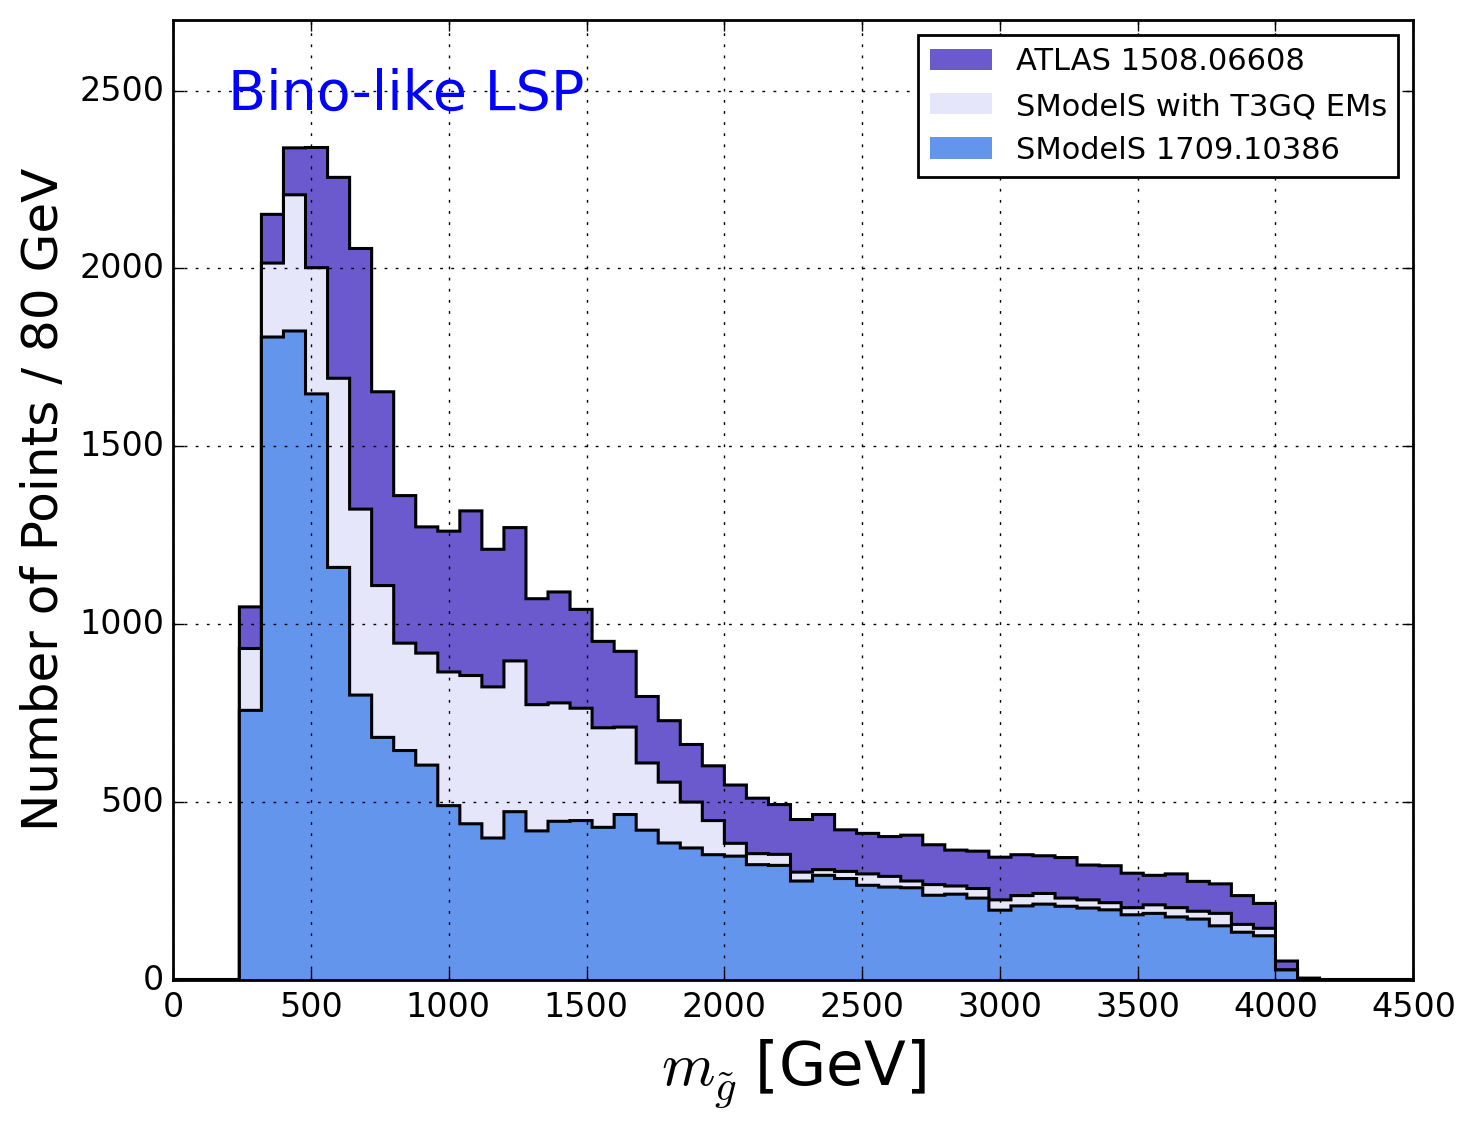
\includegraphics[width=0.49\textwidth]{PLOTS/BINO_Comparison_Gluino.png}}
\subfigure
{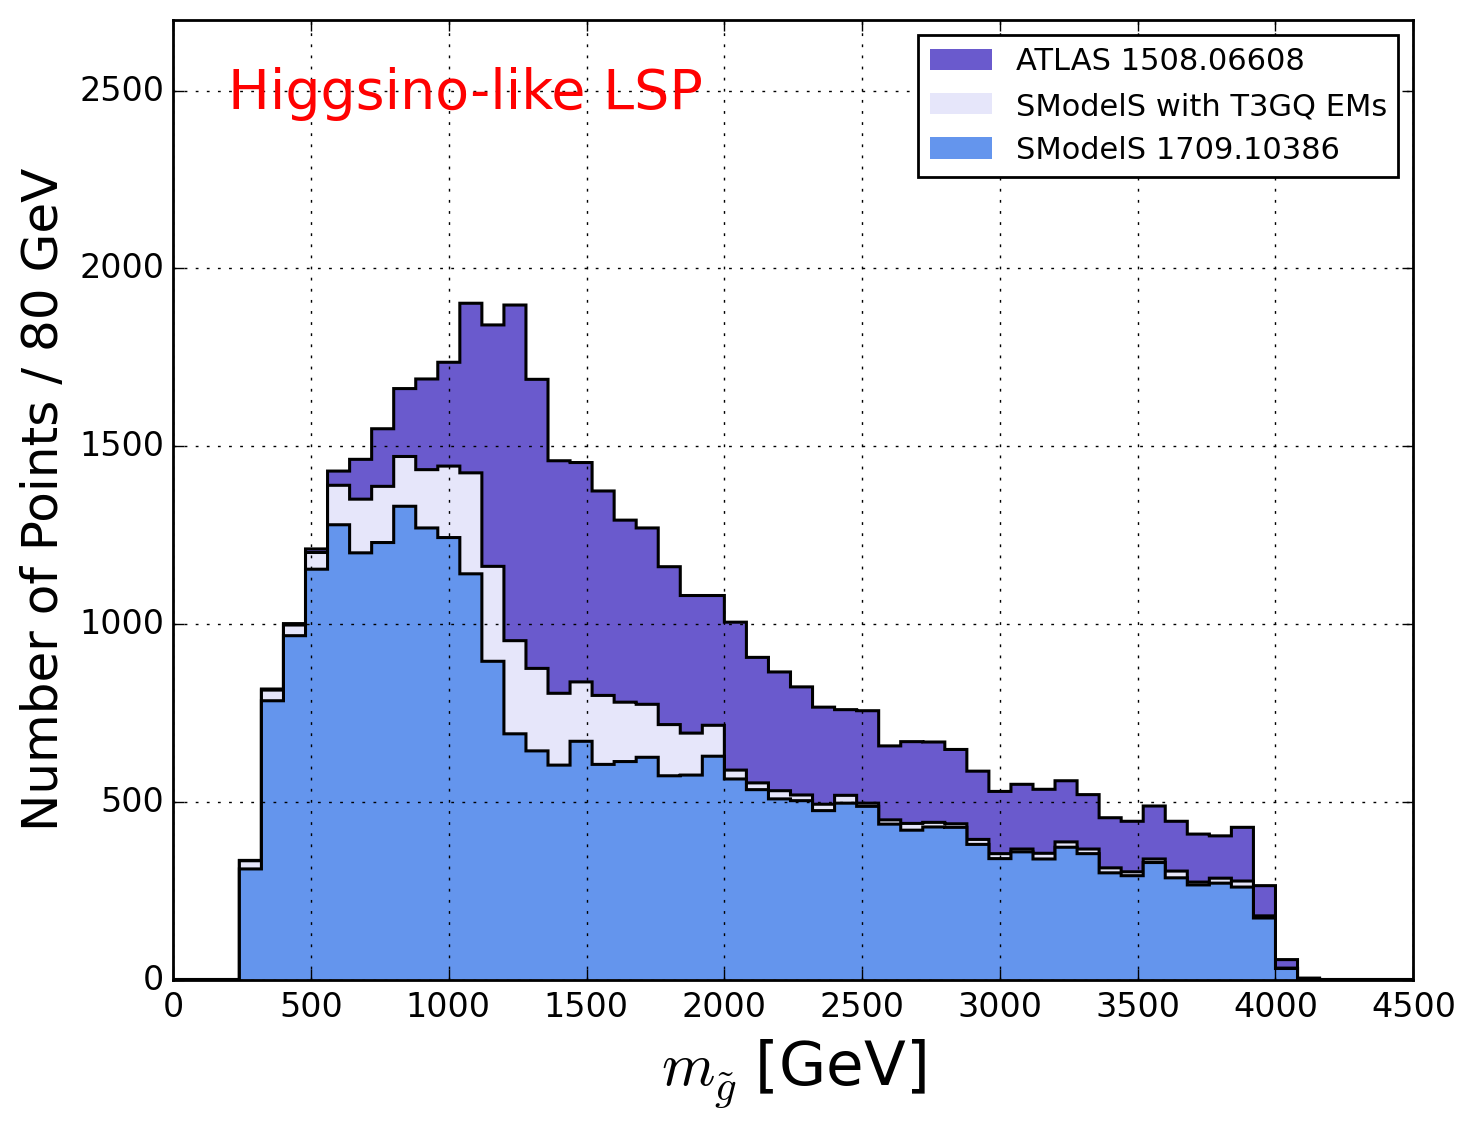
\includegraphics[width=0.49\textwidth]{PLOTS/HIGGSINO_Comparison_Gluino.png}}
\end{center}
\caption{Distributions of the points excluded by ATLAS (purple), by \SMO with the inclusion of the newly `homegrown' maps (light blue), and by the preivous work \cite{Ambrogi:2017lov} (slate blue), for the Bino(top) and Higgsino-like LSP (bottom).}
\label{pmssm_new_exclusion_gluino}
\end{figure}
\begin{table}[!]
\footnotesize
\begin{center}
\renewcommand{\arraystretch}{1.0}
\begin{tabular}{l l c }  \toprule  \toprule 
& \textbf{Total} & \textbf{Excluded (EM+UL)} \\ \toprule \toprule 
\textbf{Bino LSP} & &  \\
     & 38527 & 28765 (74 $\% $) \\ 
\textbf{Higgsino LSP} & &   \\
     & 45345 & 32358 (71 $\% $) \\ \bottomrule   \bottomrule  
\end{tabular}
\end{center}
\caption{SModelS constraints for the Bino and Higgsino-like LSP after the addition of the newly implemented EMs results fro the models \textit{T2}, \textit{T5} and \textit{T3GQ}.}
\label{Res_Tab_New}
\end{table}
%
Table \ref{Res_Tab_New} shows the new total exclusion of the pMSSM points, 21,151 and 28,669 points for the Bino and Higgsino-like case, allowing to cover the 74 and 71 $\%$ of the total points tested. With respect to the previous coverage detailed in \cite{Ambrogi:2017lov}, an improvement in the coverage of +19$\%$ and +8$\%$ respectively is obtained.
%
The major improvement appears in the Bino-like LSP case, as noticeable also in the gluino and squark mass coverage distributions in Fig. \ref{pmssm_new_exclusion_gluino}. Due to the choice of the parametrisation of the mass planes for the sample productin, the bulk of the improvement is found for $m_{\tilde g}\leq$ 2 TeV. The extension of the EM to cover of the small mass gaps between the squarks and the LSP, as described in Tab. \ref{TGQ_Planes}, gives important contribution to the exclusion not only for large gluino masses, but also for intermediate to low mass values.
\begin{figure}[!]
\begin{center}
\subfigure
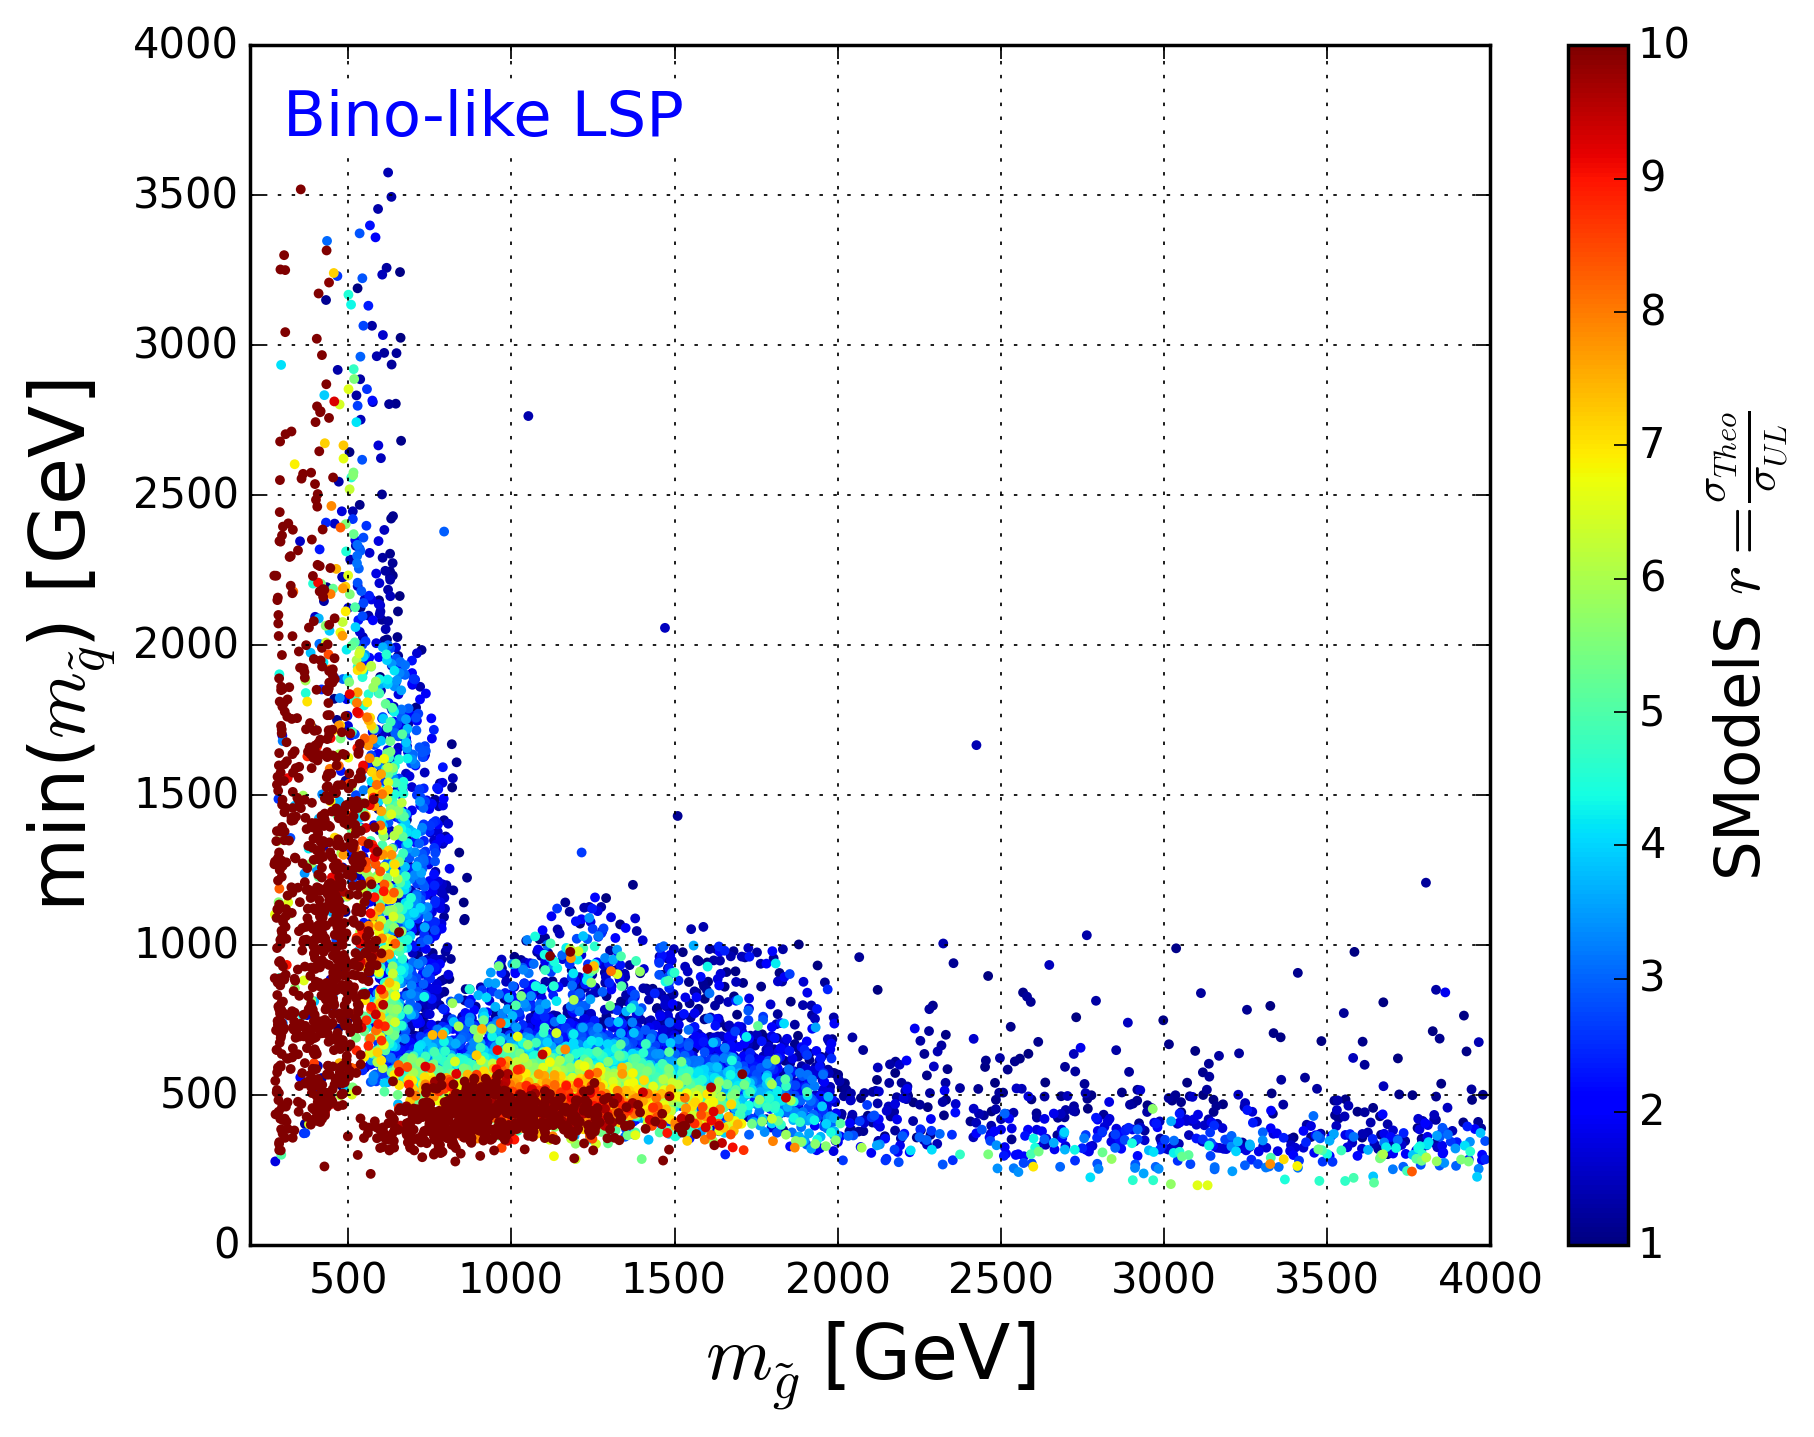
\includegraphics[width=0.49\textwidth]{PLOTS/BINO_rValus_Glu_Sq.png}
\subfigure
{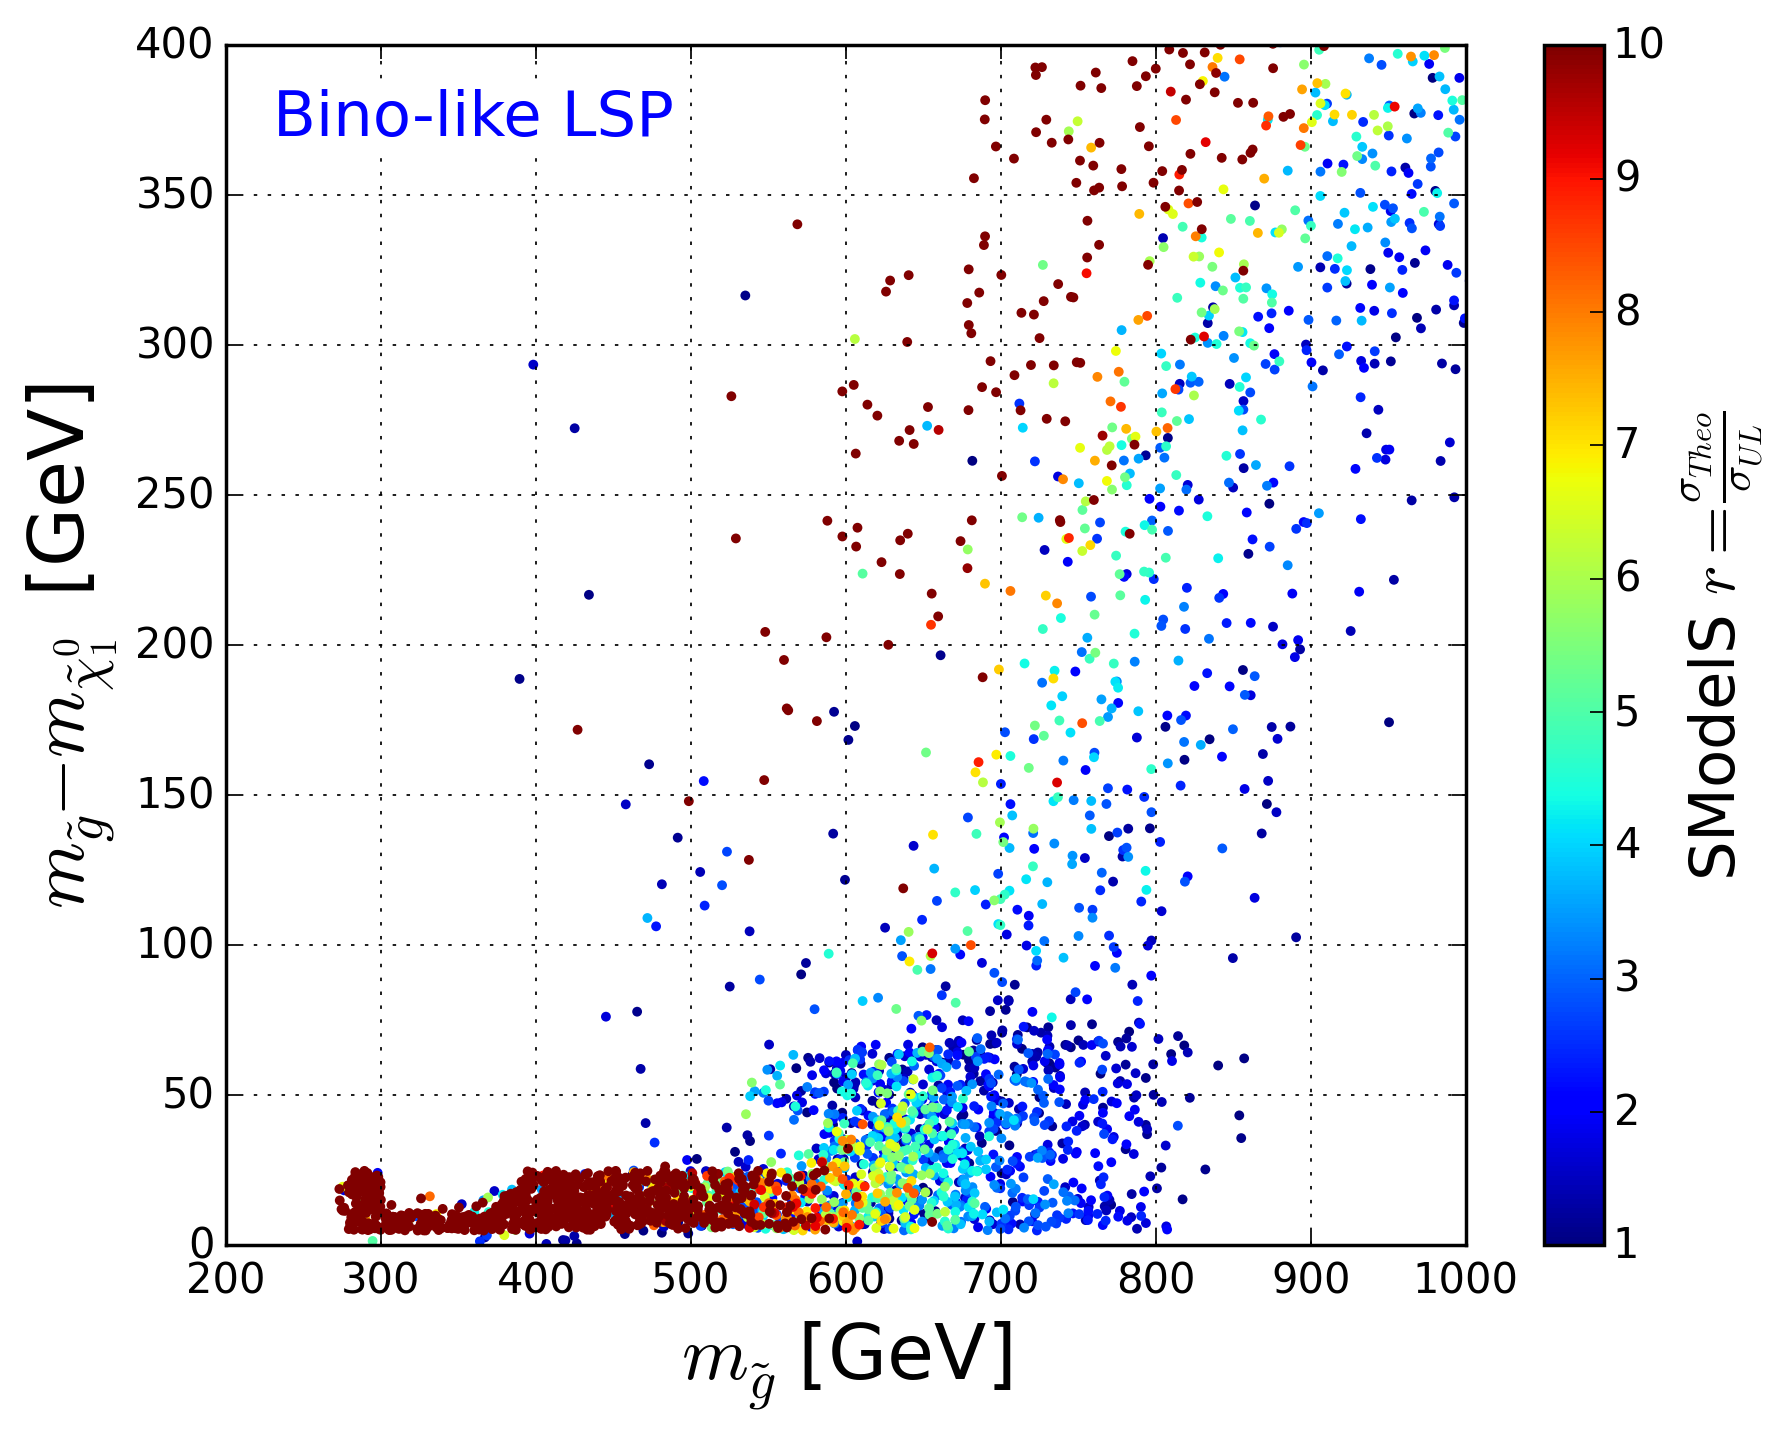
\includegraphics[width=0.49\textwidth]{PLOTS/BINO_rValus_Glu_Diff_Neu.png}}
\end{center}
\caption{\SMO~r-values for the points excluded by the newly implemented EM results, for the Bino-like LSP in the $(m_{\tilde{g}},min(m_{\tilde q})$ and $(m_{\tilde{g}}, m_{\tilde{g}} - m_{\tilde \chi _1 ^0 })$ mass planes (bottom).} 
\label{rValues}
\end{figure}
This can be understood by looking at Fig. \ref{rValues}, that reports in color code the total \SMO rvalue for the Bino-like LSP dataset, for the additionaly excluded points with respect to the previous study (i.e. excluded by the new EM results). The results are projected in the two mass planes $(m_{\tilde{g}},min(m_{\tilde q})$ and $(m_{\tilde{g}}, m_{\tilde{g}} - m_{\tilde \chi _1 ^0 })$. While as a general consideration it can be noticed in both projections that many points exhibit a large rvalue, exceeding the red limit of the color bar of the plot, this become more evident by looking at the plot that focusses on the small mass gap between the gluinos and the LSP. 
\\
%\begin{figure*}[!]
%\begin{center}
%\subfigure
%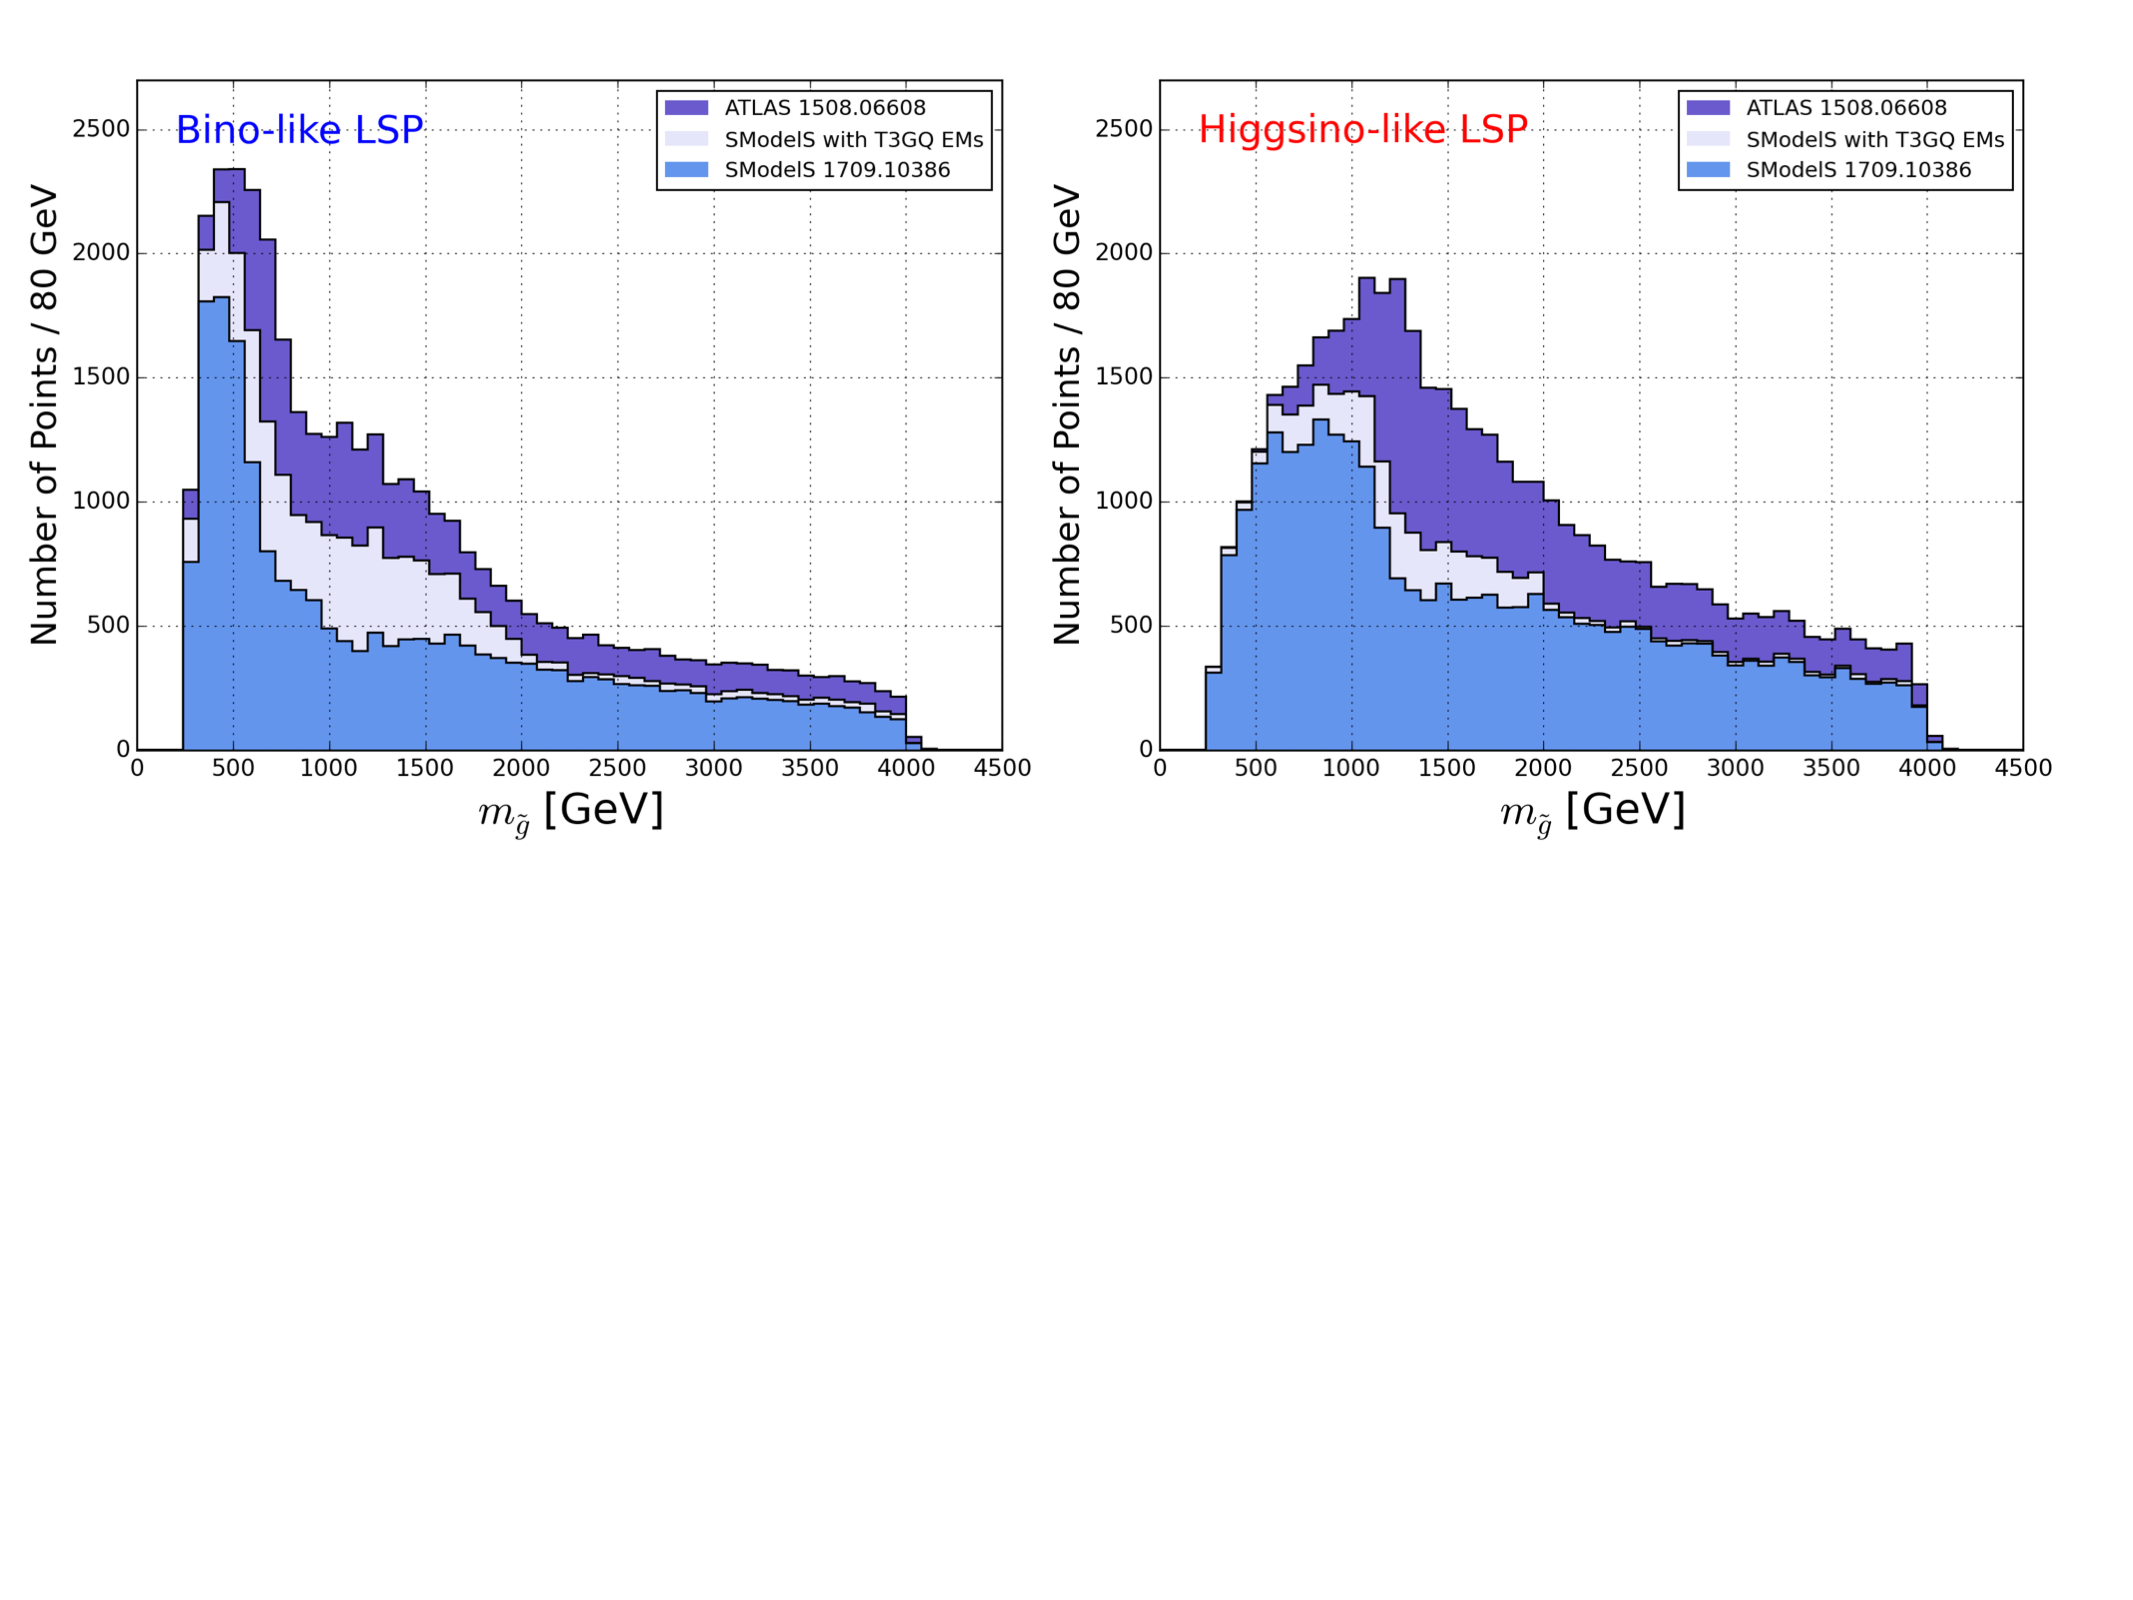
\includegraphics[width=1\textwidth]{PLOTS/New/New-Exclusion.pdf}
%\end{center}
%\caption{} 
%\label{pmssm_new_exclusion_gluino}
%\end{figure*}
%
%
%\begin{figure}[!]
%\begin{center}
%\subfigure
%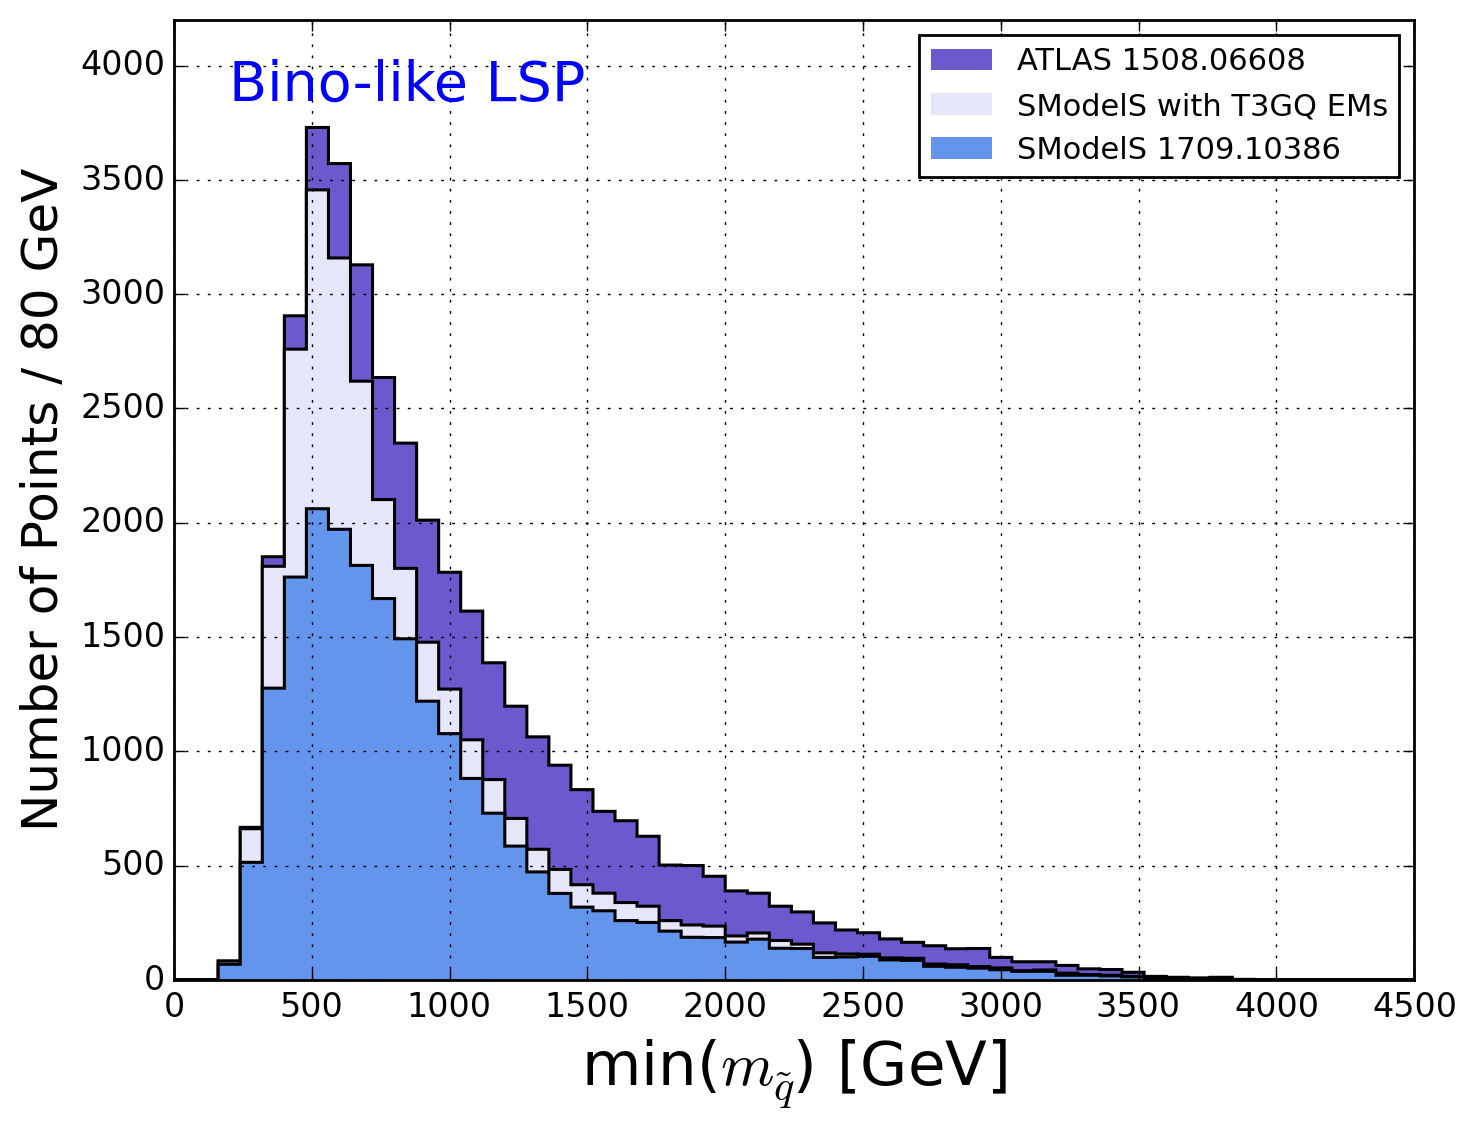
\includegraphics[width=0.49\textwidth]{PLOTS/BINO_Comparison_Sq.png}
%\subfigure
%{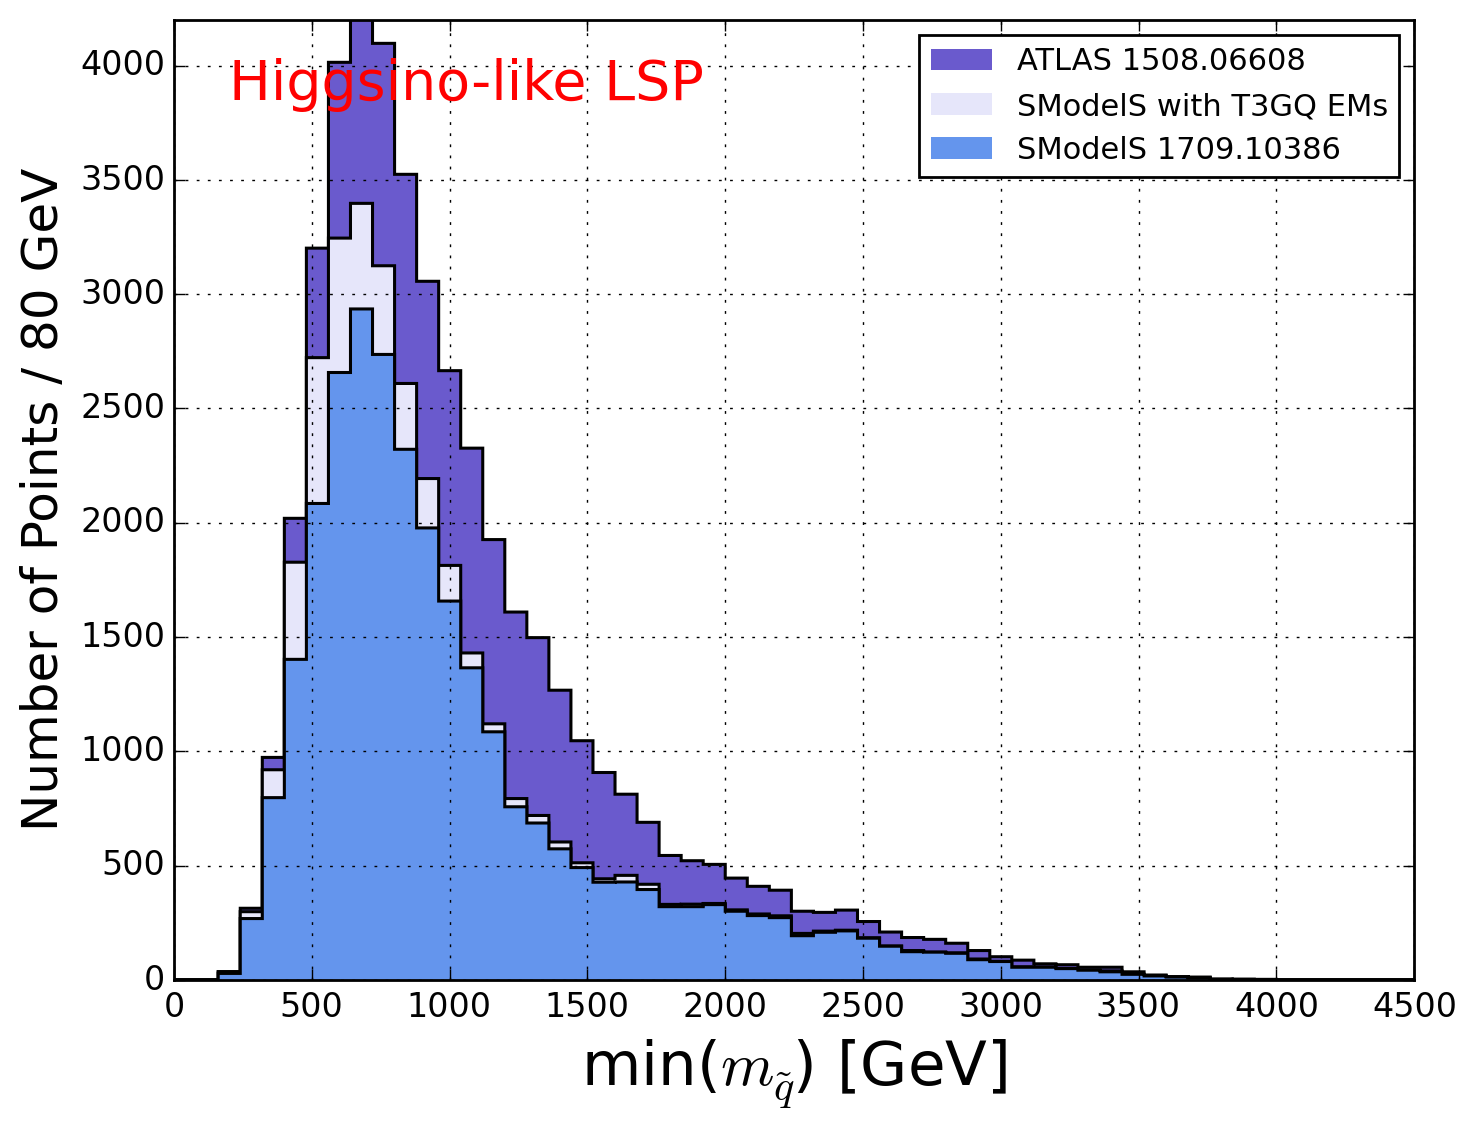
\includegraphics[width=0.49\textwidth]{PLOTS/HIGGSINO_Comparison_Sq.png}}
%\end{center}
%\caption{Same as Fig. \ref{pmssm_new_exclusion_gluino} as a function of \MSQ.} 
%\label{pmssm_new_exclusion_squark}
%\end{figure}
%
%\begin{figure}[!]
%\begin{center}
%\subfigure
%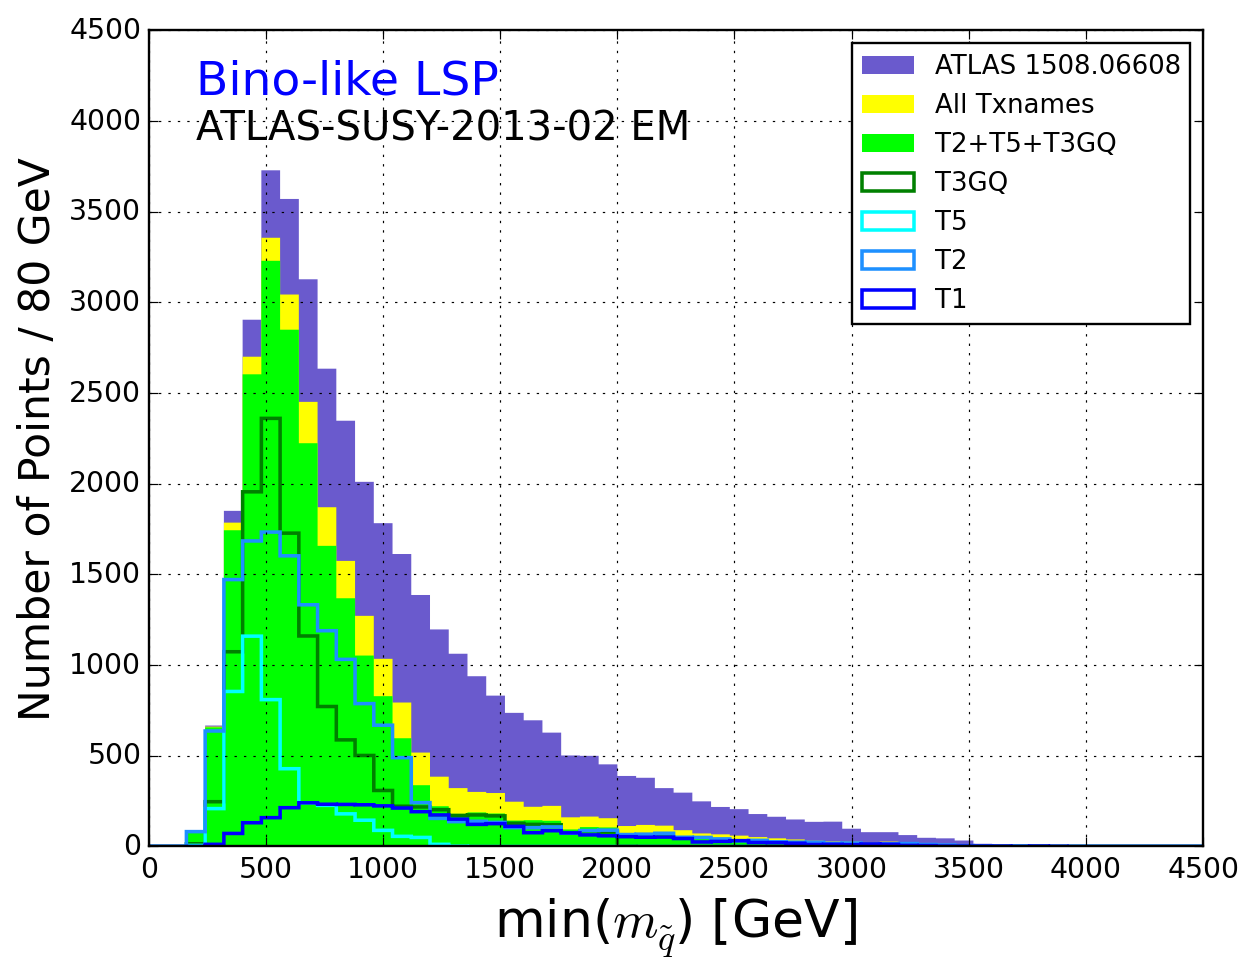
\includegraphics[width=0.49\textwidth]{PLOTS/BINO_Txnames_Contribution_ATLAS02_Squark.png}
%%\subfigure
%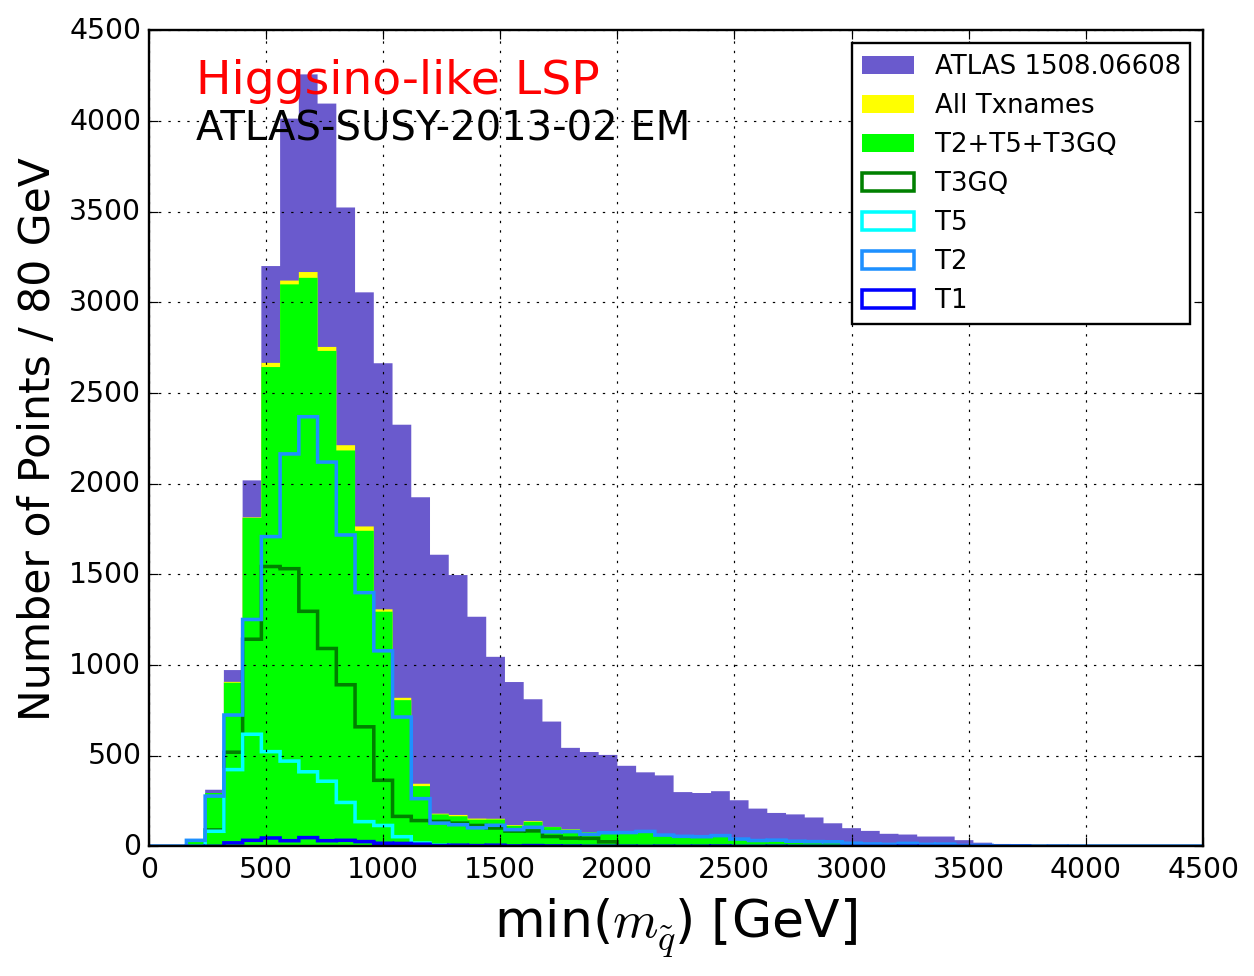
\includegraphics[width=0.49\textwidth]{PLOTS/HIGGSINO_Txnames_Contribution_ATLAS02_Squark.png}
%\end{center}
%\caption{Same as Fig. \ref{combination_gluino} as a function of \MSQ.} 
%\label{combination_squark}
%\end{figure}
%
%\begin{figure}[!]
%\begin{center}
%\subfigure
%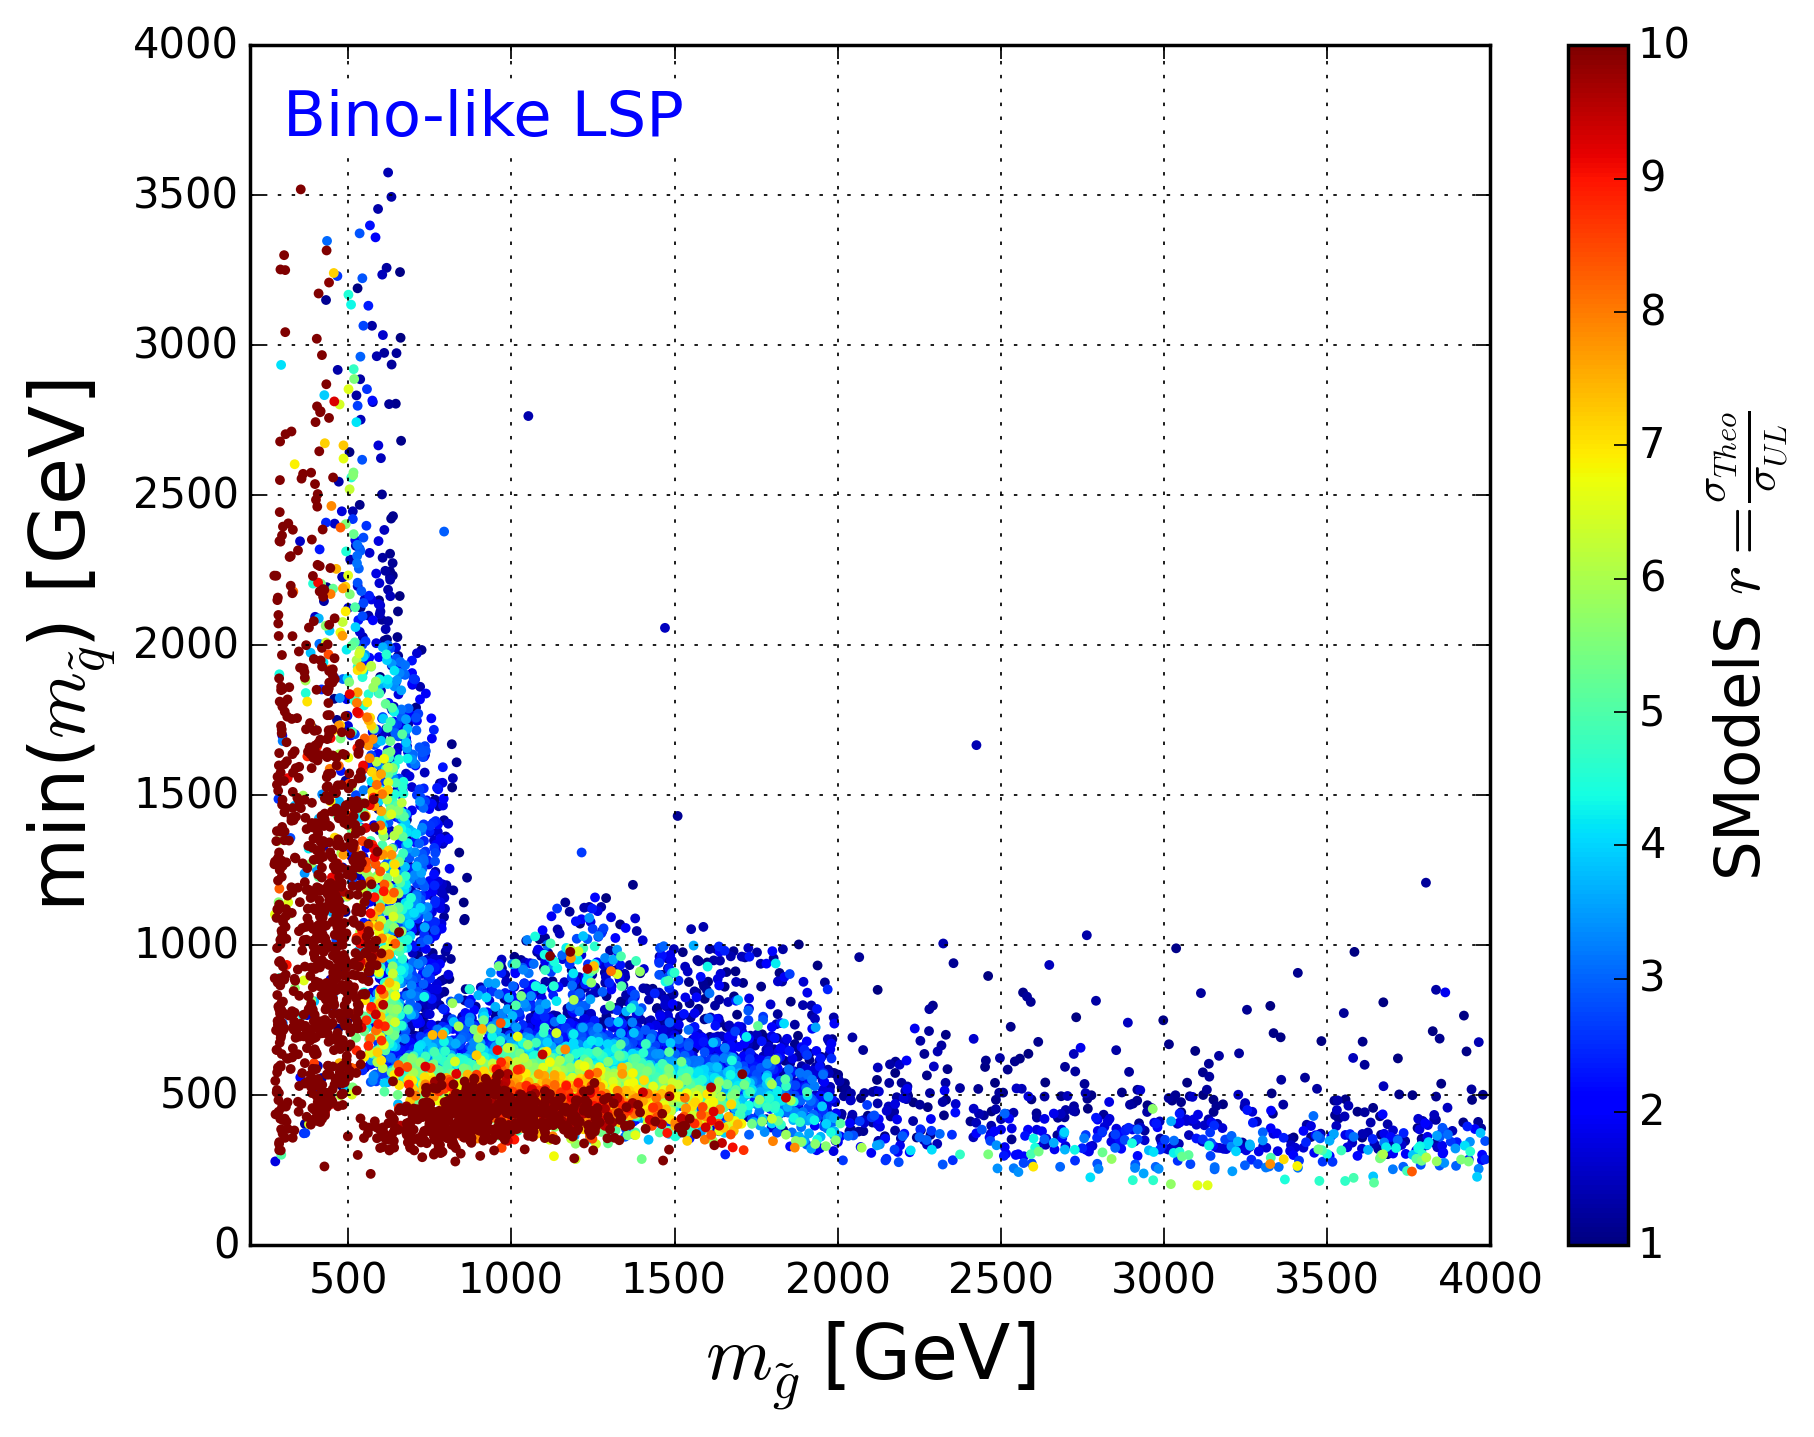
\includegraphics[width=0.49\textwidth]{PLOTS/BINO_rValus_Glu_Sq.png}
%\subfigure
%{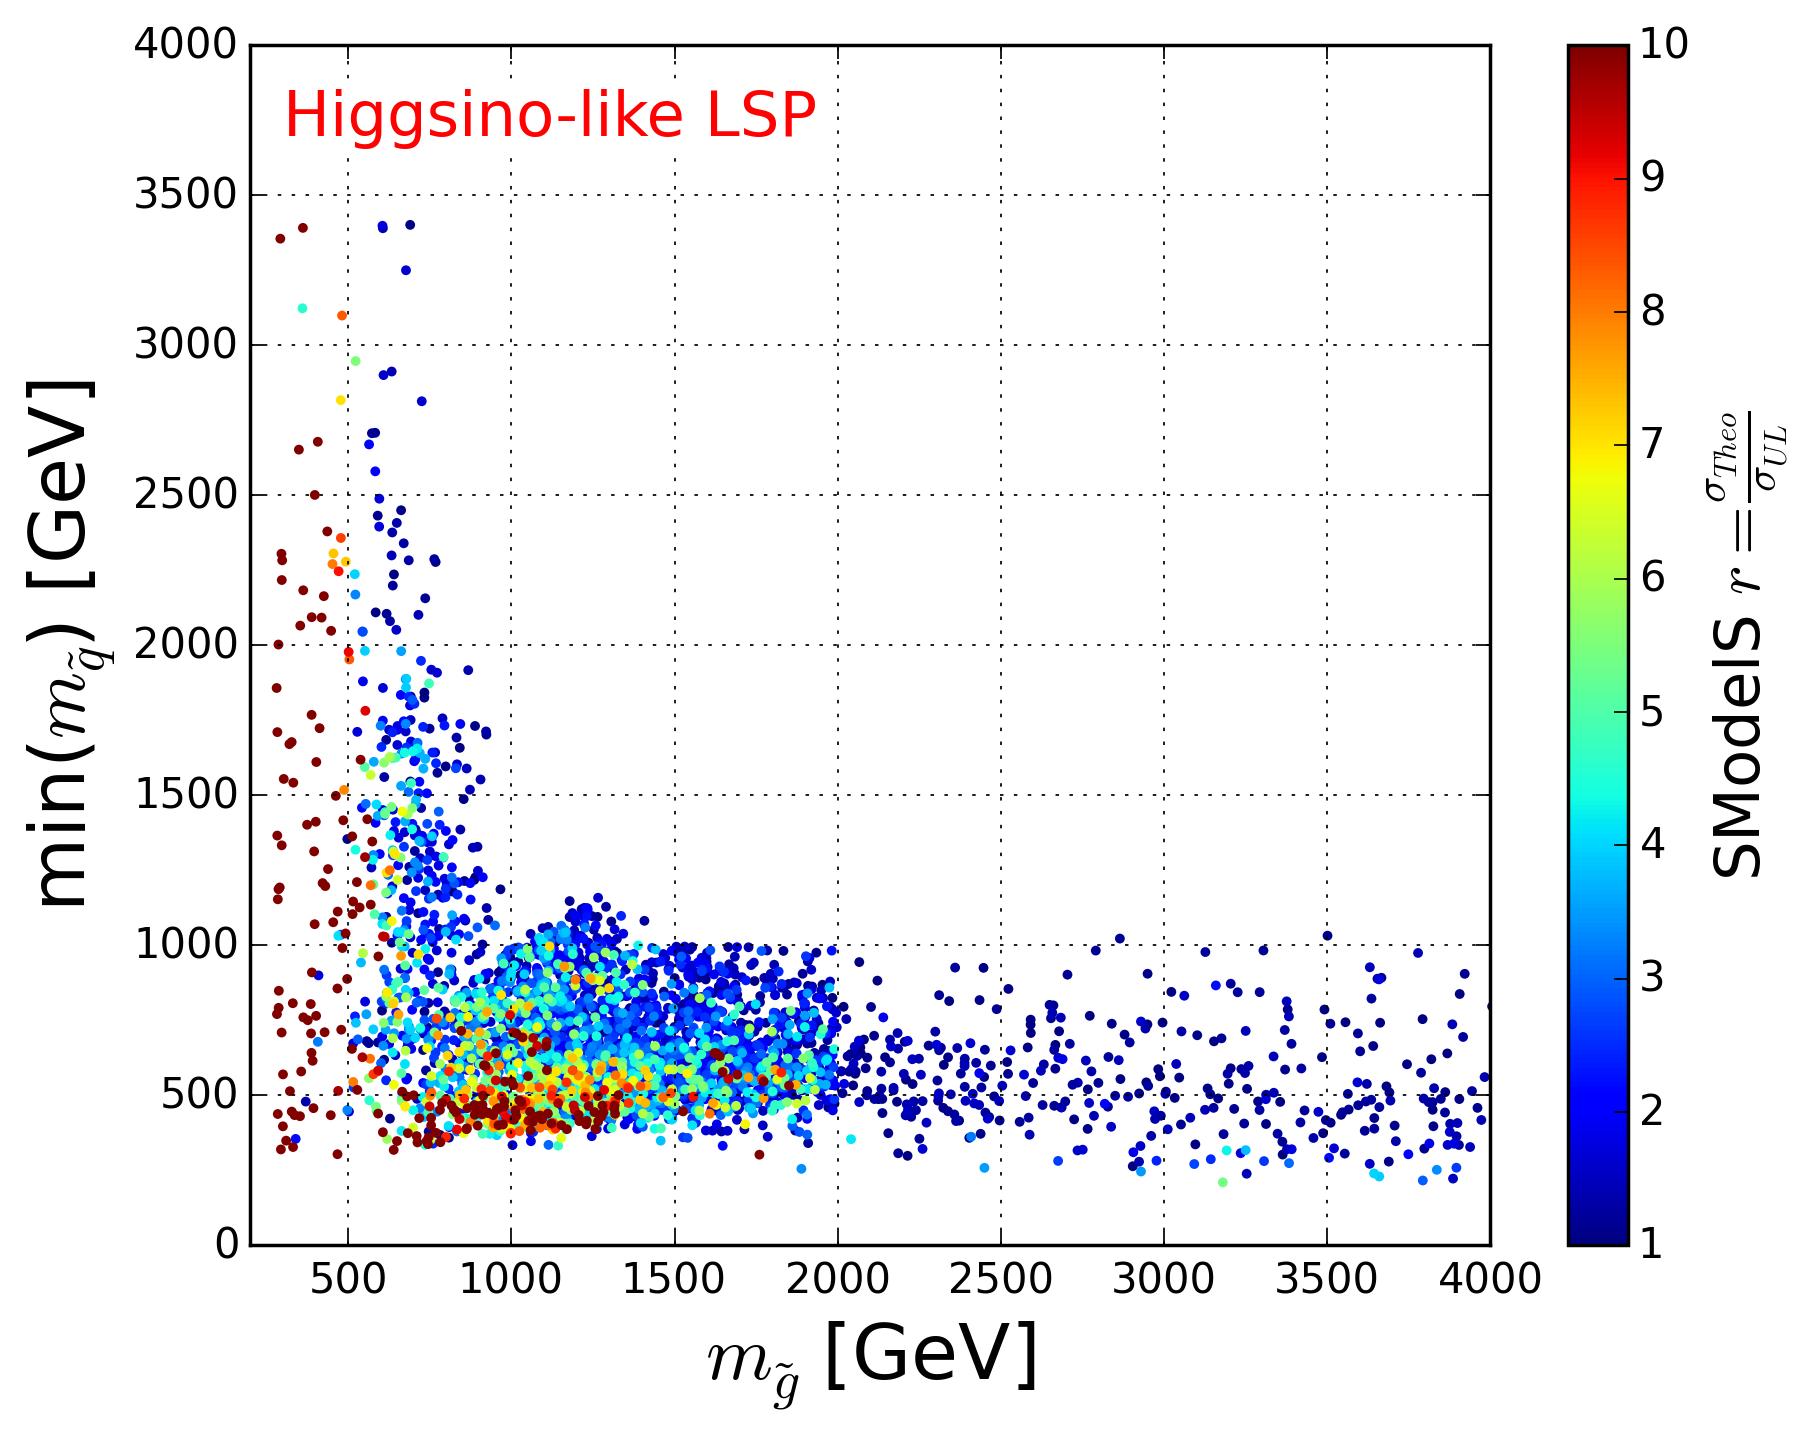
\includegraphics[width=0.49\textwidth]{PLOTS/HIGGSINO_rValus_Glu_Sq.png}}
%\end{center}
%\caption{\SMO~r-values for the points excluded by the newly implemented EM results, for the Bino (left) and Higgsino-like LSP (right).} 
%\label{rValues}
%\end{figure}
%
%\begin{figure}
%\begin{center}
%\subfigure
%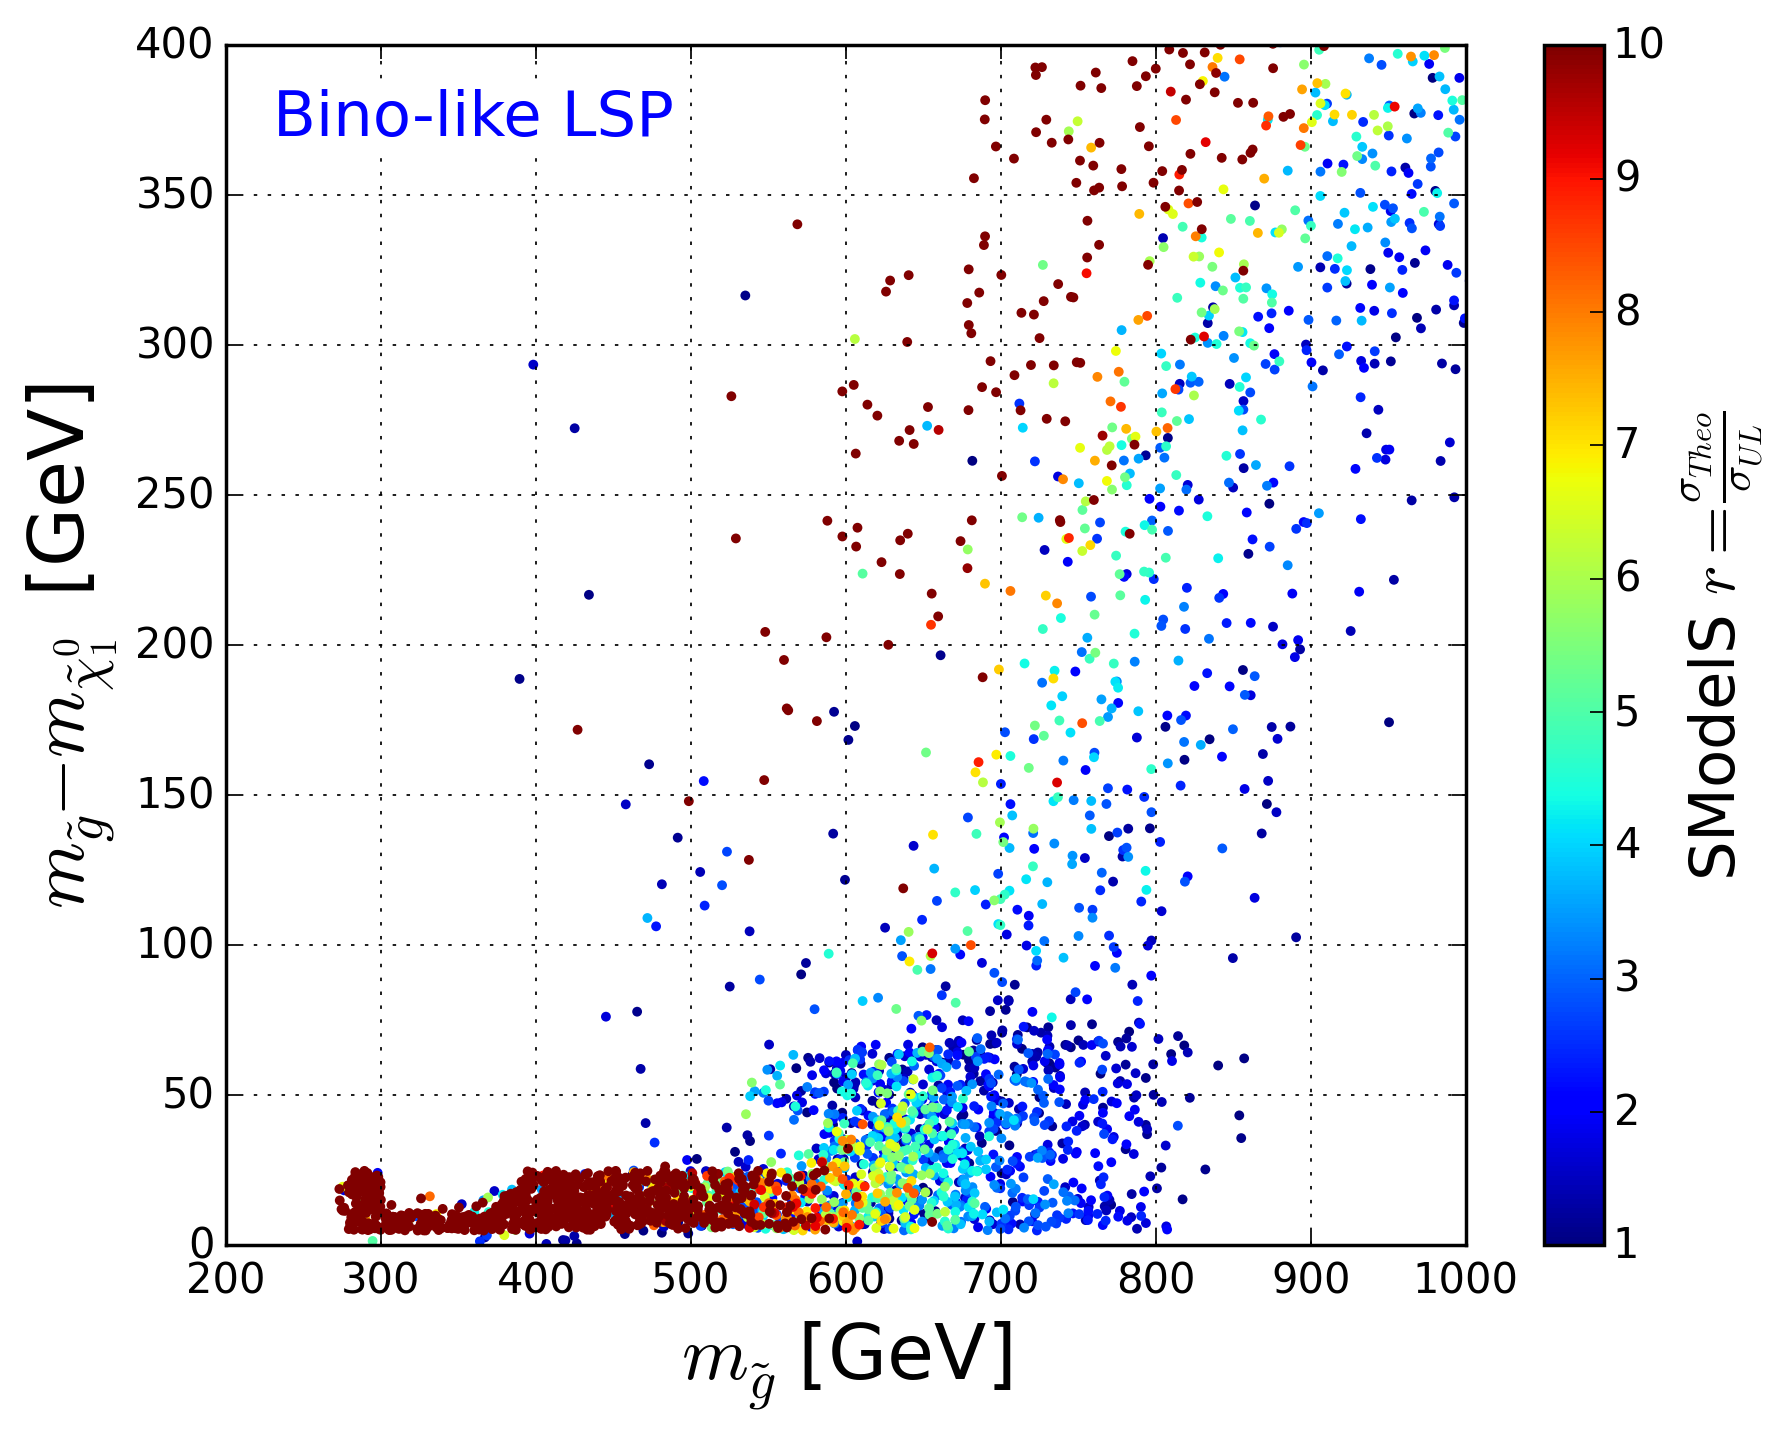
\includegraphics[width=0.49\textwidth]{PLOTS/BINO_rValus_Glu_Diff_Neu.png}
%\subfigure
%{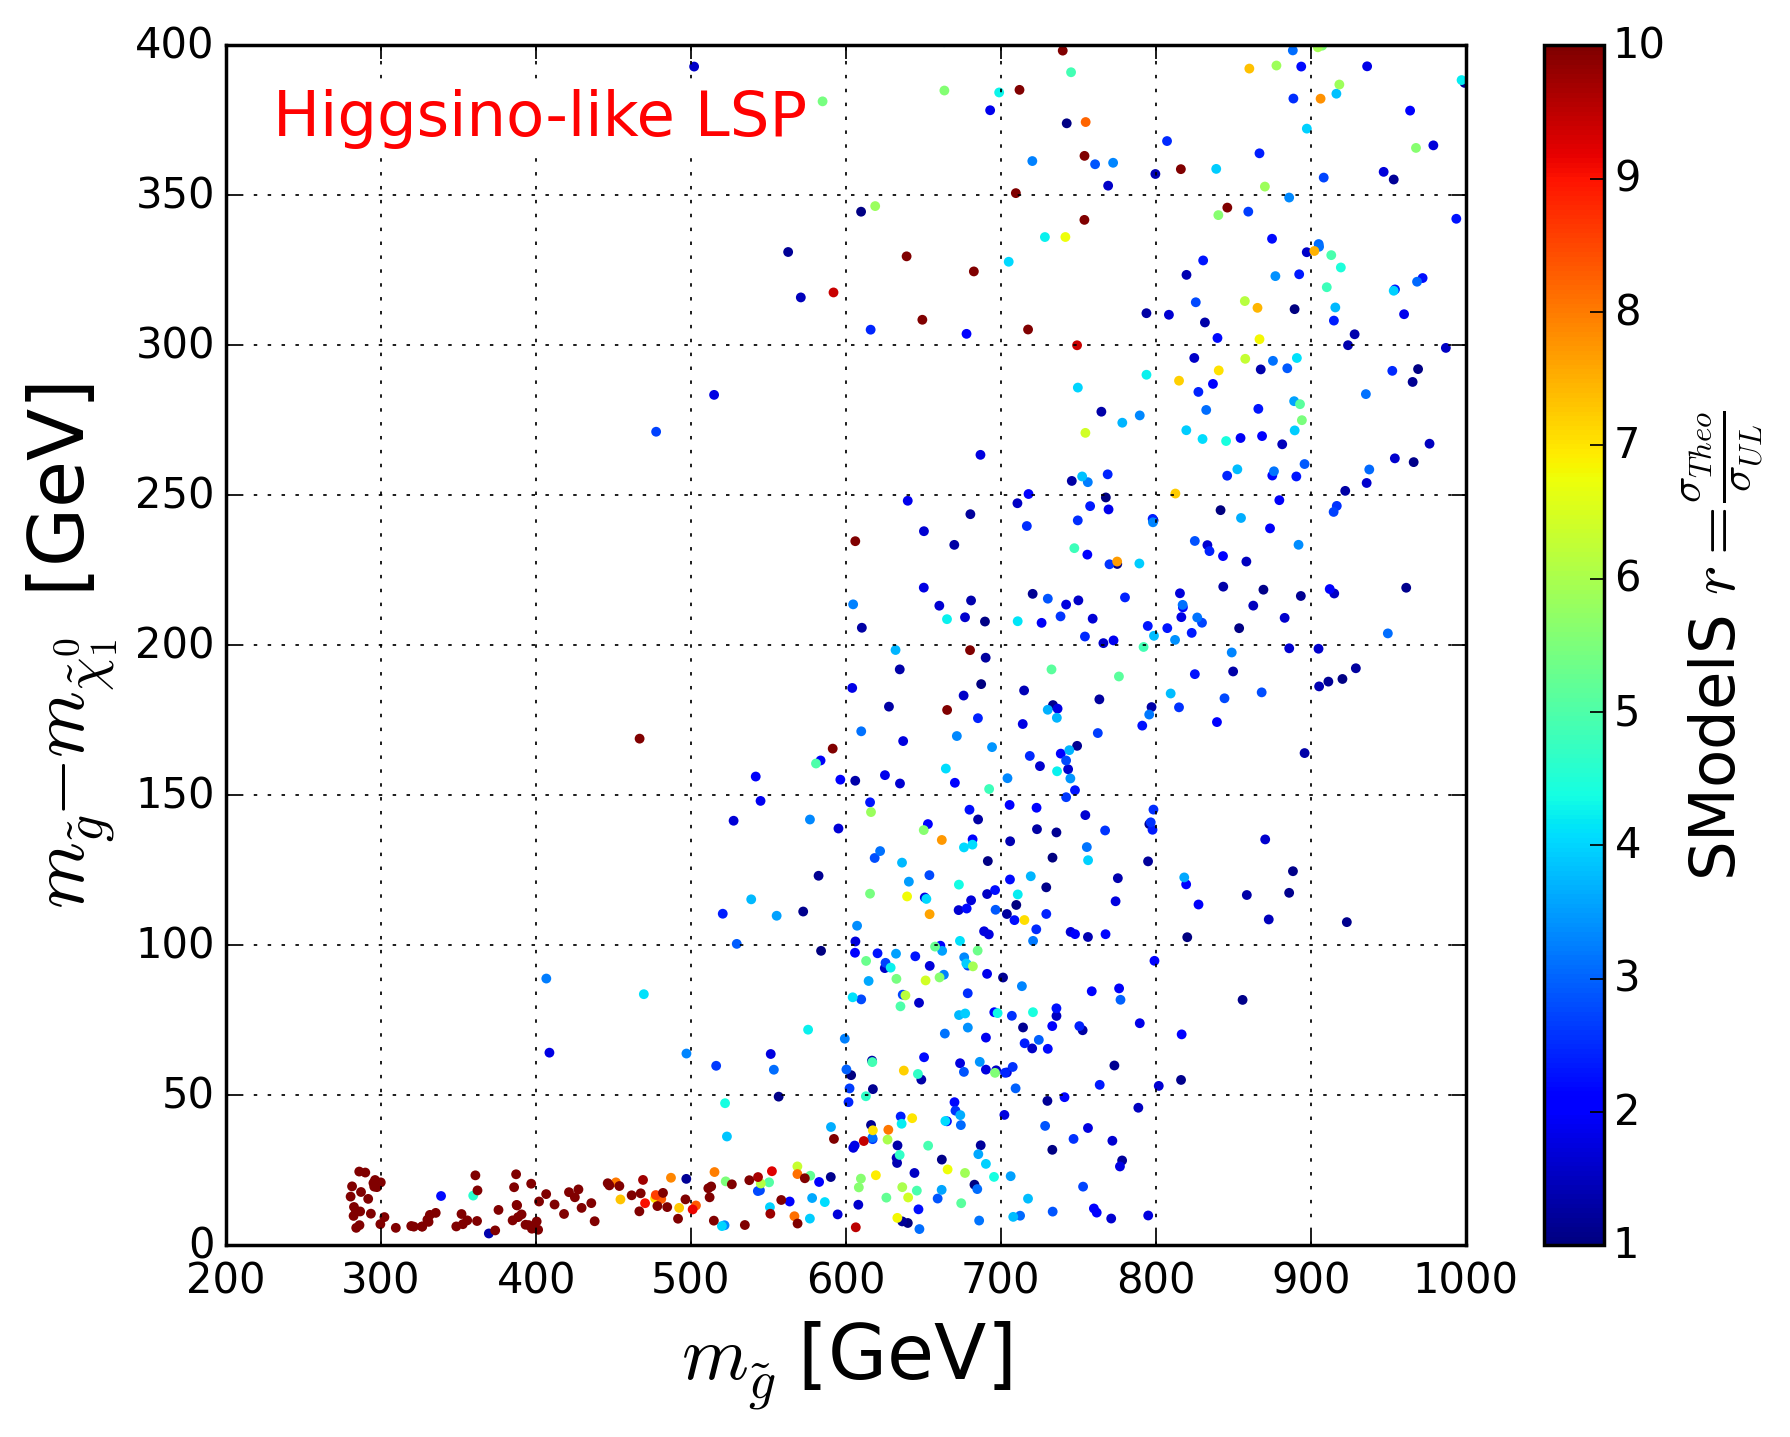
\includegraphics[width=0.49\textwidth]{PLOTS/HIGGSINO_rValus_Glu_Diff_Neu.png}}
%\end{center}
%\caption{\SMO~r-values for the points excluded by the newly implemented EM results. Note the small gap between the lightest squark and the LSP masses. } 
%\label{rValues_diff}
%\end{figure}
%
\subsection{Breakdown of the Results form the different SMS}
As detailed in Section \ref{sec::T3GQ}, the \textit{T2}, \textit{T5} and \textit{T3GQ} can be combined to reconstruct more comprehensively the signals from $\tilde g \tilde g$, $\tilde q \tilde q$ and $\tilde g \tilde q$ production channels. Here we wish to analyse how the newly excluded points benefit from such combination. We limit ourselves to consider only the analysis ATLAS-SUSY-2013-02; together with the recast results, EMs for the \textit{T1} model 
\begin{equation}
p p \rightarrow \tilde g \tilde g , \tilde g \rightarrow q \bar q \tilde \chi_1 ^0
\end{equation}
provided by the ATLAS collaboration are used. The exclusion provided by each model and by the combination of the $T2+T5+T3GQ$ are drawn in Fig. \ref{combination_gluino}. 
%
\begin{figure}[!]
\begin{center}
\subfigure
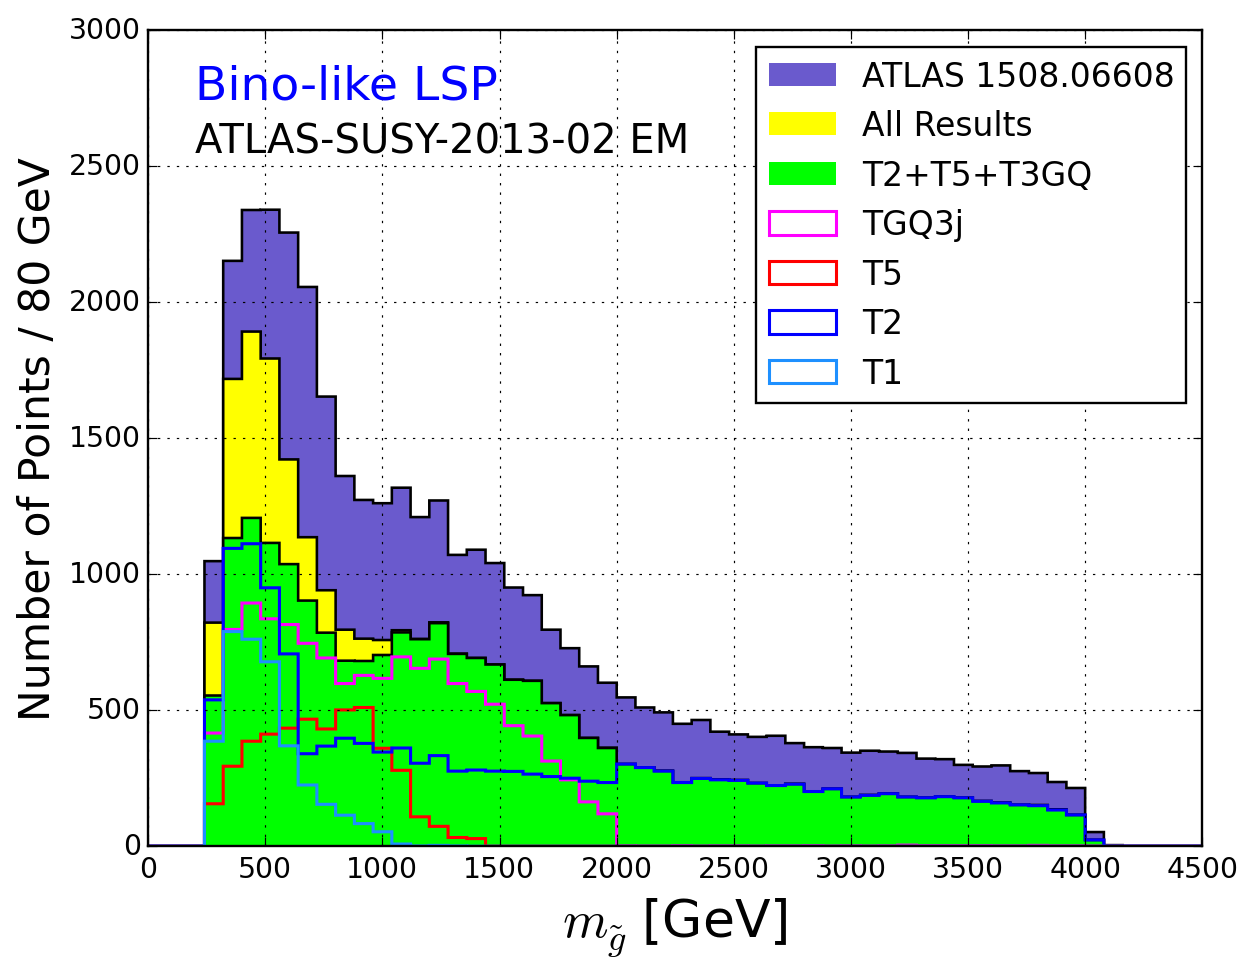
\includegraphics[width=0.49\textwidth]{PLOTS/Combination/BINO_Txnames_Contribution_ATLAS02_Gluino.png}
\subfigure
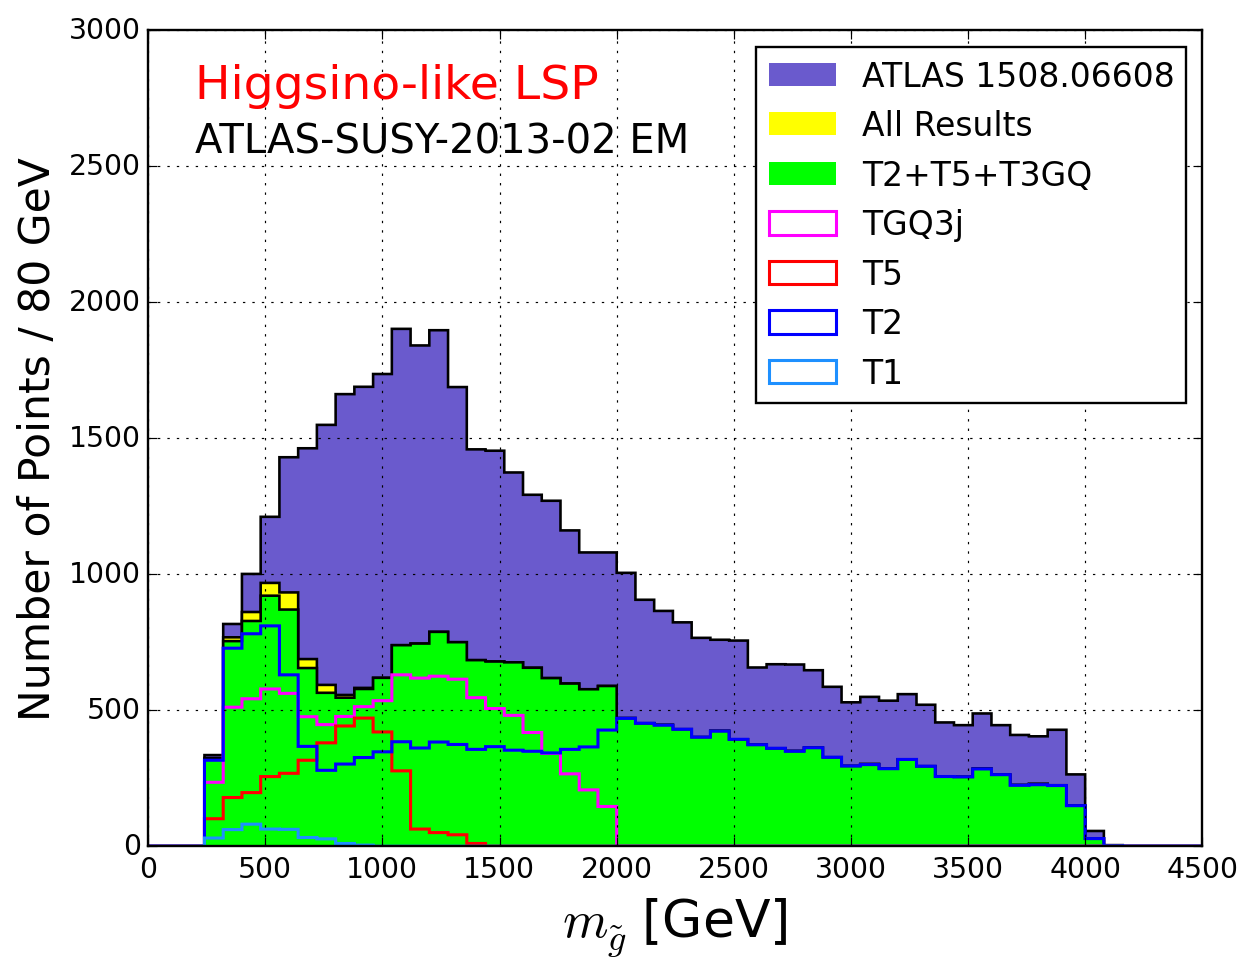
\includegraphics[width=0.49\textwidth]{PLOTS/Combination/HIGGSINO_Txnames_Contribution_ATLAS02_Gluino.png}
\end{center}
\caption{Contribution of the \textit{T1}, \textit{T2}, \textit{T5} and \textit{T3GQ} simplified model results and their combination for the analysis ATLAS-SUSY-2013-02, as a function of \MGLU.} 
\label{combination_gluino}
\end{figure}
%
Note that points can be excluded by more than one results, e.g. points with both light squarks and gluinos, with $m_{\tilde g} > m_{\tilde q}$, might be excluded by both the \textit{T2} and \textit{T5} results; for this reason, the histogram relative to each SMS cannot be stacked together. A major difference between the Bino and the Higgsino-like LSP case concerns the exclusion from the \textit{T1} results, which are significant in the former case, but almost irrelevant in the latter. The model is considered for completeness since such result is available. However, this signal cannot be in general combined with the other signatures of interest, since the \textit{T1} model arises most frequently from the decay of a gluino decaying to an off-shell squark, which is by construction a competing decay channel with respect to the \textit{T3GQ} model. Other SUSY configuration can still result in the \textit{T1} signature, for example the production of charginos and neutralinos decaying hadronically to off-shell vector bosons, but they are practically irrelevant due to the small $\sigma \times BR$.  
\\
In Fig. \ref{rValues} the contribution of the model carrying the highest rvalue among the available \textit{T1}, \textit{T2}, \textit{T5} and \textit{T3GQ} is highlighted. 
\begin{figure}[!]
\begin{center}
\subfigure
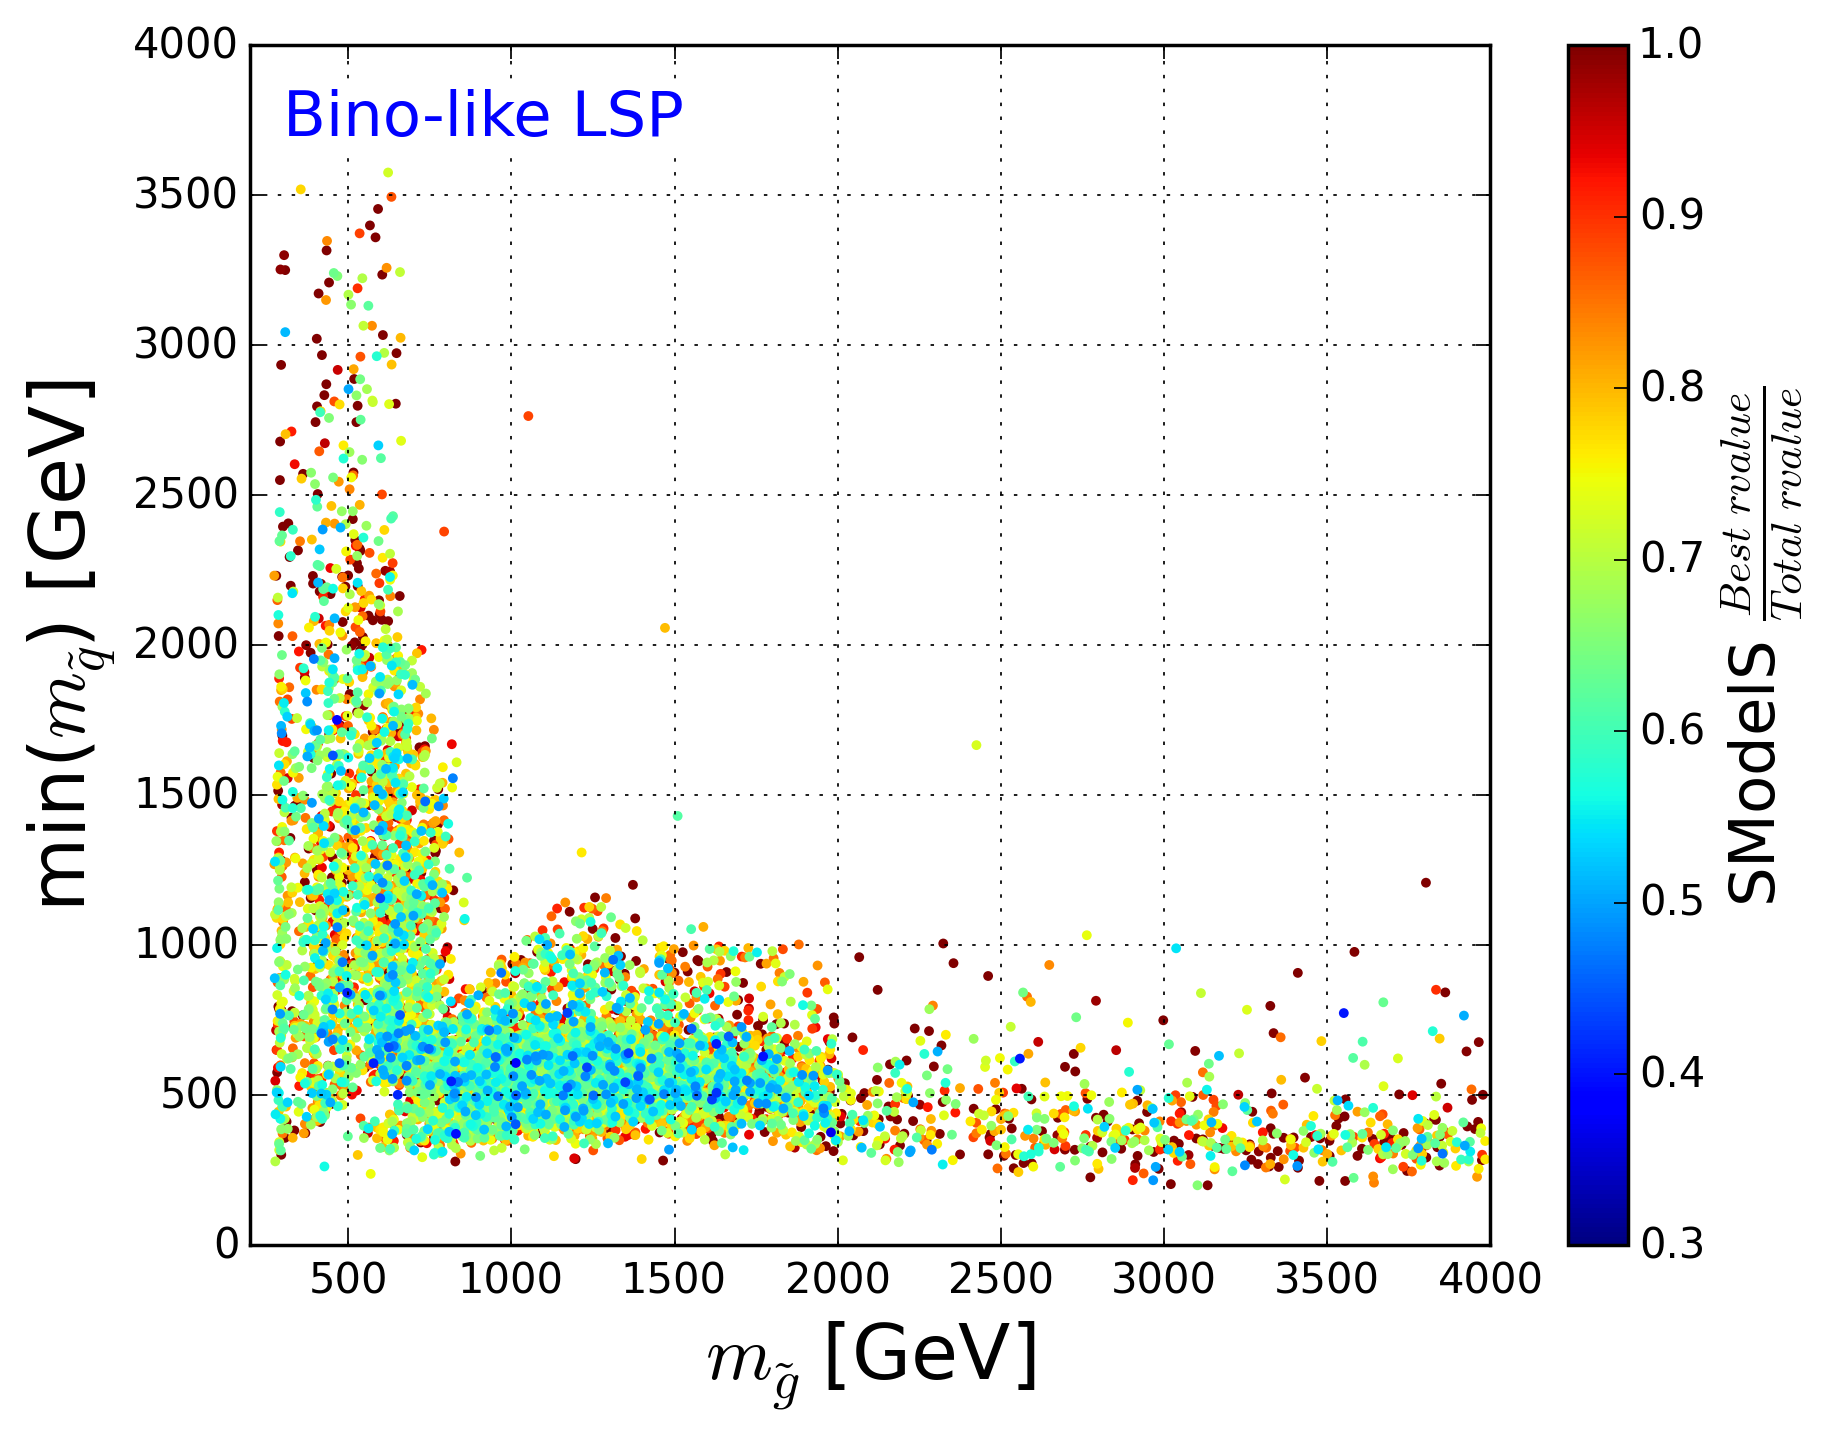
\includegraphics[width=0.49\textwidth]{PLOTS/Weights/BINO_rValus_Glu_Sq_Ratio.png}
\subfigure
{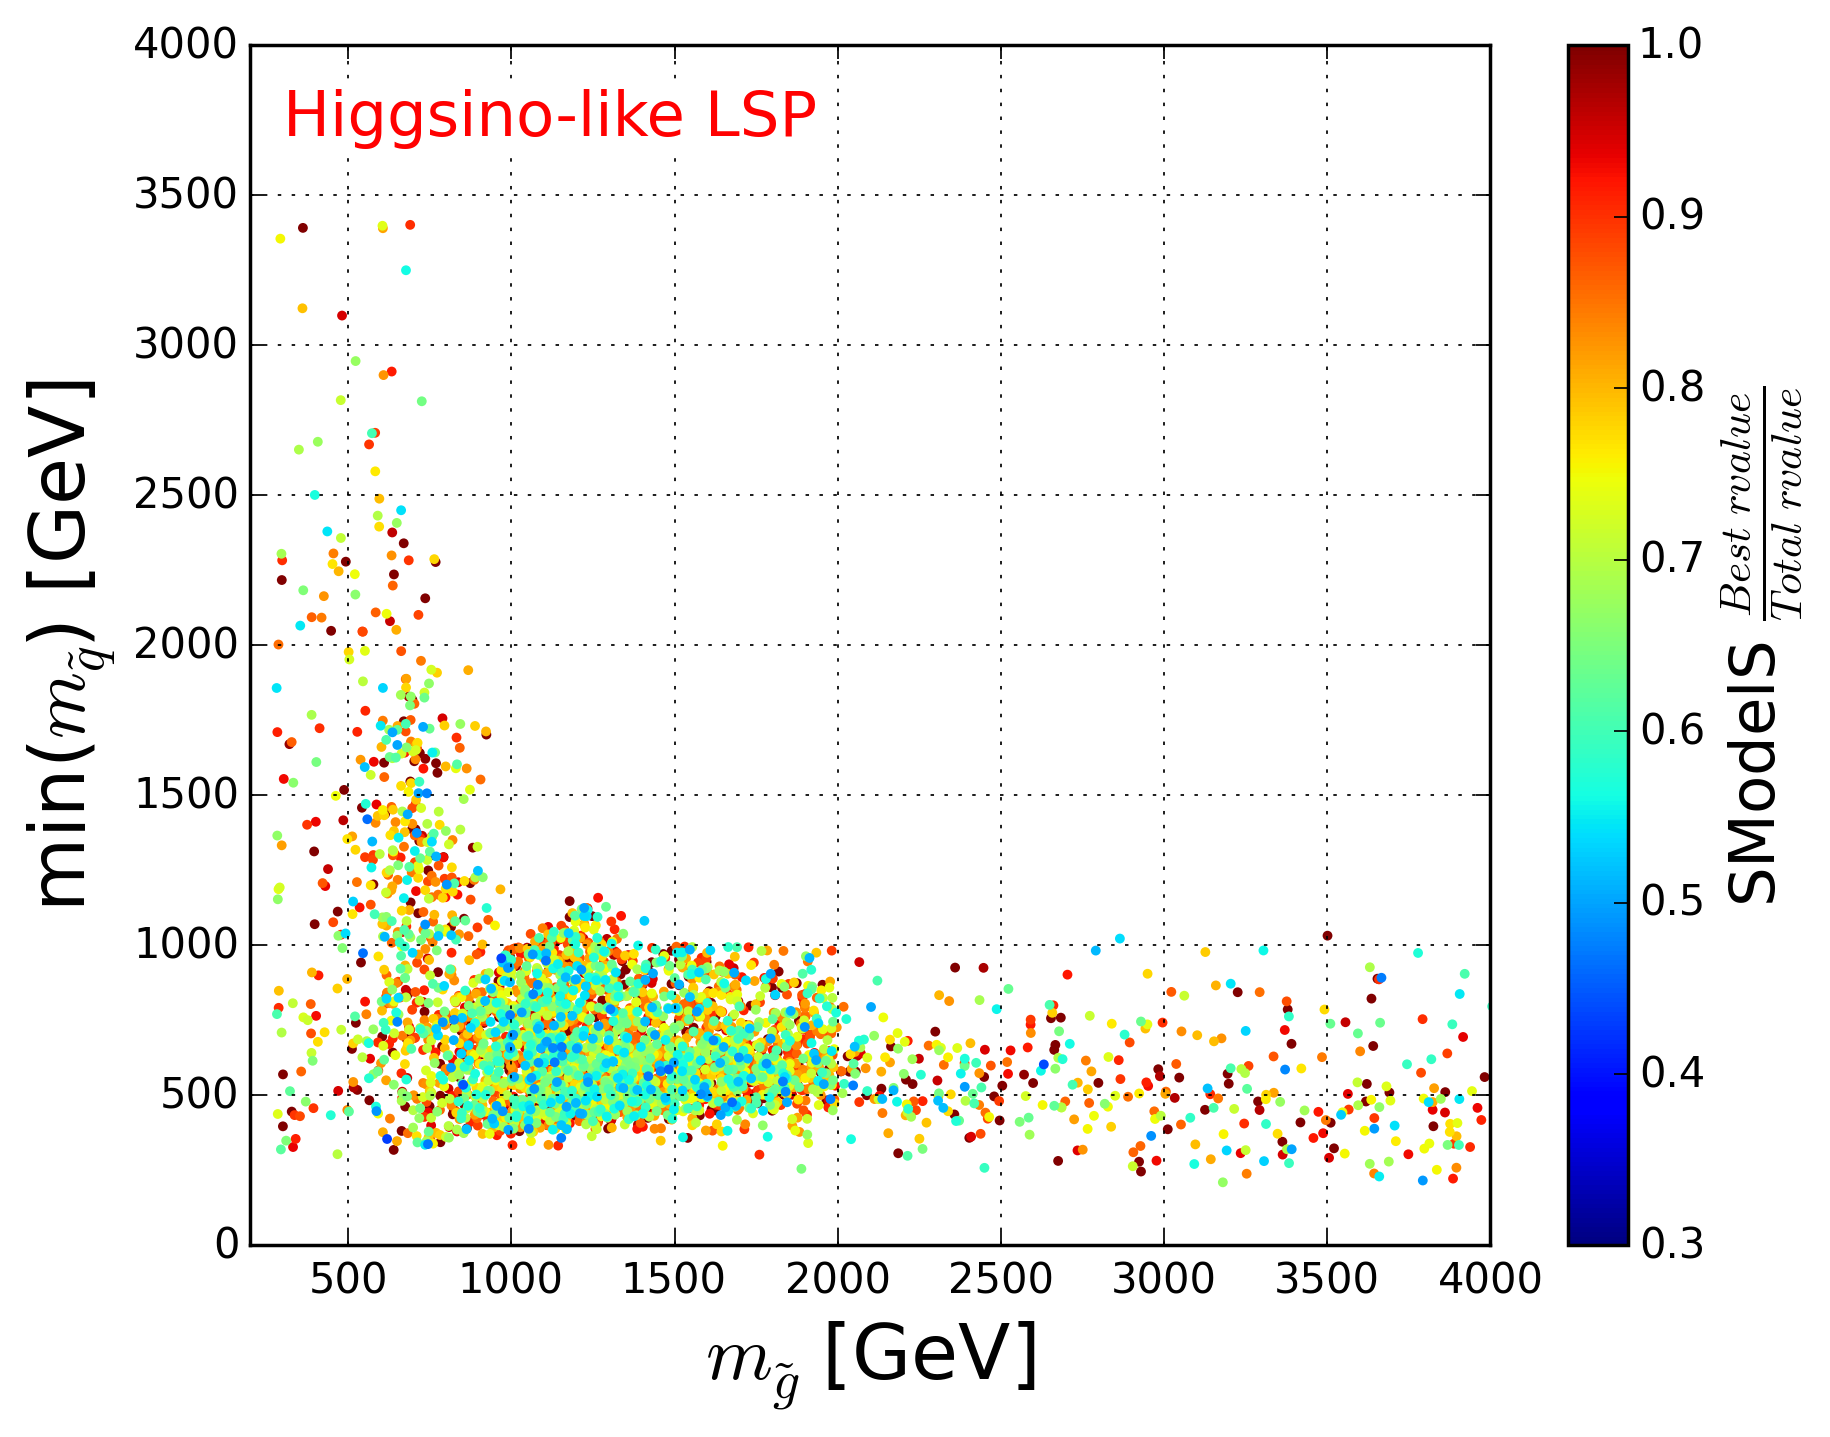
\includegraphics[width=0.49\textwidth]{PLOTS/Weights/HIGGSINO_rValus_Glu_Sq_Ratio.png}}
\end{center}
\caption{Fractional contribution of the model with the highest rvalue to the total rvalue. Points in dark blue benefit from the combination of the three results for \textit{T2}, \textit{T5} and \textit{T3GQ}.} 
\label{rValues}
\end{figure}
%
Finally, in Fig.\ref{Histos_r}, the distributions of the rvalues for each result of the analysis ATLAS-SUSY-2013-02 (\textit{T1},\textit{T2},\textit{T5} and \textit{T3GQ}), the combinations of models (\textit{T2+T5}, \textit{T2+T5+T3GQ} and the sum of all the available results \textit{T1+T2+T5+T3GQ}) is show. Only the points excluded by the analysis are considered; this implies that the points in the first bin $0\leq r < 1$ can be excluded only by considering the sum of all the results, i.e. considering \textit{T1+T2+T5+T3GQ}. For the bins with $r \geq 1$, each individual contribution might be sufficient to exclude the models tested. For large rvalues, the number of points decreases as expected, and the importance of the combinations of multiple results increases. The last bin refers to $rvalue \geq 10$, i.e. points that can be strongly excluded by the SMS results considered, in particular by the combination of the \textit{T1+T2+T5+T3GQ} and \textit{T2+T5+T3GQ} for the Bino and Higgsino-like LSP case respectively. 
\begin{figure}[!]
\begin{center}
\subfigure
{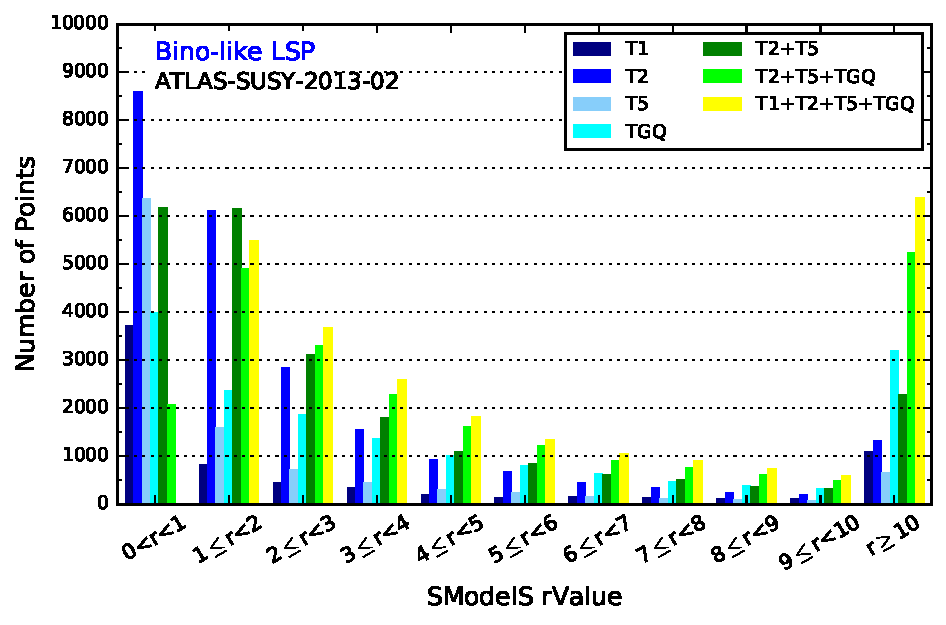
\includegraphics[width=0.49\textwidth]{PLOTS/Combination/ATLAS-SUSY-2013-02_Bino_rValuesHisto.pdf}}
\subfigure
{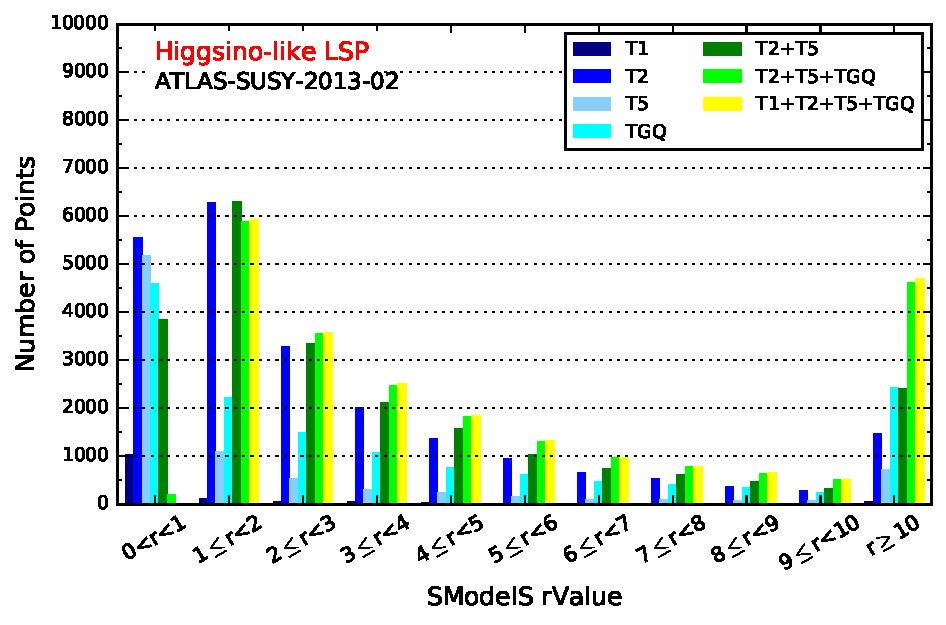
\includegraphics[width=0.49\textwidth]{PLOTS/Combination/ATLAS-SUSY-2013-02_Higgsino_rValuesHisto.pdf}}
\end{center}
\caption{Distribution of the rvalues for excluded points, considering single SMS or combinations, for the analysis ATLAS-SUSY-2013-02.} 
\label{Histos_r}
\end{figure}

%
%\begin{figure*}
%\begin{center}
%\subfigure
%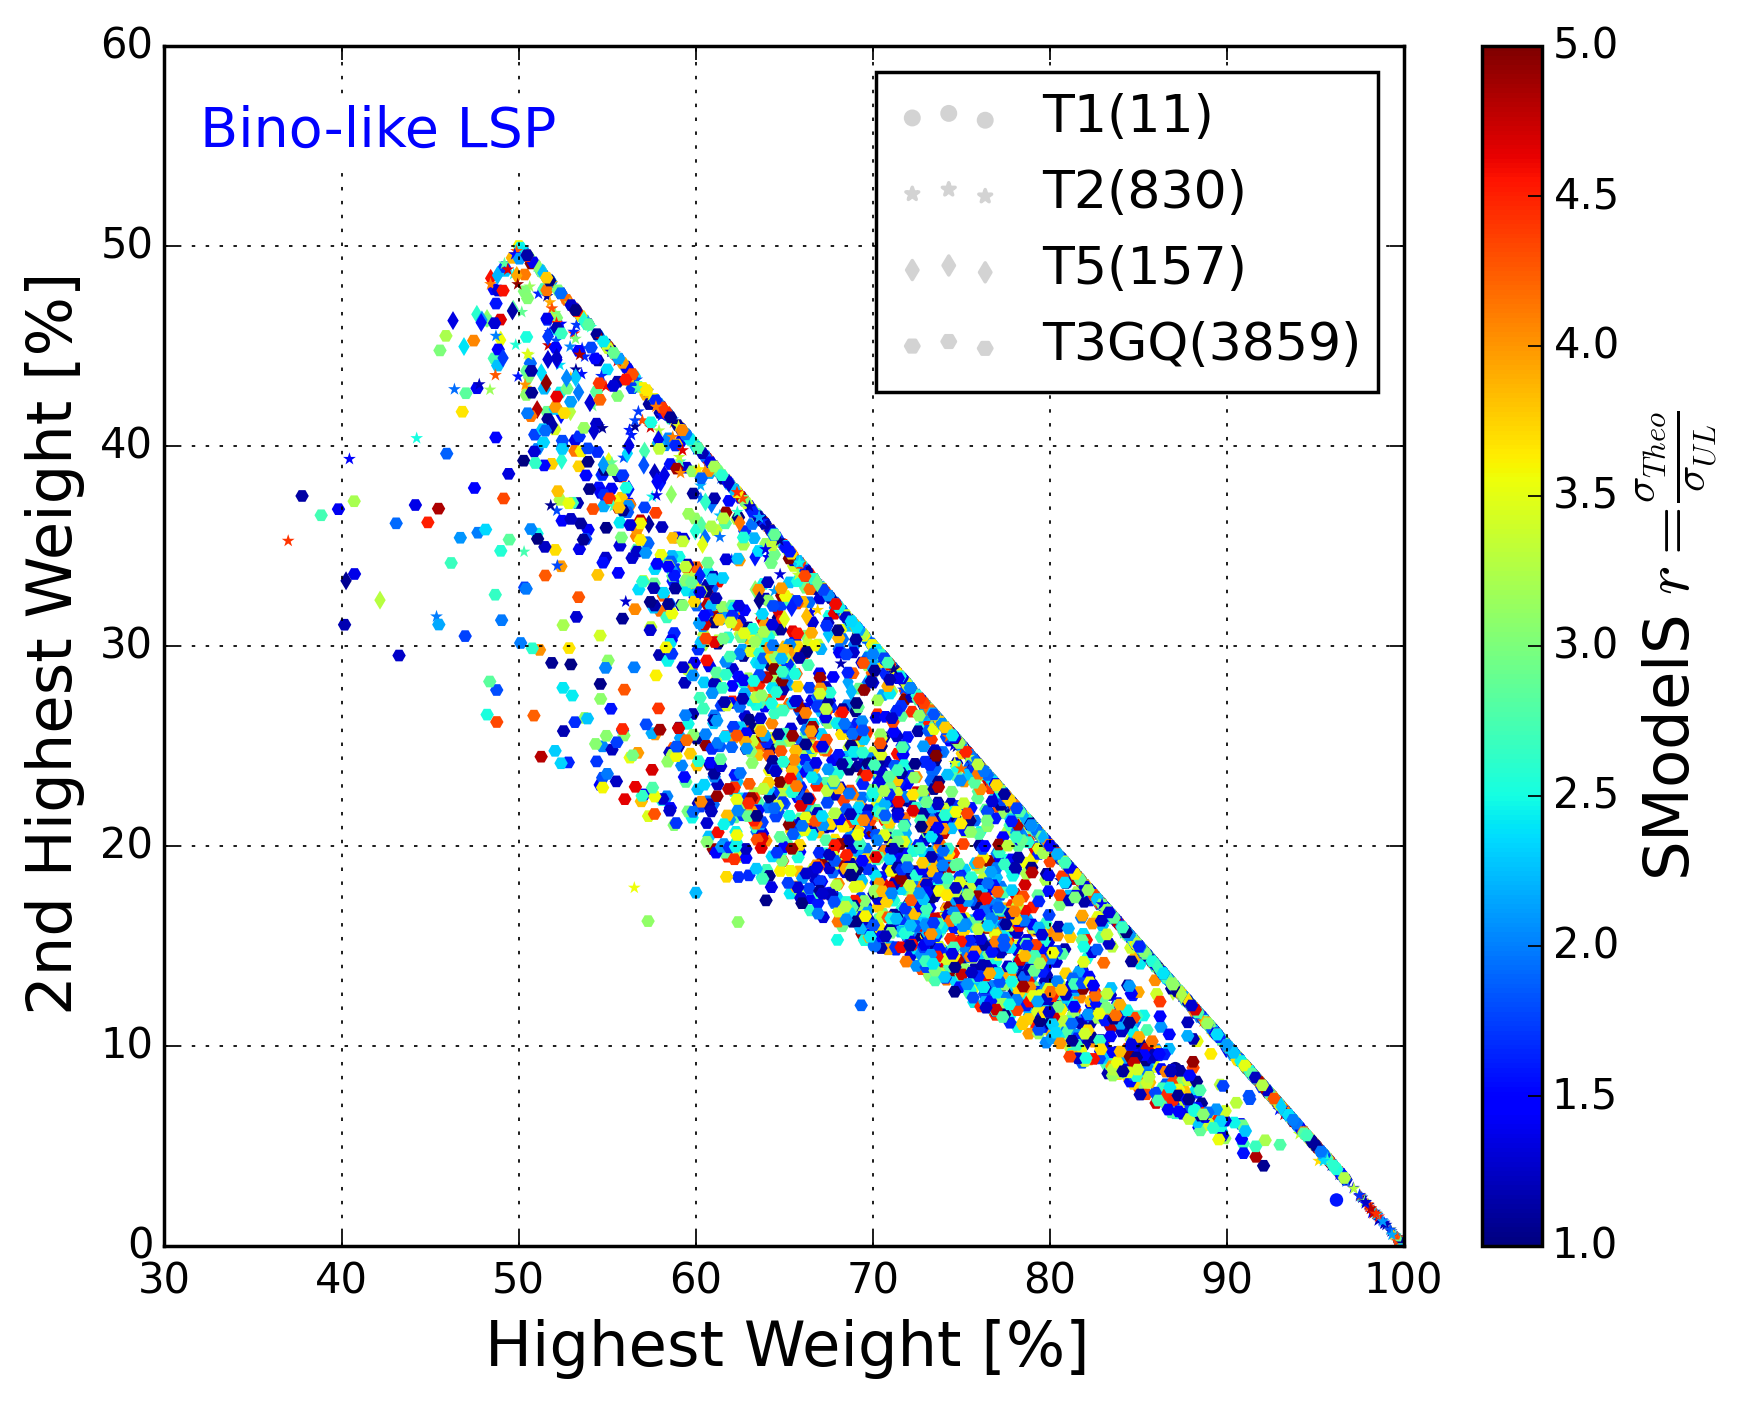
\includegraphics[width=0.49\textwidth]{PLOTS/Weights/Weight_Fraction_r5BINO.png}
%\subfigure
%{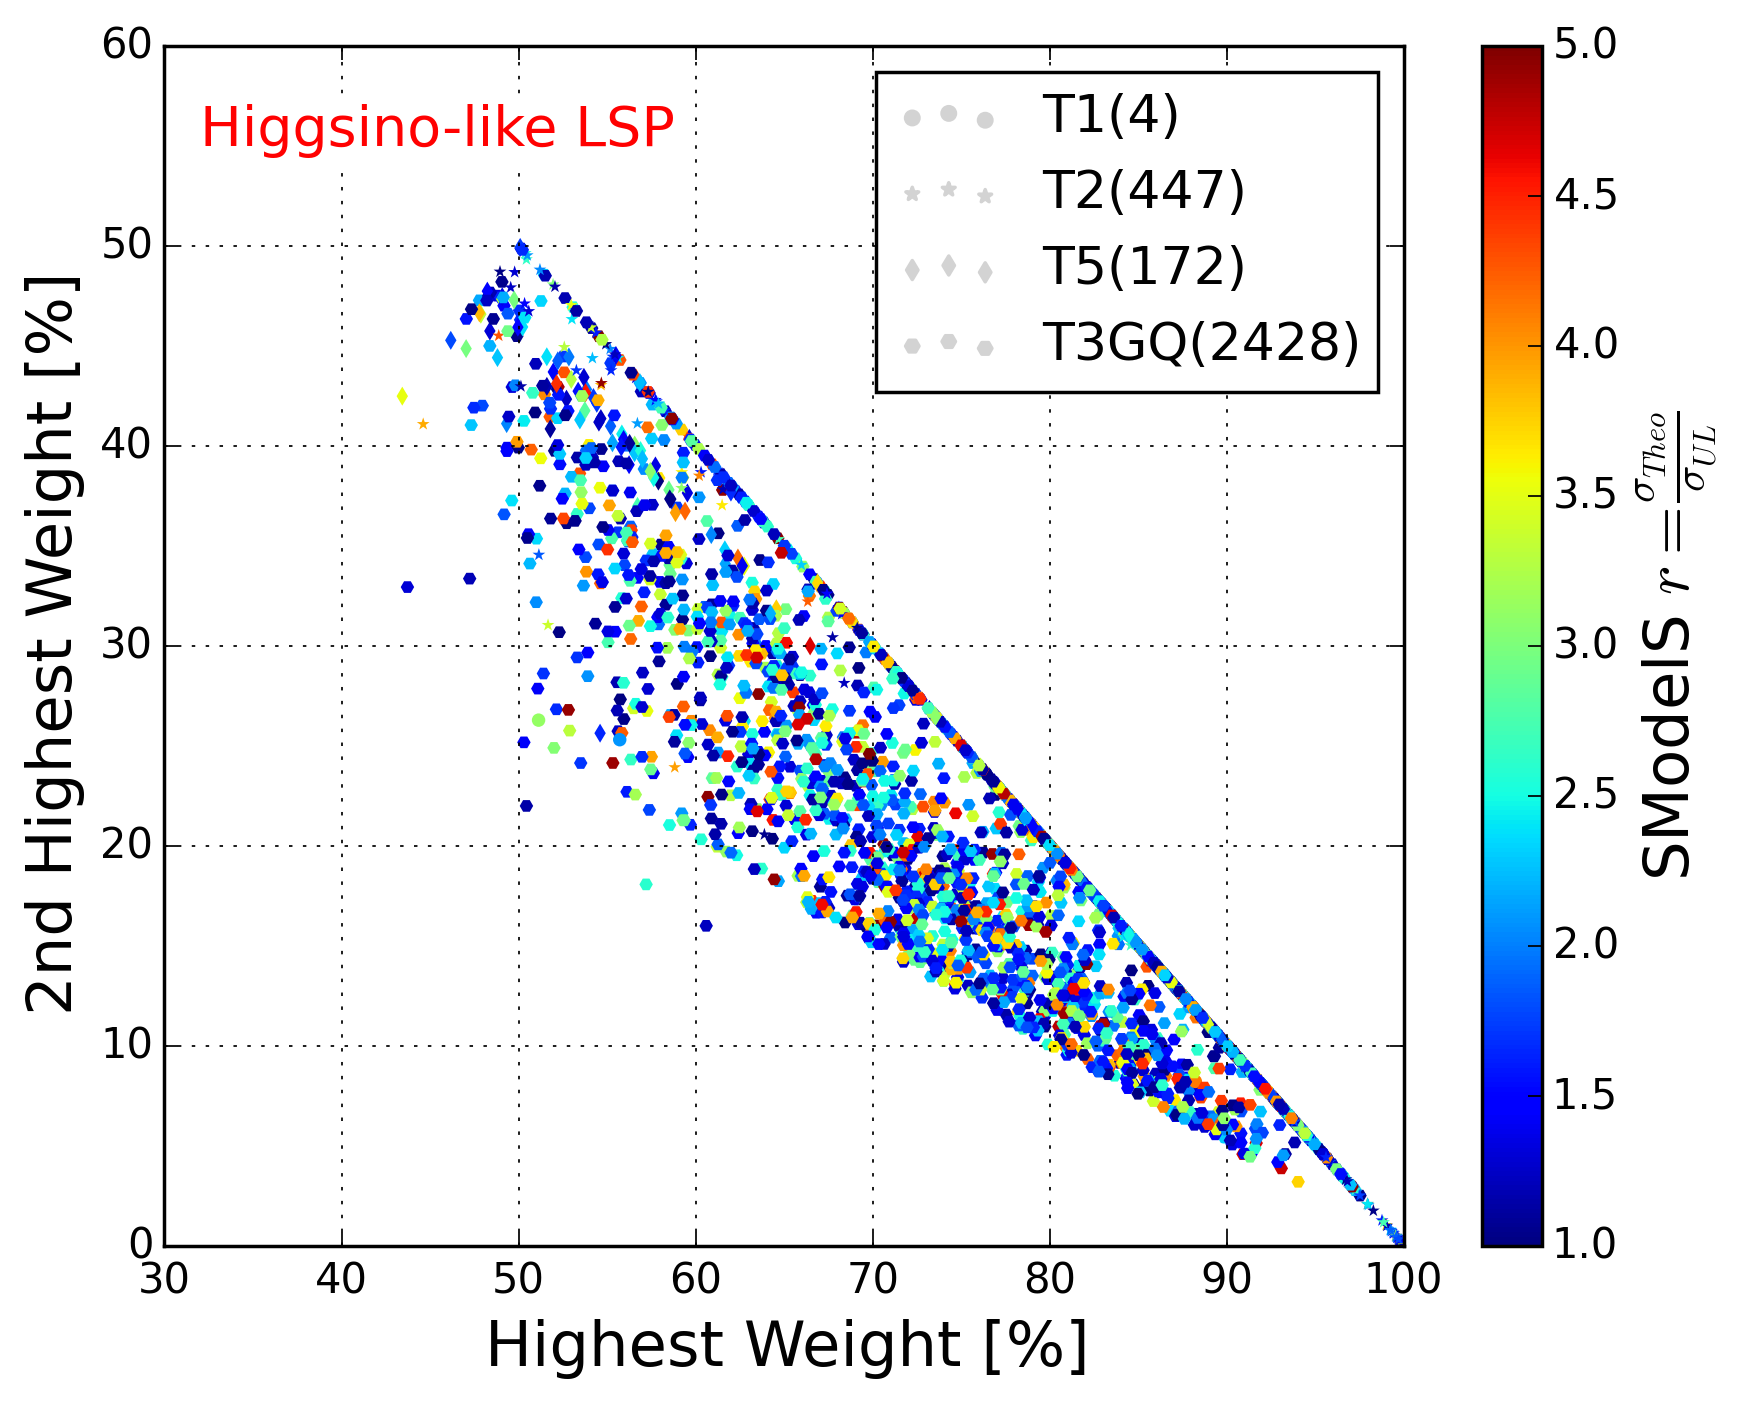
\includegraphics[width=0.49\textwidth]{PLOTS/Weights/Weight_Fraction_r5HIGGSINO.png}}
%\end{center}
%\caption{$\%$ contribution to the total weight of the highest (x-axis) and second highest (y-axis) topology, for the Bino-like (left) and Higgsino-like LSP (right). The topology leading the largest contribution is indicated with different marks. The color maps report the total rvalue for the analysis ATLAS-SUSY-2013-02; only points with rvalue<5 are shown. 
%{\color{blue} add ATLAS-02 label} }
%\label{rValues}
%\end{figure*}
%
%\subsection{Missing Topologies}
%Finally, it is interesting to have a look at the most important missing topologies. 
%\begin{figure}[!]
%\begin{center}
%\subfigure
%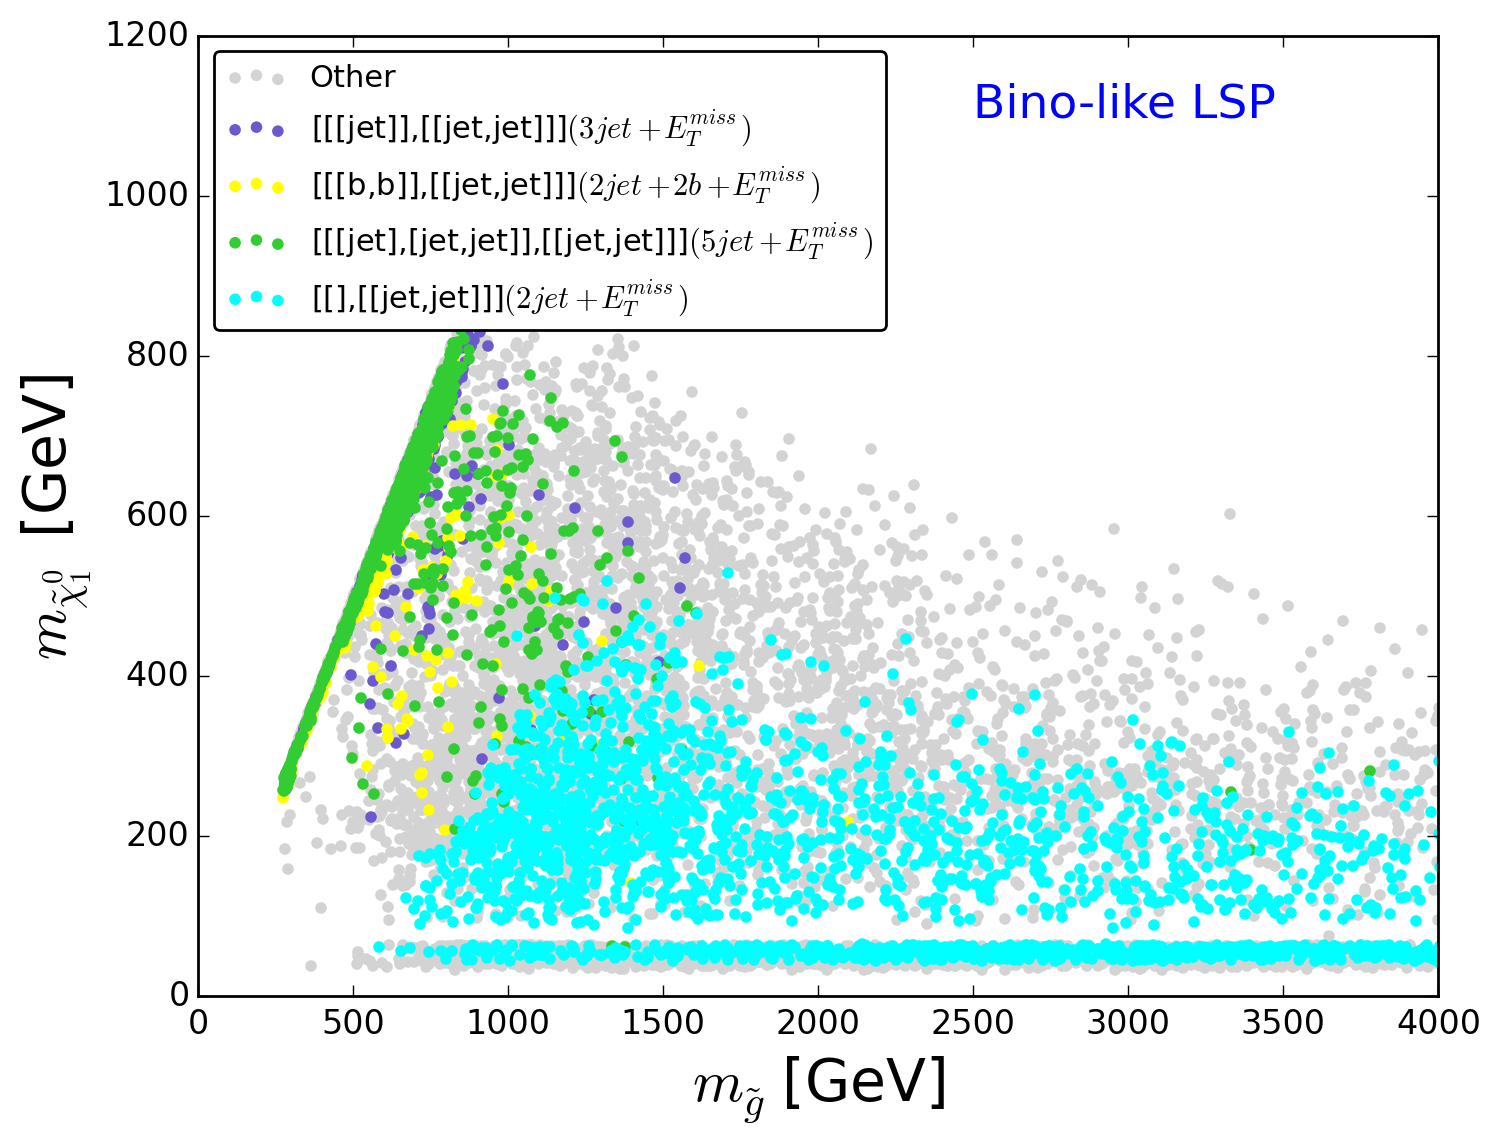
\includegraphics[width=0.49\textwidth]{PLOTS/Missing/BINO_Missing_GluNeu.png}
%\subfigure
%{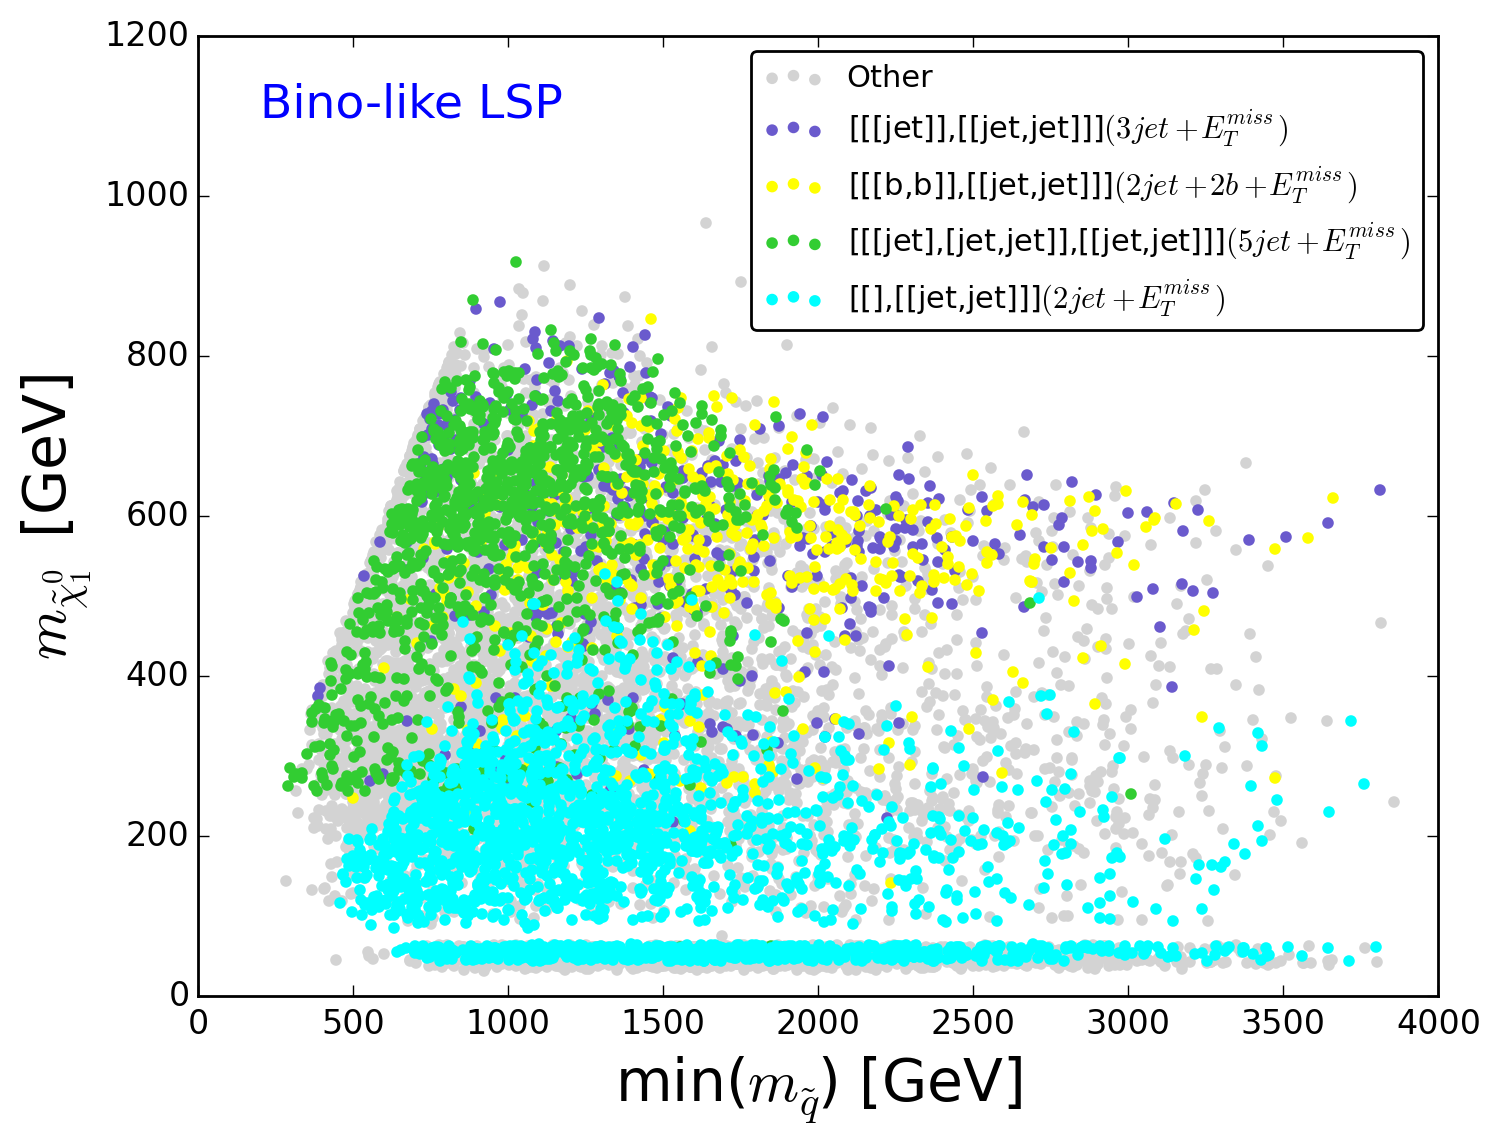
\includegraphics[width=0.49\textwidth]{PLOTS/Missing/BINO_Missing_SqNeu.png}}
%\subfigure
%{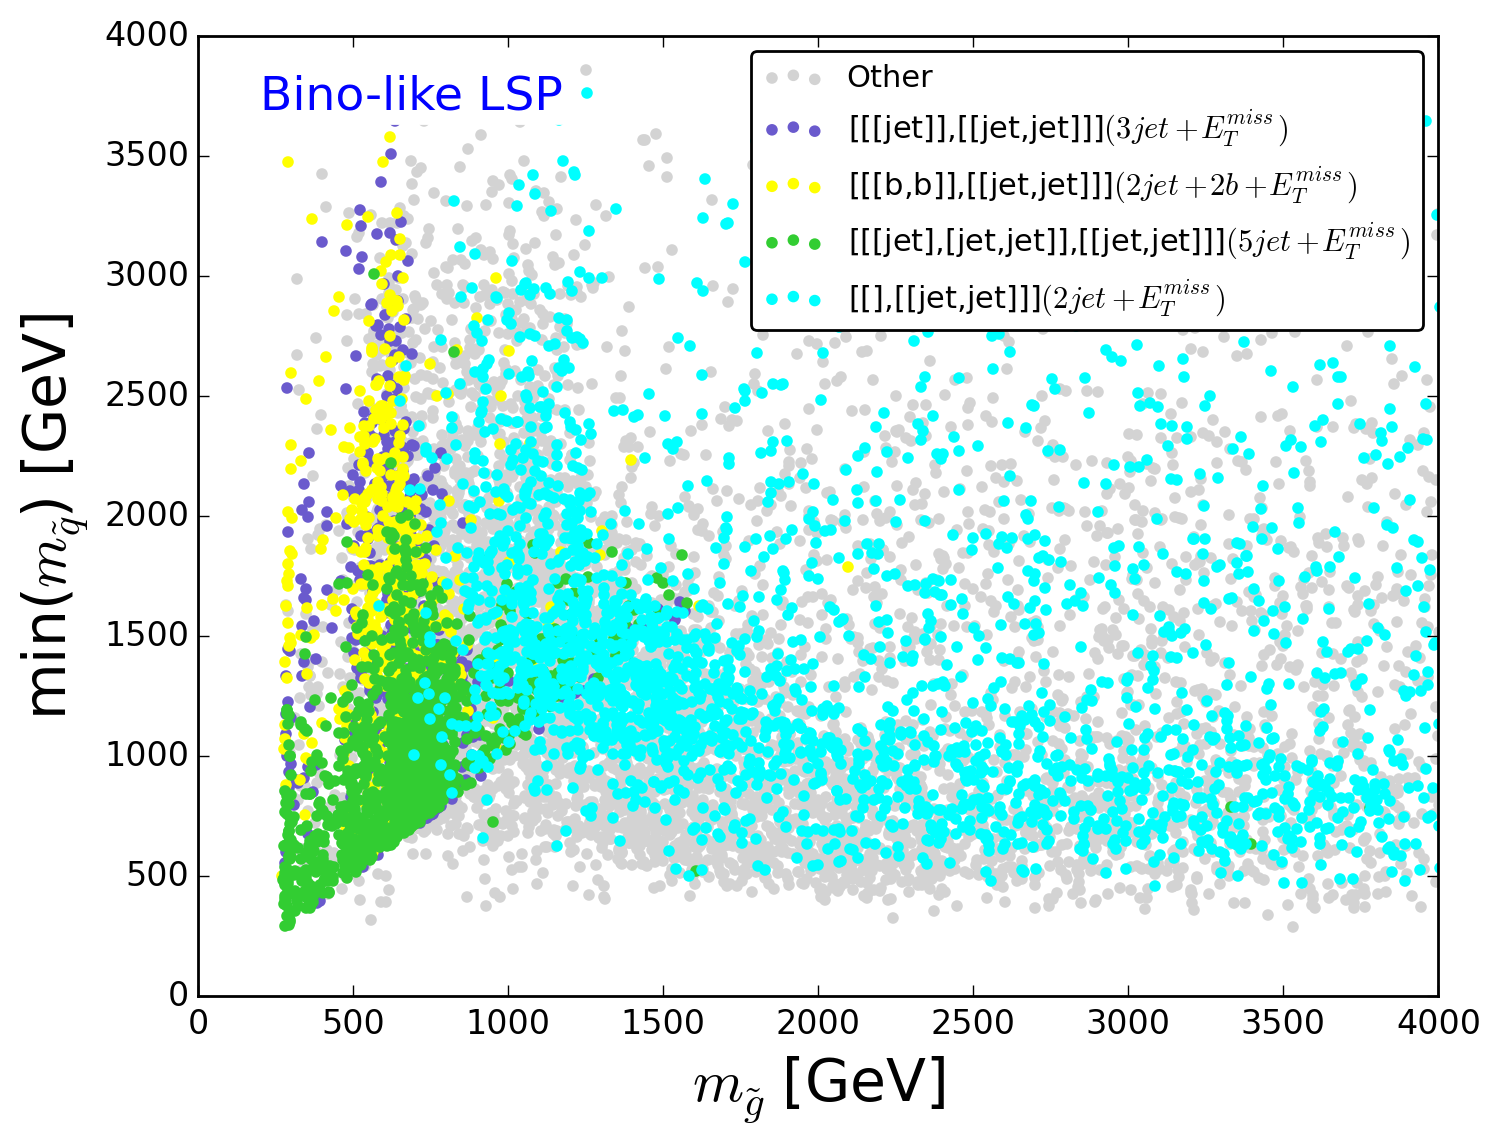
\includegraphics[width=0.49\textwidth]{PLOTS/Missing/BINO_Missing_GluSq.png}}
%\subfigure
%{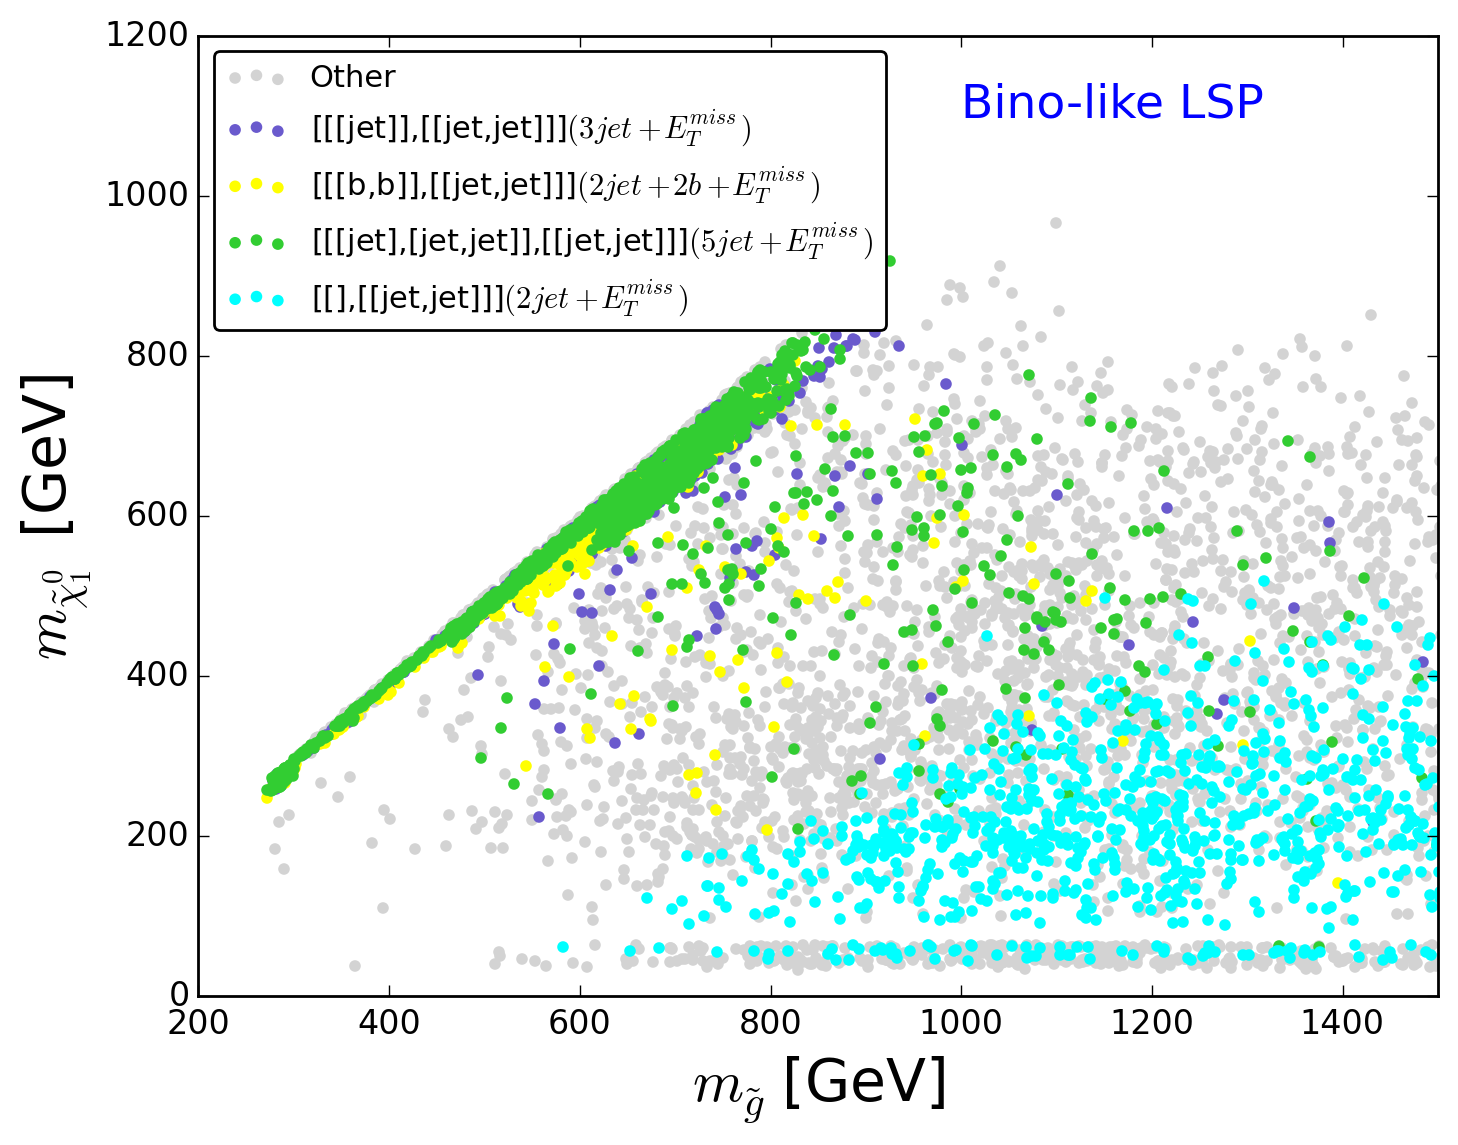
\includegraphics[width=0.49\textwidth]{PLOTS/Missing/BINO_Zoom_Missing_GluNeu.png}}
%\end{center}
%\caption{Missing topologies with the highest weights for the Bino-like LSP dataset.} 
%\label{Missing_Bino}
%\end{figure}
%
%\begin{figure}[!]
%\begin{center}
%\subfigure
%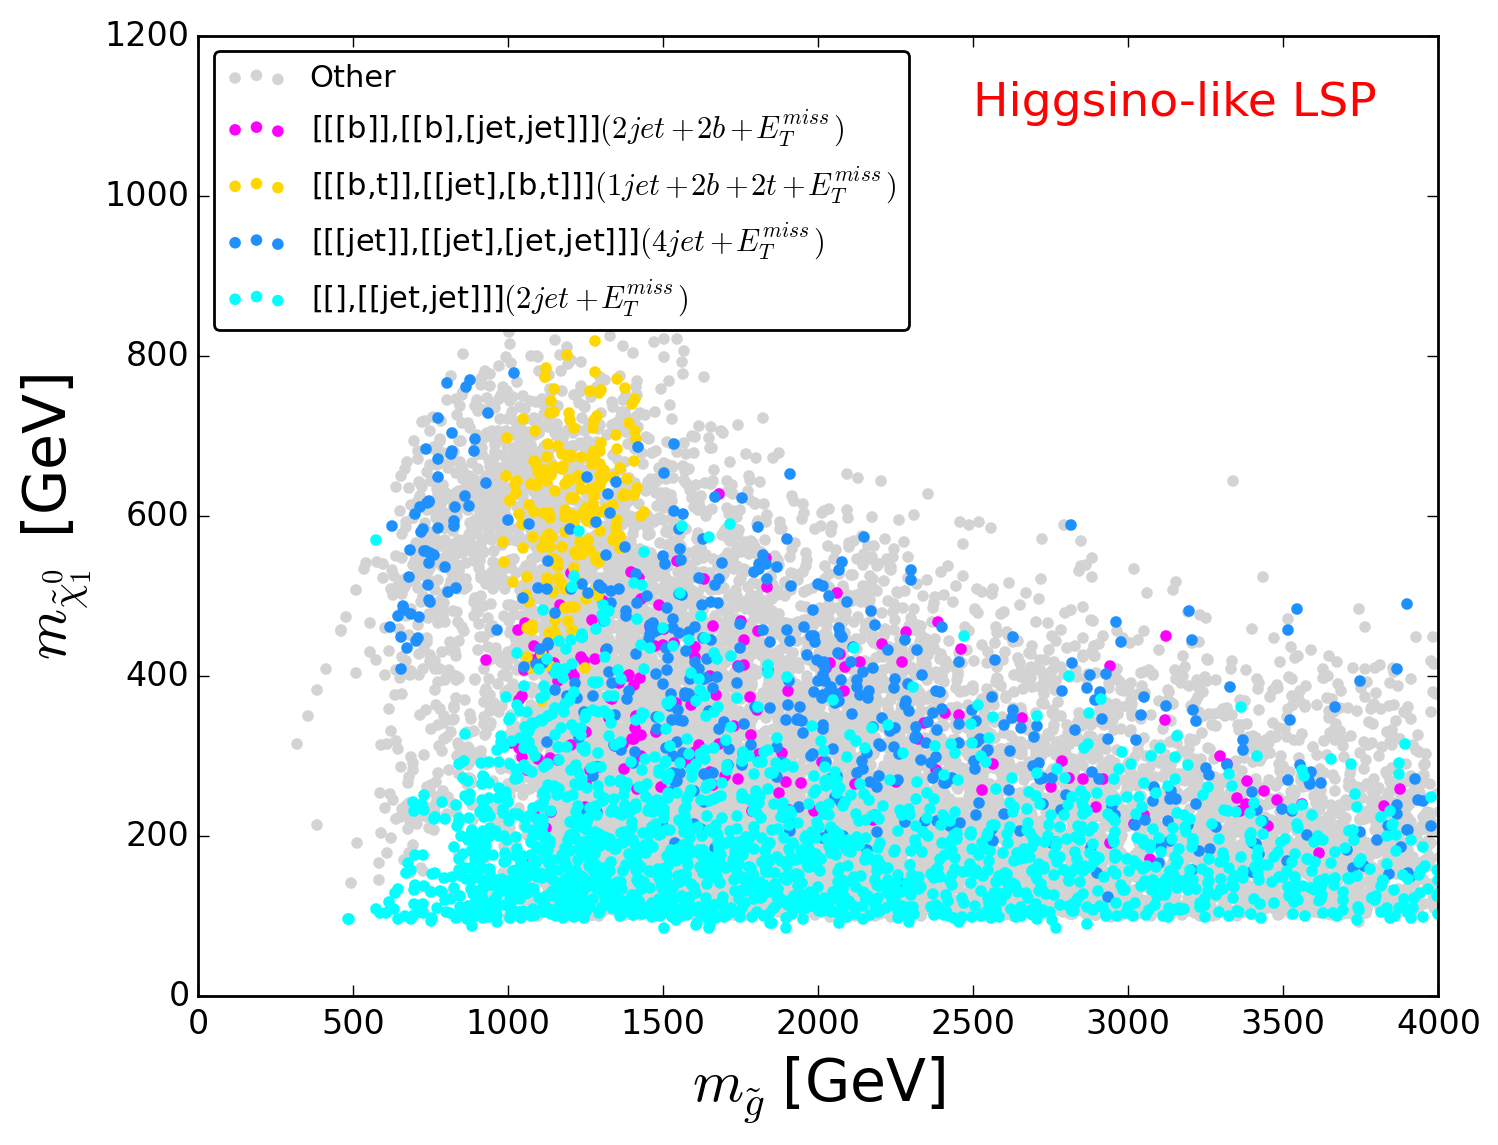
\includegraphics[width=0.49\textwidth]{PLOTS/Missing/HIGGSINO_Missing_GluNeu.png}
%\subfigure
%{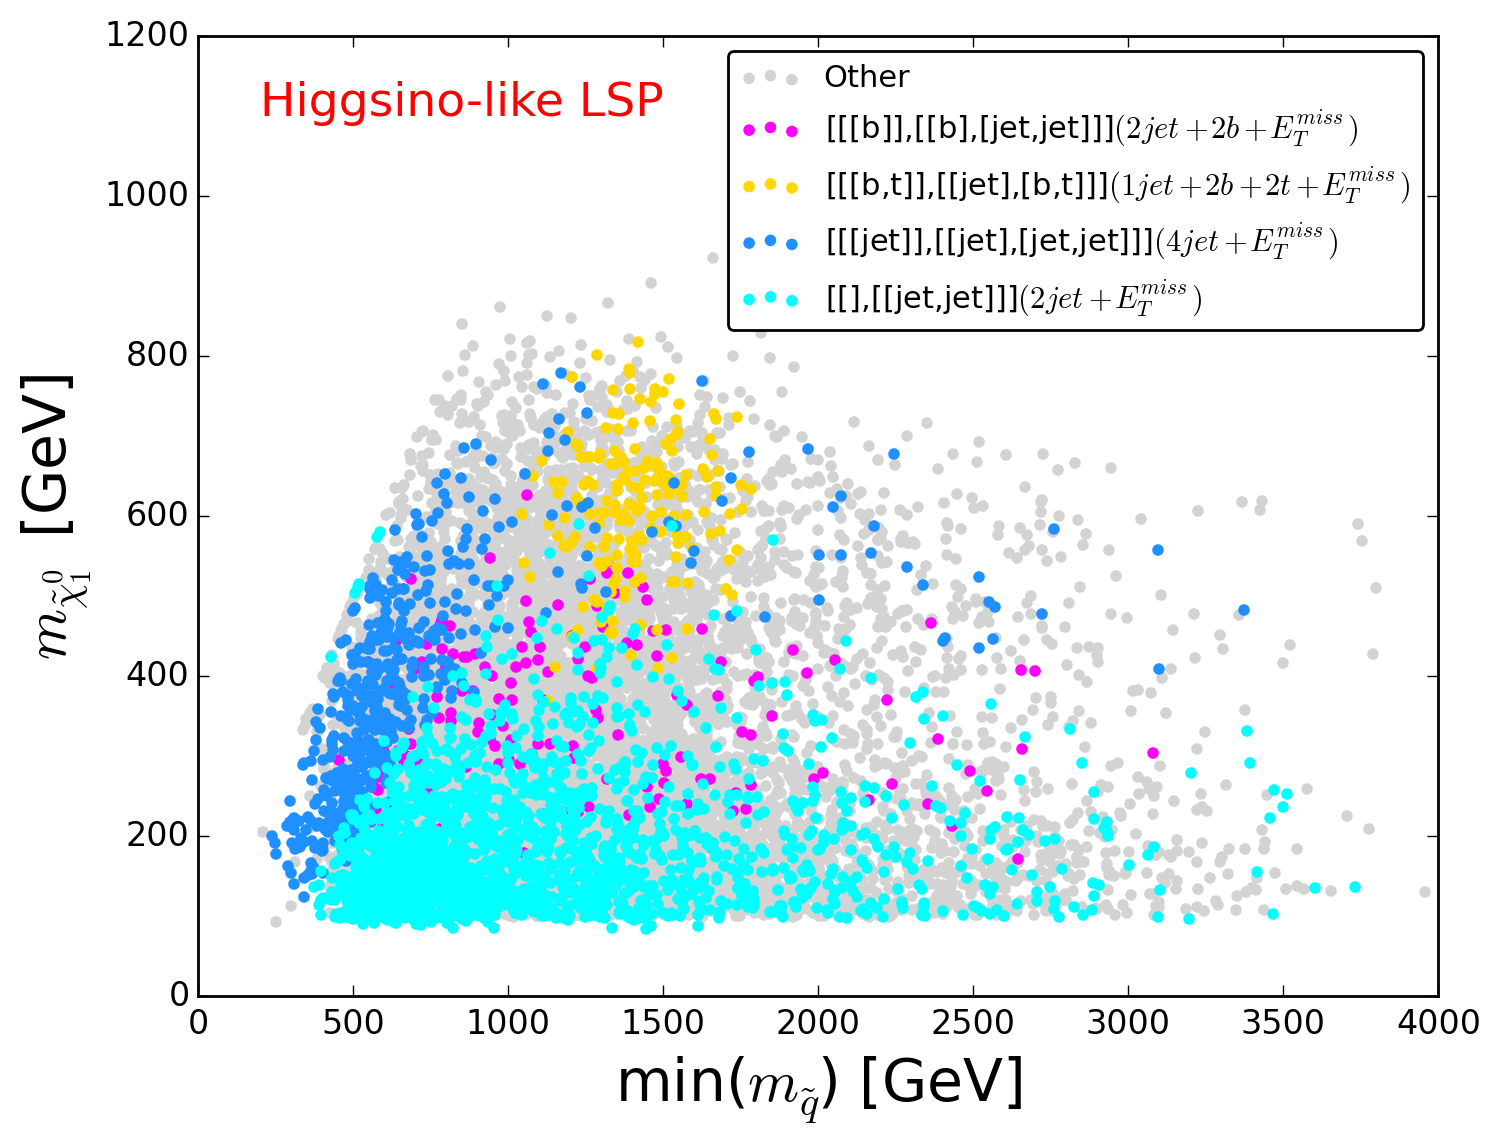
\includegraphics[width=0.49\textwidth]{PLOTS/Missing/HIGGSINO_Missing_SqNeu.png}}
%\subfigure
%{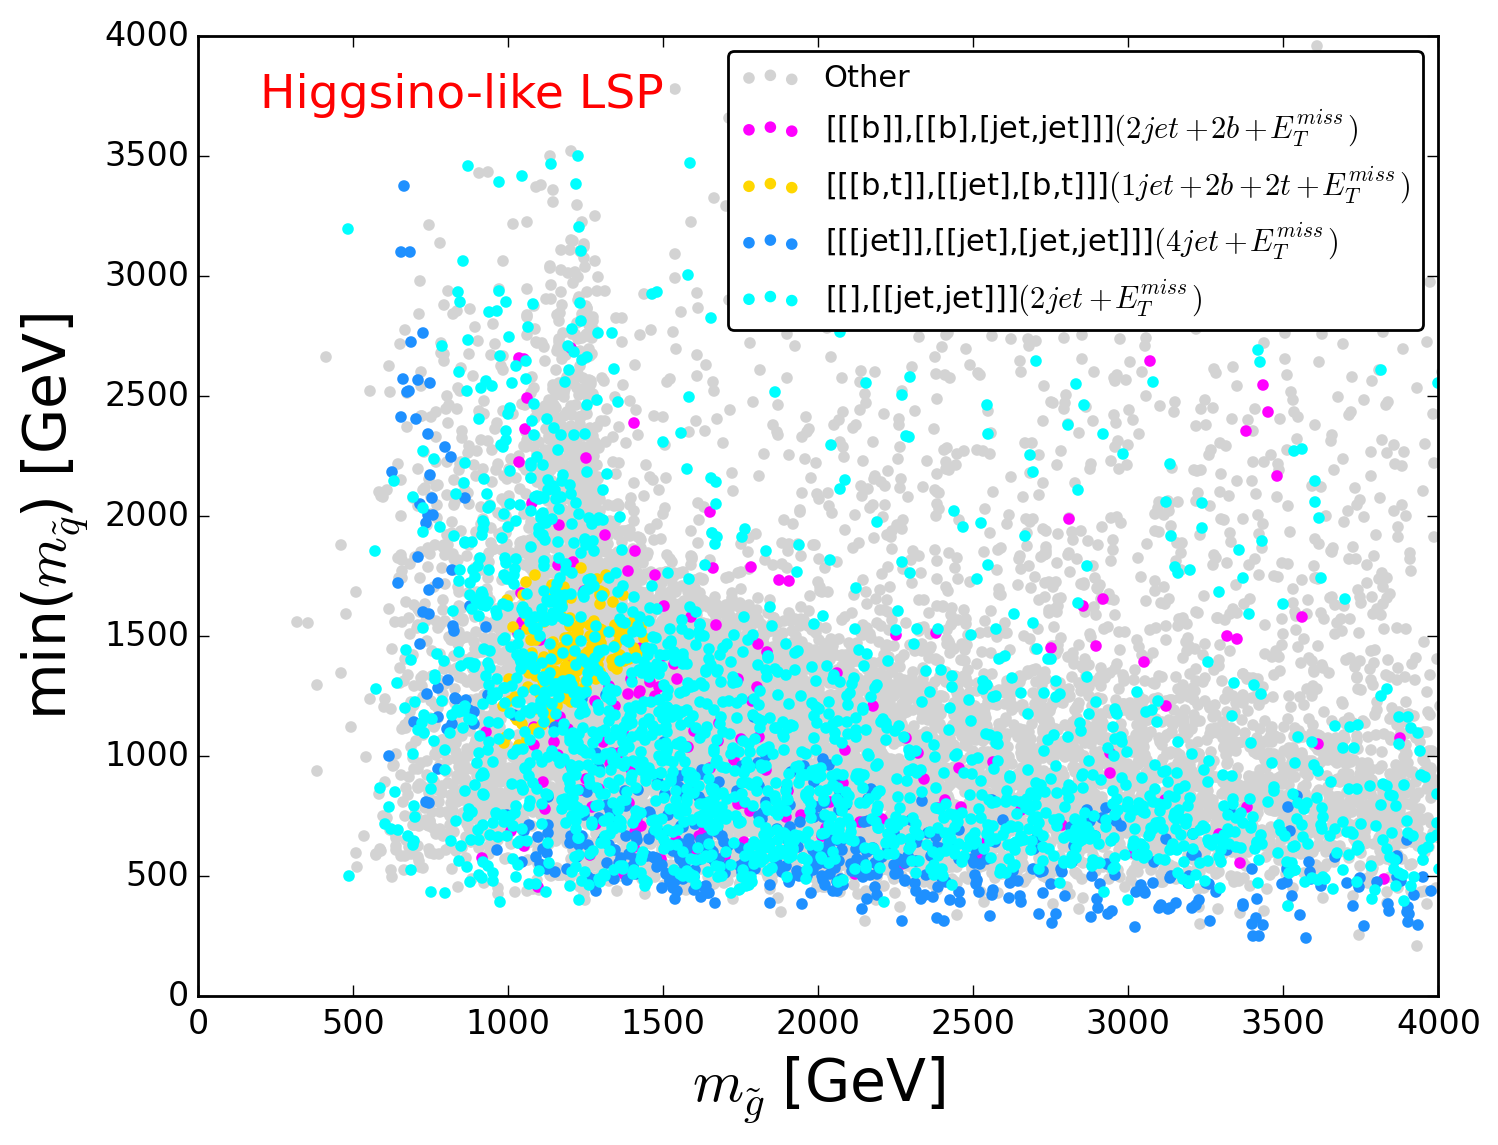
\includegraphics[width=0.49\textwidth]{PLOTS/Missing/HIGGSINO_Missing_GluSq.png}}
%\subfigure
%{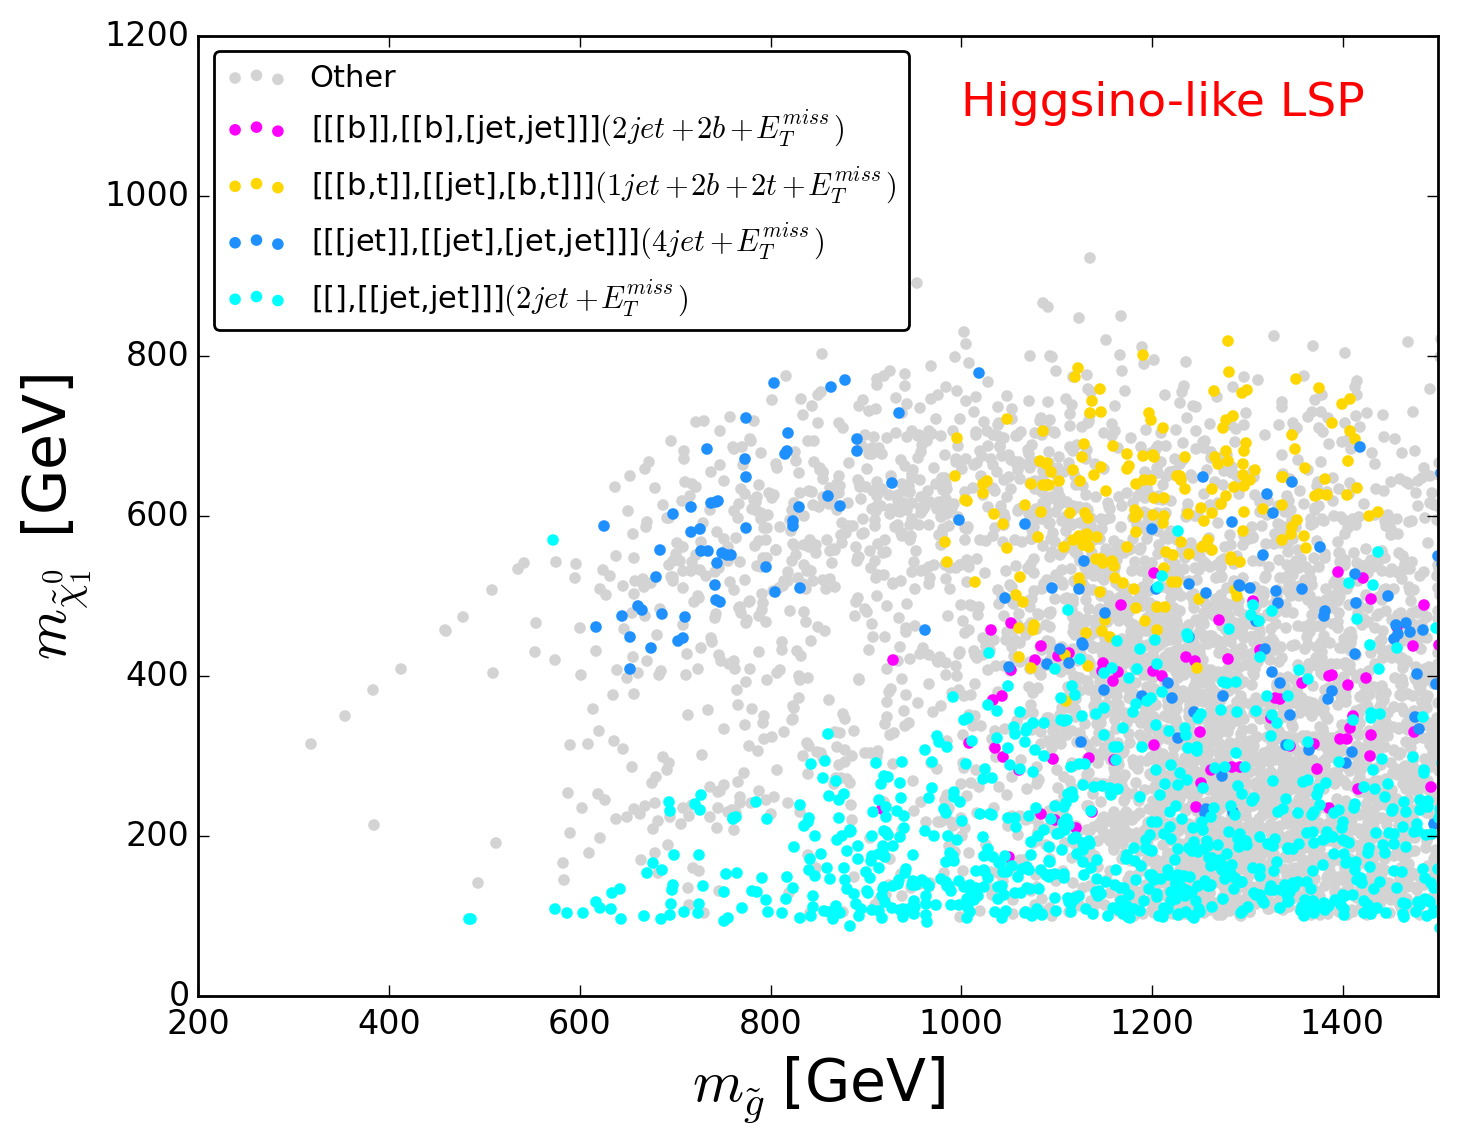
\includegraphics[width=0.49\textwidth]{PLOTS/Missing/HIGGSINO_Zoom_Missing_GluNeu.png}}
%\end{center}
%\caption{Missing topologies with the highest weights for the Higgsino-like LSP dataset.} 
%\label{Missing_Higgsino}
%\end{figure}
%


%\section{Comparison with 13 TeV Results}
%
%In general it is believed that the latest results from the LHC experiments, obtained with data collected at 13 TeV centre-of-mass energy, provide better limits with respect the analogous results obtained by previous 8 TeV searches. Besides an improvmeent in the collision energy, recent searches are also based on larger dataset, due to a large integrated luminosity wrt Run 1. In the context of simplified models, however, such belief is not totally justified, depending primarily on the type of simplified model that are used for the interpretation of the searches. Besides few results provided by the ATLAS collaboration, see e.g. {\color{blue} to do}, in the form of efificnecy maps, only upper limit results are available, relative to limited variety of simplified models. It is interesting then to investigate if there are pMSSM points that can be excluded at 8 TeV thanks to the \TGQ~homegrown results, but that survive 13 TeV constraints with the available simplified models. Table \ref{13_TeV} summarises the number of points that cannot be excluded with 13 TeV results. 
%
%\begin{table*}
%\center
%\renewcommand{\arraystretch}{1.3}
%\begin{tabular}{ l | c   c  }
%\textbf{Number of Points} & \textbf{Bino-like LSP }& \textbf{Higgsino-like LSP} \\
%\toprule \toprule
%Non Decoposed  & 256 & \\
%Non Excluded & 262  &  { \color{blue} xxx } \\
%Total Non Constrained  & 518 & \\
%\\ 
%\hline
%\end{tabular}
%\caption{Summary of points excluded by the newdly added 8 TeV EMs results, that cannot be escluded at 13 TeV (see text for details about the 13 TeV results considered.} }
%\label{13_TeV}
%\end{table*}

%{\color{blue} Ideally, make a cmparison with the T2 results *only*} 





\section{Conclusion}
Despite a plethora of available simplified model results, in the form of upper limit or efficiency maps, a large portion of the parameter space of a full theory like the pMSSM cannot be properly constrained. This is well known in the case of model points with complicated mass spectra originating long decay patterns, which are hardly constrained also by means of full recast procedures. Fortunately, there exist a number of simplified models involving only three SUSY particles and sort decay chains that captures a large fraction of the signals from gluino-squark associated production. Thanks to the available recasting tools, it is possible to cover these important addtional signatures by re-interpreting existing ATLAS and CMS searches and produce dedicated EM results. This work constitutes the first example, and proof-of-concept, that tools such as \SMO~ can be used to extend the available results, those being provided by the LHC collaborations or produced by group of phenomenologists, to cover region of the parameter space not previously investigated by SMS. Using EM results has the advantage of allowing the combination of multiple signals. This is necessary for the exclusion of certain models, for which either many production channels or many possible decay chains for the same channel are available. The importance of the latter was already pointed out in \cite{Ambrogi:2017lov} for the decays of third generatin squarks via intermediate gauginos, for which the number of available simplified model results is limited. 
The former was extensively discussed in this work for sufficiently light gluinos and squarks so that gluino par production, squark pair production and gluino-squark associated production have sizeable cross sections. 
XXX Quote the number of pointes excluded by ATLAS analysis only



%
\acknowledgments
The author thanks the Institut f\"ur Hochenergiephysik of the \"Osterreichische Akademie der Wissenschaften for the opportunity to use the computing facilities.
%


\clearpage
\appendix
\ONE
\section{T3GQ vs T3QG Upper Limits}
The following Tables \ref{ATLAS02_UL} and \ref{ATLAS02_UL_2}  compare the upper limits obtained for the mass point ($M_1,M_2,M_3) = (1000,200,190),(1200,600,500)$ [GeV] for the two different hierarchy models \textit{T3GQ}($m_{\tilde g}, m_{\tilde q}, m_{\tilde \chi _1 ^0 }$) and \textit{T3QG}($m_{\tilde q}, m_{\tilde g}, m_{\tilde \chi _1 ^0 }$). In bold, the best SR providing the strongest expected limit and corresponding observed limit is shown. The difference in the efficiency and consequent choice of a different SR, respectively \textit{2jm} for \textit{T3GQ} and \textit{2jt} for \textit{T3QG}, favours a strongest limit for the \textit{T3GQ} case. However the difference is contained within a factor 2, which translates to only few tens of GeV difference in the excluded mass of Squarks or Gluinos. The value of the observed UL, quoted by \SMO, is indicated with an asterisk. 

\begin{table*}[h]
\centering
\renewcommand\arraystretch{1.3} 
\scriptsize
\begin{tabular}{ l c c    c c c  |  c c c  }
\toprule \toprule
\multicolumn{3}{c}{($M_1,M_2,M_3) = (1000,200,190)$} & \multicolumn{3}{c}{ \textbf{T3GQ}} & \multicolumn{3}{c}{ \textbf{T3QG}} \\  \toprule 
\textbf{SR} & $UL_{exp}$ & $UL_{obs}$ & $\epsilon$ &  $UL_{exp}/\epsilon$ & $UL_{obs}/\epsilon$ & $\epsilon$ & $UL_{exp}/ \epsilon$ & $UL_{obs}/ \epsilon$ \\
2jm & 5.552 &  4.242 &  0.118  & \textbf{47.1} &  \textbf{36.0}  &  0.090 &  \textbf{61.5}*  & \textbf{47.0}*\\
2jt  & 1.512  & 1.818 &  0.032  & \textbf{47.9} &  \textbf{57.5}  &  0.027 &  \textbf{56.1}  & \textbf{67.4} \\
3j &  0.332 &  0.433  & 0.002 &  139.4 &  182.2  &  0.002 &  186.4 &  243.6 \\ 
4jl  & 5.435 &  4.749  & 0.032  & 171.4  & 149.8  &  0.039 &  139.7  & 122.1 \\
4jl-  & 11.561 &  13.292 &  0.036  & 318.7 &  366.4  &  0.047 &  248.0 &  285.2 \\
4jt  & 0.240  & 0.149  & 0.002  & 146.1  & 90.8 &   0.001  & 178.1  & 110.8 \\
5j  & 1.714  & 1.543  & 0.007 &  245.1 &  220.7  &  0.010  & 172.9  & 155.6 \\
6jl  & 1.531  & 1.923  & 0.002  & 965.5 &  1212.5  & 0.003  & 555.5 &  697.7 \\
6jt &  0.333  & 0.332 &  0.001  & 472.8  & 470.4 &  0.001 &  327.8  & 326.2 \\
6jt+  & 0.302 &  0.399 &  0.001  & 428.6  & 566.3  & 0.001  & 297.2  & 392.7 \\
\bottomrule \bottomrule
\end{tabular}
\caption{Summary of the UL for the SRs of ATLAS-SUSY-2013-02, for the \textit{T3GQ} and \textit{T3QG} models, with mass spectrum ($M_1,M_2,M_3) = (1000,200,190)$ [GeV] . In bold, the expected and observed limits for the best SRs are highlited. With a star, the value of the observed UL used by \SMO is indicated.}
\label{ATLAS02_UL}
\end{table*}

\begin{table*}[h]
\centering
\renewcommand\arraystretch{1.3} 
\scriptsize
\begin{tabular}{ l c c    c c c  |  c c c  }
\toprule \toprule
\multicolumn{3}{c}{($M_1,M_2,M_3) = (1200,600,500)$} & \multicolumn{3}{c}{ \textbf{T3GQ}} & \multicolumn{3}{c}{ \textbf{T3QG}} \\  \toprule 
\textbf{SR} & $UL_{exp}$ & $UL_{obs}$ & $\epsilon$ &  $UL_{exp}/\epsilon$ & $UL_{obs}/\epsilon$ & $\epsilon$ & $UL_{exp}/ \epsilon$ & $UL_{obs}/ \epsilon$ \\
2jm & 5.552 &  4.242 &  0.178	 &31.172 &	23.815		 &0.184	 &30.111	 &23.004 \\
2jt  & 1.512  & 1.818 &  0.061& 	\textbf{24.623}	& \textbf{29.601}	& 	0.069	& \textbf{21.949}*& 	\textbf{26.385}* \\
3j &  0.332 &  0.433  & 0.005& 	61.421& 	80.255		& 0.005	& 64.971& 	84.893 \\ 
4jl  & 5.435 &  4.749  & 0.165	& 69.892	& 80.356	& 	0.188	& 61.542& 	70.756  \\
4jl-  & 11.561 &  13.292 &  0.145	& 37.596	& 32.851		& 0.166	& 32.813	& 28.672 \\
4jt  & 0.240  & 0.149  & 0.004& 	54.035	& 33.611		& 0.004	& 54.765& 	34.065  \\
5j  & 1.714  & 1.543  &0.048	& 36.043	& 32.449	& 	0.055	& 31.004	& 27.912  \\
6jl  & 1.531  & 1.923  & 0.016	& 98.361	& 123.530	& 	0.018	& 83.039	& 104.286 \\
6jt &  0.333  & 0.332 &  0.008	& 43.713& 	43.489	& 	0.007	& 45.136	& 44.905  \\
6jt+  & 0.302 &  0.399 & 0.008& 	39.632& 	52.359	& 	0.007	& 40.922	& 54.063 \\
\bottomrule \bottomrule
\end{tabular}
\caption{Summary of the UL for the SRs of ATLAS-SUSY-2013-02, for the \textit{T3GQ} and \textit{T3QG} models, with mass spectrum ($M_1,M_2,M_3) = (1200,600,500)$ [GeV]. In bold, the expected and observed limits for the best SR are highlited.}
\label{ATLAS02_UL_2}
\end{table*}


\section{Combination}
\begin{figure}[!]
\begin{center}
\subfigure
{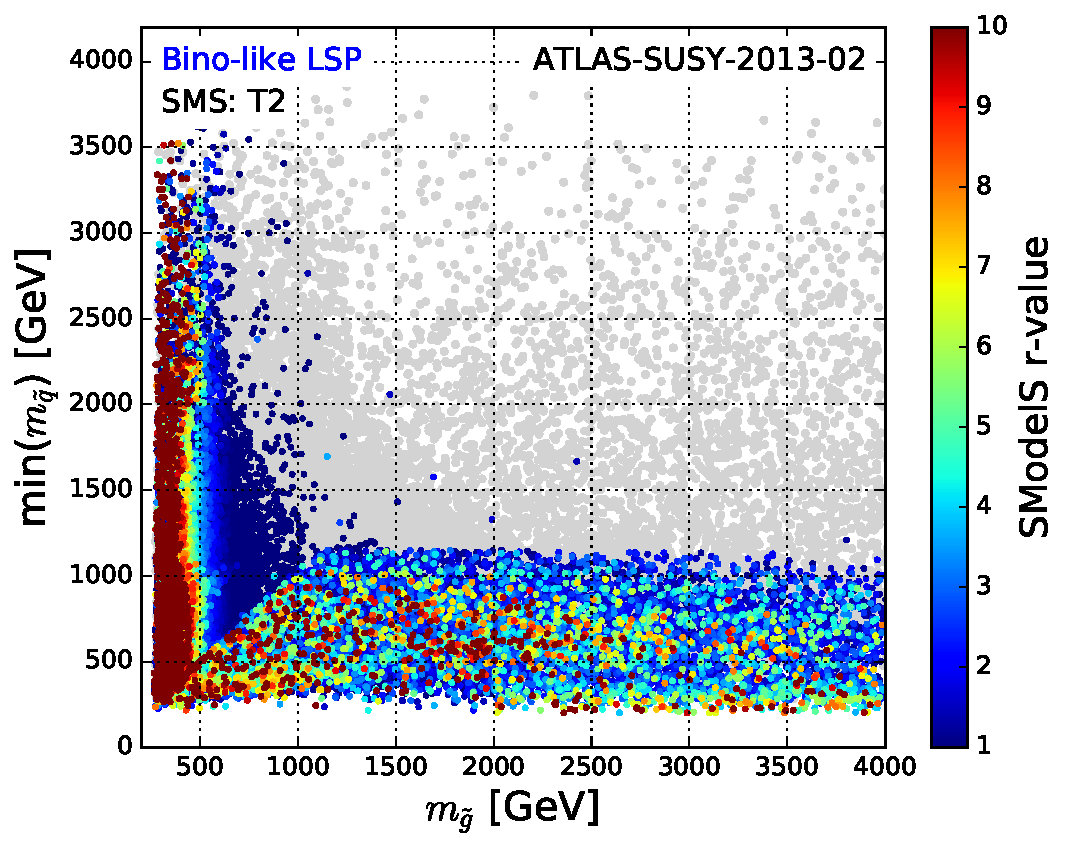
\includegraphics[width=0.49\textwidth]{PLOTS/Combination/ATLAS-SUSY-2013-02_Bino_SMS_T2_Glu_Squ.pdf}}
\subfigure
{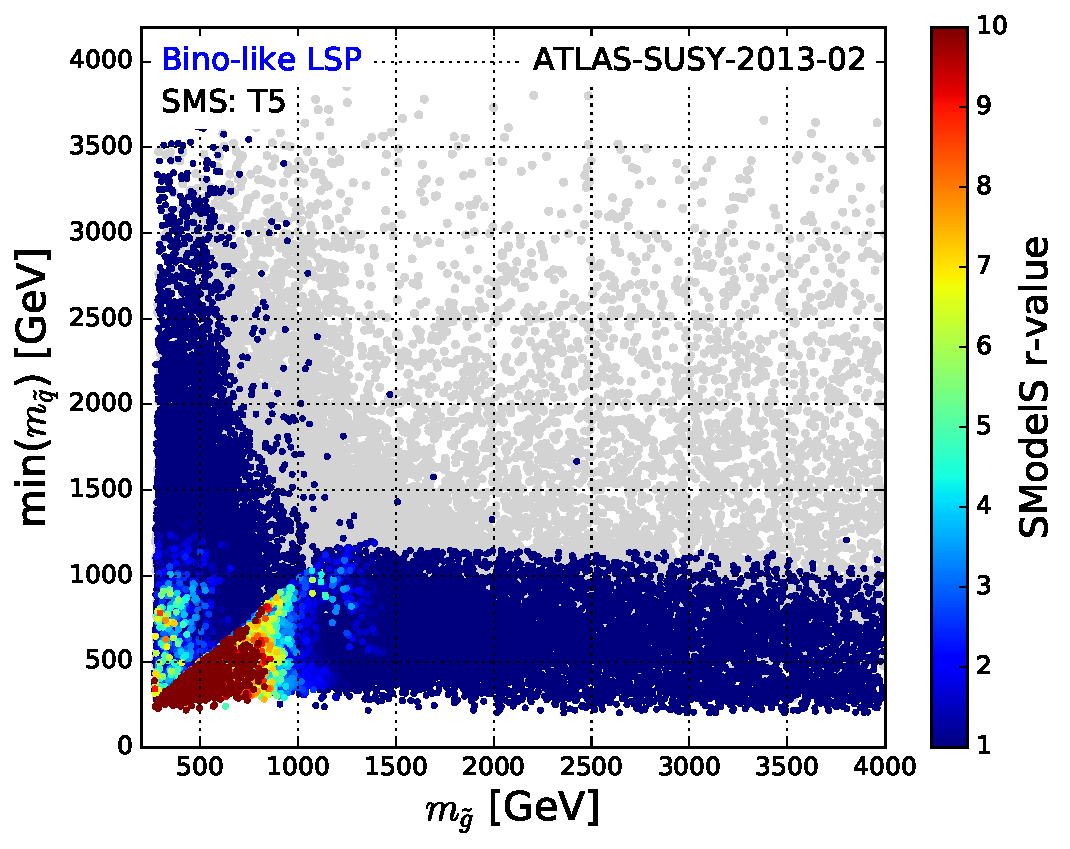
\includegraphics[width=0.49\textwidth]{PLOTS/Combination/ATLAS-SUSY-2013-02_Bino_SMS_T5_Glu_Squ.pdf}}
\subfigure
{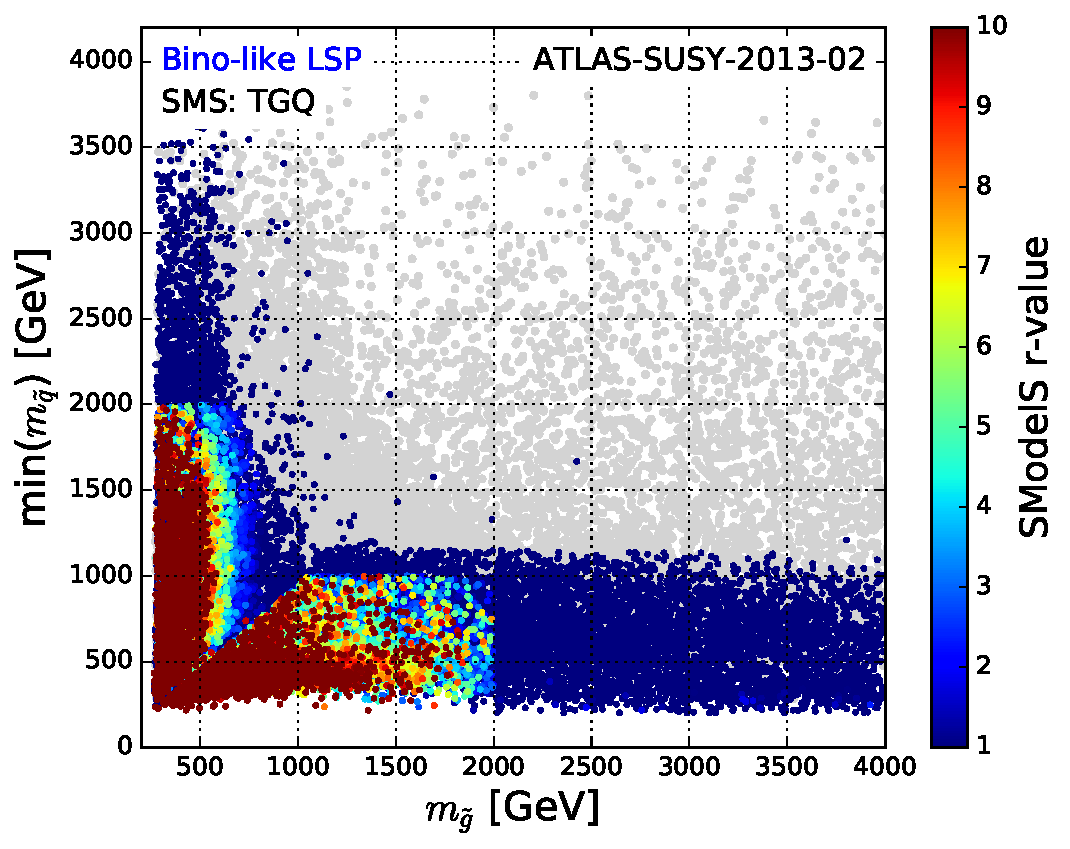
\includegraphics[width=0.49\textwidth]{PLOTS/Combination/ATLAS-SUSY-2013-02_Bino_SMS_TGQ_Glu_Squ.pdf}}
\subfigure
{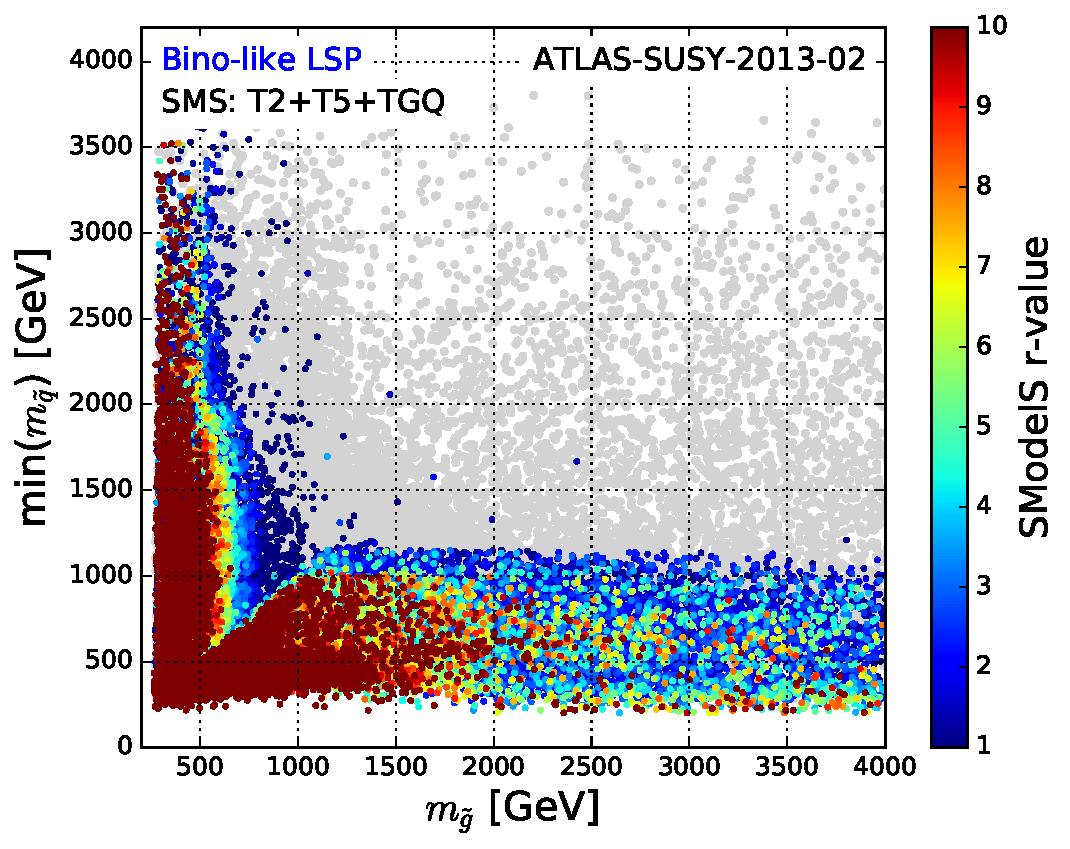
\includegraphics[width=0.49\textwidth]{PLOTS/Combination/ATLAS-SUSY-2013-02_Bino_SMS_T2+T5+TGQ_Glu_Squ.pdf}}
\end{center}
\caption{BLAH} 
\end{figure}

\begin{figure}[!]
\begin{center}
\subfigure
{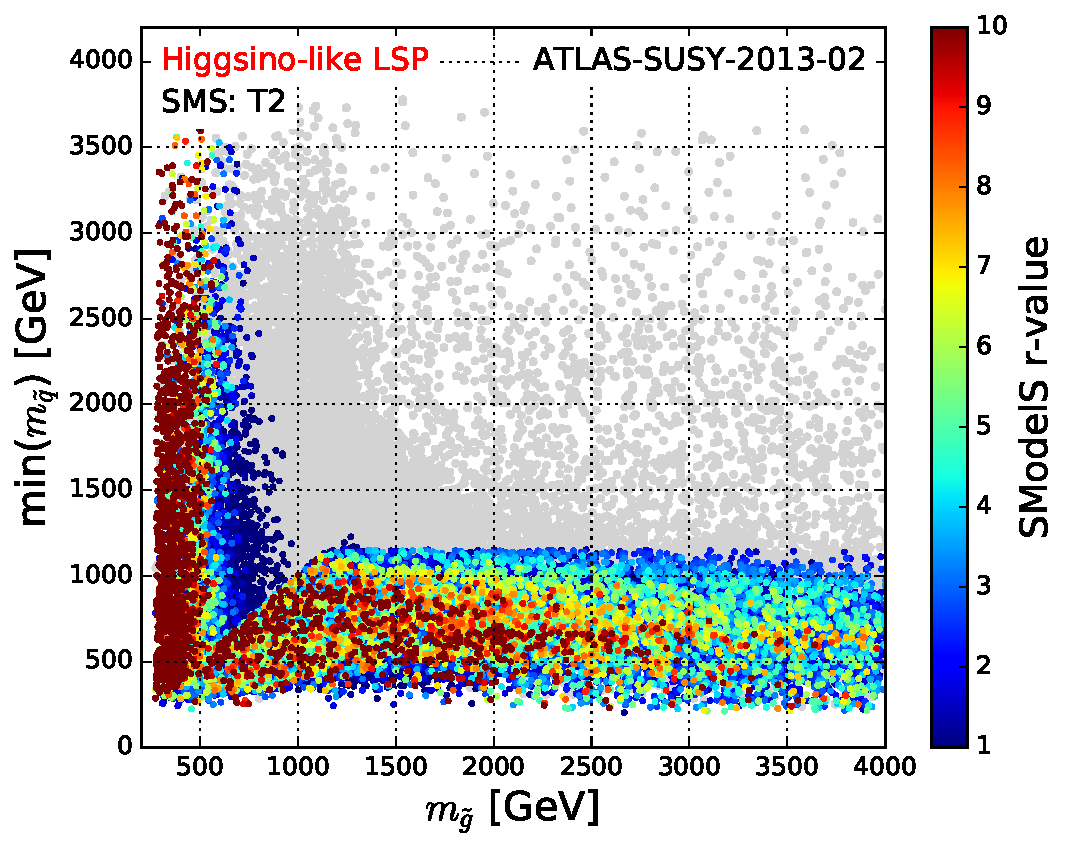
\includegraphics[width=0.49\textwidth]{PLOTS/Combination/ATLAS-SUSY-2013-02_Higgsino_SMS_T2_Glu_Squ.pdf}}
\subfigure
{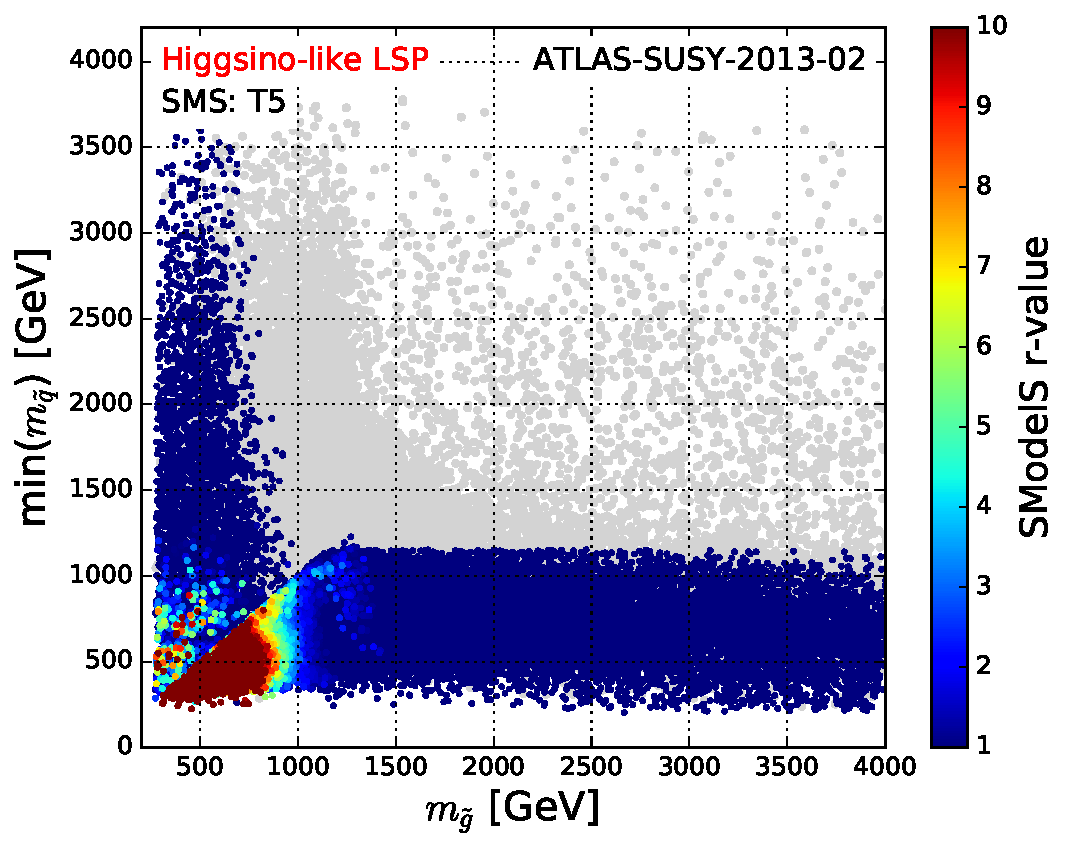
\includegraphics[width=0.49\textwidth]{PLOTS/Combination/ATLAS-SUSY-2013-02_Higgsino_SMS_T5_Glu_Squ.pdf}}
\subfigure
{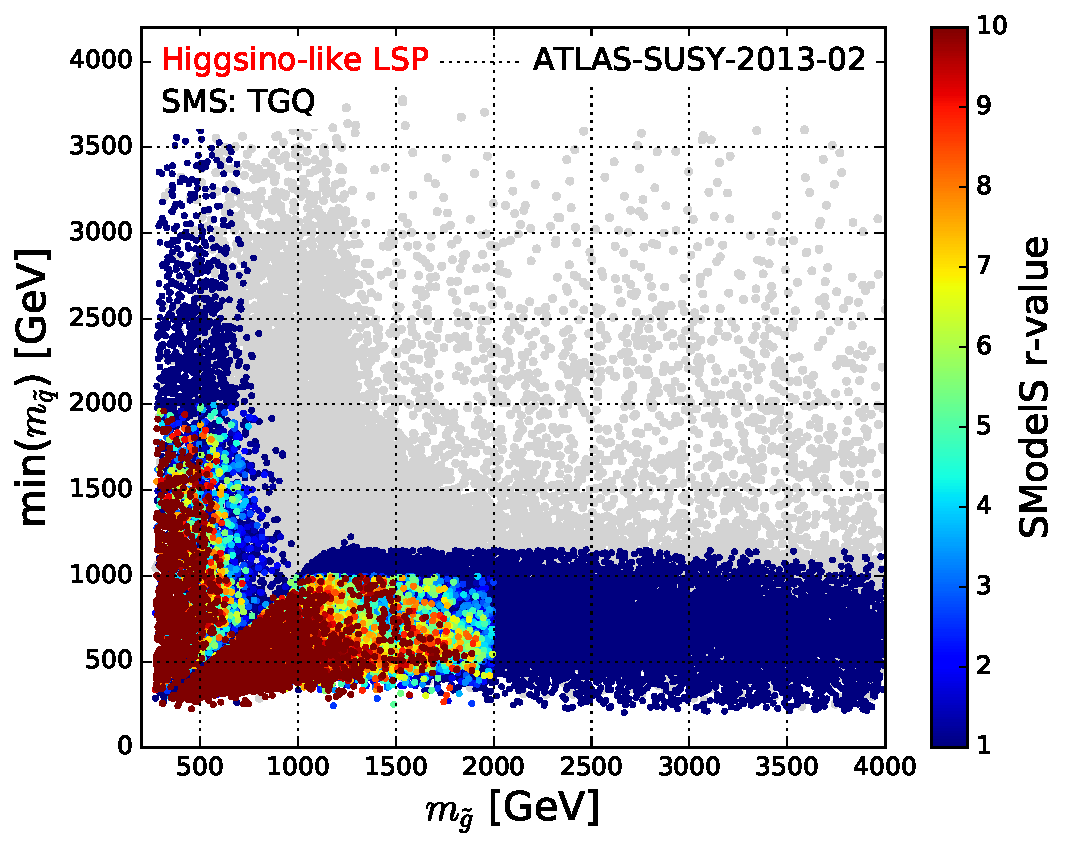
\includegraphics[width=0.49\textwidth]{PLOTS/Combination/ATLAS-SUSY-2013-02_Higgsino_SMS_TGQ_Glu_Squ.pdf}}
\subfigure
{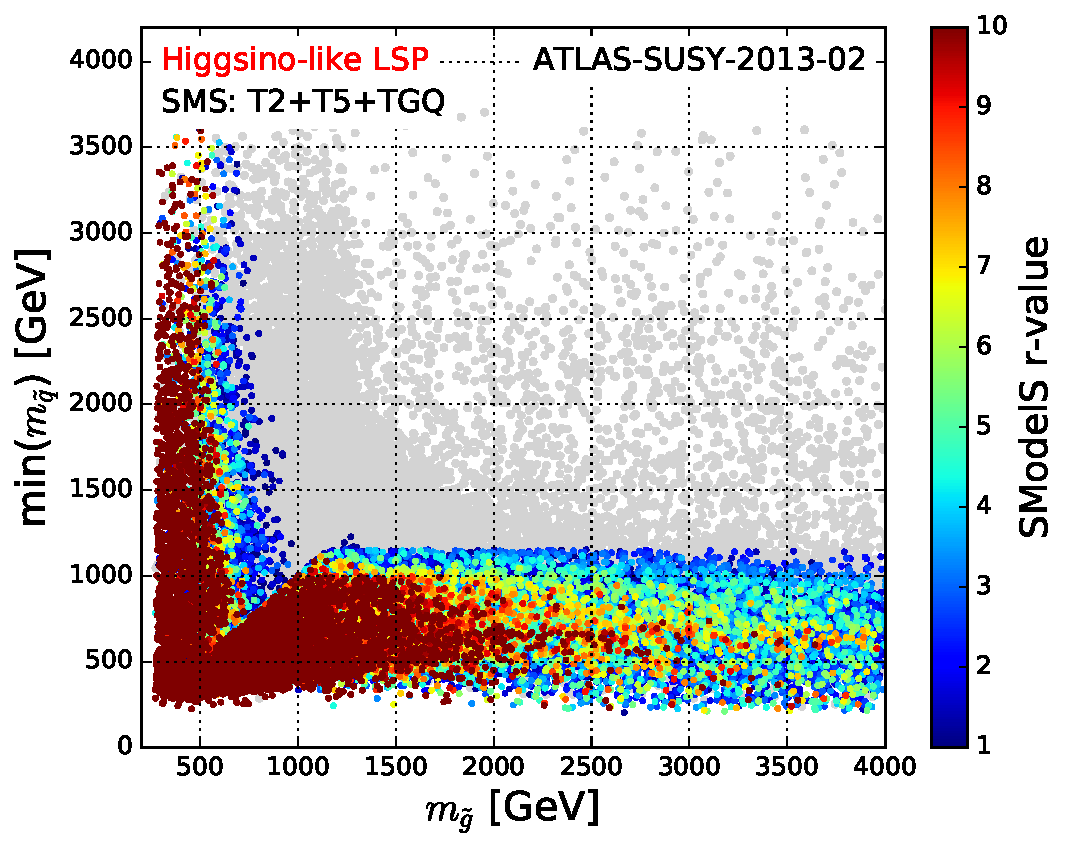
\includegraphics[width=0.49\textwidth]{PLOTS/Combination/ATLAS-SUSY-2013-02_Higgsino_SMS_T2+T5+TGQ_Glu_Squ.pdf}}
\end{center}
\caption{BLAH} 
\end{figure}



\bibliographystyle{JHEP}
\bibliography{references}


\end{document}
